\documentclass[12pt]{report}

%%%%%%%%%%%%%%%%%%%%%%%%%%%%%%%%%%%%%%%%%
% ESTILOS
\usepackage{xcolor}

% tablas
\usepackage{booktabs}  % Para líneas horizontales mejoradas
\usepackage{array}     % Para ajustar el espacio vertical en las celdas
\usepackage{rotating}  % Para rotar tablas
\usepackage{adjustbox} % Para ajustar texto a casillas
\usepackage{colortbl}  % PAra colorear celdas
\usepackage{longtable}


%%%%%%%%%%%%%%%%%%%%%%%%%%%%%%%%%%%%%%%%


% Paquetes LaTeX y estilos globales
\usepackage[utf8]{inputenc}
\usepackage{multicol}
\usepackage{xcolor}
\usepackage{subfigure}
\usepackage[spanish]{babel}
\usepackage[utf8]{inputenc}
\usepackage{graphicx}
\usepackage{titlesec}
\usepackage[bookmarks,breaklinks,colorlinks=true,allcolors=blue]{hyperref}
\usepackage{listings}
\usepackage{inconsolata}
\usepackage{float}
\usepackage{eso-pic}
\usepackage[framemethod=tikz]{mdframed}

\usepackage[square,numbers]{natbib}
\AtBeginDocument{
  \renewcommand{\bibsection}{\chapter{\bibname}}
} % Bibliografia en capitulo numerado

\usepackage{geometry}
\usepackage{amsmath}
\usepackage{parskip}
\usepackage[official]{eurosym}
\usepackage{todonotes}
\usepackage{csquotes}
% Formato del título de capítulos y secciones
\titleformat{\chapter}[block]{\titlerule[0.8pt]\normalfont\huge\bfseries}{\thechapter.}{.5em}{\Huge}[{\titlerule[0.8pt]}]
\titlespacing*{\chapter}{0pt}{-19pt}{25pt}
\titleformat{\section}[block]{\normalfont\Large\bfseries}{\thesection.}{.5em}{\Large}



% Formato del código fuente con lstlisting
\lstset{
  basicstyle=\ttfamily,
  breaklines=true,
}

% Márgenes
\geometry{
    a4paper,
    margin=2.75cm
}

% Limite de profundidad del índice
\setcounter{tocdepth}{2}

% Indentación de párrafos
\setlength{\parindent}{1cm}

\renewcommand{\lstlistingname}{Extracto de código}
\renewcommand*{\lstlistlistingname}{Índice de extractos de código}

\definecolor{US_red}{cmyk}{0, 1, 0.65, 0.34}
\definecolor{US_yellow}{cmyk}{0, 0.3, 0.94, 0}

\mdfdefinestyle{US_style}{backgroundcolor=US_yellow!20, font=\bfseries, hidealllines=true}

% Comienzo del documento
\begin{document}

    % Portada y secciones no numeradas
    \begin{center}
\vspace*{1cm}

%\includegraphics[width=0.25\textwidth]{fig/ilustracion.png}

\includegraphics[width=0.3\textwidth]{fig/logoUNC.png}
%{\color{US_red} \rule{\linewidth}{0.75mm} }

\vspace*{1cm}
\begin{large}
UNIVERSIDAD NACIONAL DE CÓRDOBA 

FACULTAD DE CIENCIAS EXACTAS FÍSICAS Y NATURALES
\end{large}


\vspace*{0.1in}
\AddToShipoutPictureBG*{\AtPageLowerLeft{%
  \color{US_red!20}\rule{.25\paperwidth}{\paperheight}}}


\textbf{\huge CASE MANAGEMENT SYSTEM}

{\Large \textbf{Sistema de Gestión de Casos Judiciales}}
        

\vspace*{.2in}

{\large Realizado por}\\
\textbf{\Large Julieta Abigail Prieto} % Aquí su nombre

\vspace*{1cm}
\begin{mdframed}[style=US_style]
\centering
\textbf{Proyecto Integrador de la Carrera}\\
{\large Ingeniería en Computación} 

\vspace*{0.2in}

\textbf{Dirigido por}\\
{\large Danilo Páez}\\
\vspace*{0.2in}
\textbf{Co-dirigido por}\\
{\large Laura Díaz}\\

\vspace*{0.2in}
\end{mdframed}


\vspace*{.6in}
\textbf{Córdoba, Argentina}\\
\textbf{Enero del 2024}
\vspace*{0.2in}
\end{center}


\thispagestyle{empty} % Impide que se incluya número de página en la portada
\clearpage\setcounter{page}{1} % Comienza a incluir números de página a partir de aquí
\pagenumbering{roman} % En números romanos
    
    % Índice del documento y de figuras
    \begingroup
        % Los enlaces son normalmente azules, pero en los índices se configuran a negro
        % para que no aparezca todo azul
        \hypersetup{linkcolor=black}
        \tableofcontents
        \listoffigures
        \lstlistoflistings
    \endgroup
    
    % Cambia el estilo de números de página a normal
    \clearpage\pagenumbering{arabic}
    
    % Capítulos del trabajo
    \chapter{Introducción}
\label{cap:introduccion}

\section{Introducción}
\label{sec:introduccion:intro}
En este capítulo se delimita el contexto de la tesis, al mismo tiempo que se describen los objetivos, el alcance y la estructura de este documento.

\section{Contexto del PI}
\label{sec:introduccion:contexto}
El origen de este producto surgió a raíz del contacto con el laboratorio IALAB, quienes solicitaron el desarrollo de un sistema de gestión diseñado específicamente para potenciar y optimizar el Patrocinio Jurídico de la Facultad de Derecho de la Universidad de Buenos Aires.

El ``Patrocinio Jurídico Gratuito'', con casi un siglo de dedicación, se erige como un proyecto comprometido con la provisión de asistencia legal a aquellos en situación de vulnerabilidad económica y social. Esta iniciativa, integrada como práctica profesional en el plan de estudios de la carrera de abogacía, se distingue como un servicio singular en el país.

La problemática identificada en la administración de casos por parte de esta entidad se centra en la utilización actual de herramientas como TRELLO, un software de pago empleado para la gestión de casos, y Google Forms como sistema de recopilación de datos. Sin embargo, estas soluciones no satisfacen completamente las necesidades específicas del organismo, que requiere un software integral para la gestión, organización y automatización parcial de sus procesos.

En esta fase del proyecto, se busca reemplazar y unificar el sistema de gestión de casos, como así también automatizar eficientemente la carga de formularios en el sistema, contribuyendo un producto de valor al Proyecto Patrocinio.

El desarrollo de este sistema representa la concepción de una primera base que servirá como cimiento para futuras expansiones. Este enfoque busca establecer una plataforma modular y versátil que aborde las necesidades actuales del patrocinio jurídico de la UBA.



\section {Objetivo General del Proyecto}
\label{sec:objetivos:generales}
Diseñar e implementar un software integral de gestión de casos para el patrocinio jurídico de la Universidad de Buenos Aires (UBA).

\section {Objetivos Específicos del Proyecto}
\label{sec:objetivos:especificos}

\begin {enumerate}
\item Analizar y comprender las limitaciones del software actualmente utilizado, TRELLO, y del sistema de recolección de datos mediante Google Forms.
\item Relevar, analizar y construir los requisitos tanto funcionales como no-funcionales solicitados por el cliente.
\item Diseñar e implementar una arquitectura modular que permita una gestión eficiente y escalable de casos.
\item Diseñar una estructura de base de datos que permita una gestión eficaz de la información.
\end{enumerate}

\section {Alcance del Proyecto}
\label{sec:alcance}
En el marco de este proyecto, se abordarán los siguientes procesos:

\begin {enumerate}
\item Diseño, Desarrollo e Implementación del Software de Gestión de Casos:

El enfoque principal estará en la concepción, desarrollo y despliegue de un software de gestión de casos diseñado específicamente para satisfacer las necesidades del patrocinio jurídico de la Universidad de Buenos Aires (UBA).

\item Integración con Google Forms:

Se incorporará la integración de Google Forms para automatizar la carga eficiente de formularios en el sistema, mejorando así la recopilación de datos y simplificando el proceso para el patrocinio jurídico.

\item Optimización del Sistema de Solicitud y Control Histórico:

El software se orientará hacia la facilitación y optimización del sistema de solicitud, asegurando un control histórico efectivo de los casos por comisión. Esto se traducirá en una gestión más eficiente de los procesos asociados con la presentación y seguimiento de casos.

\item Registro Histórico por Comisión:

Se contemplará la mejora del registro histórico mediante la posibilidad de cargar archivos relevantes y comentarios asociados a cada caso. Esto permitirá un seguimiento más detallado y completo de la evolución de los casos a lo largo del tiempo.
\end{enumerate}

\section{Acrónimos y Abreviaturas}
\label{sec:acronimos}

En el presente documento, se utilizan los siguientes acrónimos y abreviaturas:

\begin{table}[H]
    \centering
    \begin{tabular}{|c|p{10cm}|}
    \hline
         \textbf{Acrónimos} & \textbf{Descripción}\\
    \hline
         API & Interfaz de Programación de Aplicaciones (por sus siglas en inglés, \textit{Application Programming Interface})\\
    \hline
         HTTP & Protocolo de Transferencia de Hipertexto (por sus siglas en inglés, \textit{Hypertext Transfer Protocol})\\
    \hline
         IP & Protocolo de Internet (\textit{Internet Protocol})\\
    \hline
         JSON & Notación de Objetos de JavaScript (\textit{JavaScript Object Notation}) \\
    \hline
         REST & Transferencia de Estado Representacional (\textit{Representational State Transfer}) \\
    \hline
        DNS & Sistema de Nombres de Dominio (\textit{Domain Name System}) \\
    \hline
        SSL/TLS & Capa de Conexión Segura / Protocolo de Seguridad de la Capa de Transporte (\textit{Secure Sockets Layer / Transport Layer Security}) \\
    \hline
        SQL & Lenguaje de Consulta Estructurada (\textit{Structured Query Language}) \\
    \hline
        CORS & Intercambio de recursos de origen cruzado (\textit{Cross Origin Resource Sharing})\\
    \hline
         CSRF & Falsificación de Petición en Sitios Cruzados (\textit{Cross-Site Request Forgery}) \\
    \hline
         NIST & Instituto Nacional de Estándares y Tecnología (\textit{National Institute of Standards and Technology}) \\
    \hline
        CI & Integración Continua (\textit{Continuous Integration}) \\
    \hline
        CD & Entrega Continua (\textit{Continuous Delivery}) \\
    \hline
        UBA & Universidad de Buenos Aires \\
    \hline
        UNC & Universidad Nacional de Córdoba \\
    \hline
       ASGI & Interfaz de Puerta de Enlace Asíncrona del Servidor (\textit{Asynchronous Server Gateway Interface}) \\
    \hline
        WSGI & Interfaz de Puerta de Enlace del Servidor Web (\textit{Web Server Gateway Interface}) \\
    \hline
        
    \end{tabular}
    \caption{Lista de Acrónimos y Abreviaturas}
    \label{tab:my_label}
\end{table}

    \chapter{Requerimientos y Especificaciones}\label{cap:disenio}

\section{Introducción}
En este capítulo se detalla en su totalidad el producto de la plataforma de gestión y automatización para el proceso de selección de los casos del Patrocinio Jurídico Gratuito de la UBA. En este se describen sus funcionalidades, especificaciones y limitaciones en cuanto a su utilización.

\section{Alcance del Producto}
Este producto está orientado a profesores y tomadores de casos del Patrocinio Jurídico Gratuito, con el fin de facilitar y mejorar la eficiencia del sistema de solicitud y control histórico de los casos, asegurando una experiencia intuitiva en su utilización.

El alcance de esta plataforma abarca el proceso desde la recepción de datos a través de Google Forms, la integración de la información en el sistema, la gestión de los casos en la asignación a comisiones y, finalmente, el seguimiento y gestión de los casos por parte de los profesores de la comisión. 

\section{Referencias}
A continuación, se presenta una lista detallada de las tecnologías utilizadas en el desarrollo del proyecto, acompañadas de enlaces a sus respectivas documentaciones. Estos recursos fueron seleccionados estratégicamente para facilitar el desarrollo, la implementación y el mantenimiento del sistema.


\begin{table}[H]
    \centering
    \begin{tabular}{|p{11cm}|p{4cm}|}
        \hline
        \textbf{Recurso} & \textbf{Sitio Web} \\
        \hline
        Documentación de Python 3. & \href{https://docs.python.org/3/}{Python3} \\
        \hline
        Documentación de Django 4.1. & \href{https://docs.djangoproject.com/en/4.1/}{Django} \\
        \hline
        Documentación de Django Rest Framework, una extensión de Django para construir APIs. & \href{https://www.django-rest-framework.org/#quickstart}{Django-Rest} \\
        \hline
        Documentación de PostgreSQL para la base de datos. & \href{https://www.postgresql.org/docs/current/}{PostgreSQL} \\
        \hline
        Documentación Django-docutils para la automatización de la documentación de la API. & \href{https://docs.djangoproject.com/en/4.1/ref/contrib/admin/admindocs/}{Django-docutils} \\
        \hline
        Documentación del lenguaje Gherkin para listar los requerimientos. & \href{https://docs.behat.org/en/v2.5/guides/1.gherkin.html}{Gherkin} \\
        \hline
        Documentación de Nginx para un servidor web y/o proxy inverso. & \href{http://nginx.org/en/docs/}{Nginx} \\
        \hline
        Documentación de Gunicorn, un servidor HTTP Python WSGI para UNIX. &
        \href{https://gunicorn.org/#docs}{Gunicorn} \\
        \hline
        Documentación de React, una biblioteca de JavaScript para construir interfaces Reactivas de usuario. & \href{https://es.react.dev/reference/react}{React}\\
        \hline
        Documentación de Material-UI, una biblioteca de componentes de interfaz de usuario para React. & \href{https://mui.com/material-ui/getting-started/}{MUI} \\
        \hline
        Documentación de Beautiful Drag and Drop para implementar funcionalidades de arrastrar y soltar. & \href{https://github.com/atlassian/react-beautiful-dnd}{React-Beautiful-DND} \\
        \hline
        Documentación de Django Channels para el manejo de conexiones en tiempo real a Django. & \href{https://channels.readthedocs.io/en/latest/}{Channels} \\
        \hline
        Documentación de Daphne, un servidor ASGI (Asynchronous Server Gateway Interface) para aplicaciones asincrónicas con Django. & \href{https://docs.djangoproject.com/en/5.0/howto/deployment/asgi/daphne/}{Daphne}\\
        \hline
        Documentación de Docker. & \href{https://docs.docker.com/engine/}{Docker} \\
        \hline
        Documentación de Docker Swarm para la orquestación de contenedores. & \href{https://docs.docker.com/engine/swarm/}{Docker-Swarm}\\
        \hline
        Documentación de Robot Framework para la automatización de test. & \href{https://robotframework.org/robotframework/latest/RobotFrameworkUserGuide.html}{Robot-Framework}\\
        \hline
        Documentación de Selenium para la automatización de tareas desde el browser. & \href{https://robotframework.org/SeleniumLibrary/SeleniumLibrary.html}{Selenium}\\
        \hline
    \end{tabular}
    \caption{Recursos y Enlaces de Documentación}
    \label{tab:recursos_documentacion}
\end{table}



\newpage

\section{Descripción General}

\subsection{Perspectiva del Producto}
El producto surge para abordar una necesidad administrativa identificada en la organización del Patrocinio Jurídico de la UBA. Actualmente, los formularios de los solicitantes se envían automáticamente por Google Forms mediante correo electrónico y luego se cargan manualmente en un software pago, Trello. Esta metodología presenta desafíos de integración y no se ajusta completamente a los requisitos específicos de la organización. La solución propuesta busca mejorar la organización y gestión de casos mediante un software que se integre de manera eficiente con Google Forms.

El sistema se integrará sin inconvenientes con Google Forms para facilitar la captura de datos relacionados con casos judiciales y nuevos clientes. Este enfoque optimizará el proceso de solicitud, selección y gestión de casos, brindando a los usuarios finales una experiencia más sencilla y ágil. La interfaz de usuario, diseñada intuitiva y amigablemente, seguirá las mejores prácticas de diseño centrado en el usuario, asegurando eficiencia y transparencia en la experiencia del usuario.

\subsection{Funciones del Producto}
El sistema desarrollado proporciona un conjunto integral de funciones diseñadas para satisfacer las necesidades específicas de la gestión de casos judiciales y su asignación a las comisiones. Integra de manera fluida con Google Forms, permitiendo la captura eficiente de datos relacionados con casos judiciales y nuevos clientes. Facilita la selección y asignación de casos a comisiones. La interfaz de usuario intuitiva permite el seguimiento detallado de cada caso a lo largo de su ciclo de vida, facilitando una gestión efectiva y transparente por parte de los profesores de las comisiones. Incluye un sistema de notificaciones vía email y alertas para anunciar ciertos eventos. La interfaz de usuario, es intuitiva, fácil de navegar y brinda una experiencia eficiente, contribuyendo a mejorar la eficiencia, la transparencia y la efectividad en la gestión de casos y la selección de comisiones.

\subsection{Tipos de Usuarios y Características}
El sistema contempla varios tipos de usuarios, cada uno con funciones y características específicas para satisfacer sus necesidades dentro del proceso. Los roles principales incluyen:

\textbf{Administradores del Sistema}: Tienen acceso completo al sistema y la capacidad de gestionar usuarios y acceder a todas las funcionalidades. Su función principal es garantizar el correcto funcionamiento y la configuración adecuada del sistema.

\textbf{Profesores de Comisión}: Estos usuarios son responsables de revisar, evaluar y gestionar los casos asignados a su comisión. Pueden acceder a la información detallada de cada caso, realizar comentarios, asignar tareas y seguir el progreso de manera integral.

\textbf{Solicitantes}: Son los usuarios encargados de presentar casos judiciales mediante Google Forms. Aunque no tienen acceso directo a la plataforma, desempeñan un papel crucial al ingresar casos y nuevos clientes a través de Google Forms, contribuyendo así al flujo eficiente de datos en el sistema.

\textbf{Administradores de Casos}: Más conocidos como \textbf{Tomadores de Caso}, este rol se ocupa de la gestión específica de los casos, desde su recepción hasta su asignación a una comisión. Pueden revisar la información proporcionada por los solicitantes y asignar casos a las comisiones correspondientes.




\subsection{Entorno Operativo}

La plataforma estará diseñada para operar en un entorno que cumpla con los siguientes requisitos:

\subsubsection{Requisitos de Servidor}
La aplicación está diseñada para ser accesible desde cualquier dispositivo con capacidad para ejecutar contenedores Docker, lo que incluye sistemas operativos como Linux, Windows y macOS.

Se recomienda empezar al menos con:
\begin{itemize}
    \item 100 GB de almacenamiento libre
    \item 6 GB de RAM
    \item 2 núcleo de CPU
\end{itemize}

Estos requisitos proporcionarán una base para el despliegue inicial de la aplicación, asegurando un funcionamiento estable y eficaz. Se debe tener en cuenta que estos son requisitos mínimos y se puede considerar la posibilidad de aumentar estos recursos en función de la carga de trabajo y el crecimiento futuro de la aplicación.

\subsubsection{Navegadores Soportados}

\begin{itemize}
    \item Google Chrome. Se probó en la versión Versión 120.0.6099.130.
    \item Mozilla Firefox. Se probó en la versión 121.0.
\end{itemize}

\subsubsection{Conectividad}
Se requiere una conexión a Internet estable para el correcto funcionamiento de la integración con Google Forms y el acceso a la plataforma. La velocidad de la conexión afectará directamente la eficiencia en la carga y manejo de datos.

\subsubsection{Dispositivos Compatibles}
La plataforma está diseñada para ser accesible desde dispositivos con pantallas de tamaño mediano a grande, como computadoras de escritorio, laptops y tabletas. El acceso desde dispositivos móviles puede ser posible, pero la experiencia de usuario puede variar según el tamaño de la pantalla.




\section{Restricciones de Diseño e Implementación}
\begin{itemize}
    \item \textbf{Limitaciones a nivel de Interfaz}:  Se busca una interfaz gráfica simple e intuitiva que sea      semejante a la interfaz de Trello la cual, los usuarios finales están familiarizados. Para así facilitar la utilización para usuarios con pocos conocimientos en el ámbito de la informática.
    \item \textbf{Limitaciones presupuestarias}: Debido a que el organismo solicitante del producto no tiene presupuesto para la creación y mantenimiento del sistema. Este debe tener un costo bajo o nulo.
    \item \textbf{Seguridad y Privacidad}
    La plataforma debe seguir las mejores prácticas de seguridad para proteger la información confidencial de los casos judiciales y los datos de los usuarios. Se deben implementar mecanismos de autenticación y autorización, y se debe garantizar el cifrado de la comunicación entre el cliente y el servidor.
\end{itemize}


\section{Modelo Conceptual de Datos - DER}

En la construcción del Modelo Conceptual de Datos, se tomó la decisión de utilizar PostgreSQL como motor de búsqueda para la base de datos, basándonos en su destacada capacidad para respaldar las propiedades fundamentales del modelo ACID (Atomicidad, Consistencia, Aislamiento y Durabilidad). Estas características son esenciales para garantizar la integridad y confiabilidad de las transacciones en la base de datos.

Posteriormente, al interpretar la matriz de relaciones, se simplificó la visualización al omitir algunas tablas intermedias, para facilitar la comprensión del esquema general de la base de datos de manera más accesible.

Los diagramas subsiguientes se derivan de un modelo de base de datos que ha sido procesado y refinado hasta alcanzar la tercera forma normal, una práctica común con el propósito de optimizar la organización y estructura de los datos, evitando redundancias y asegurando consistencia.

Adicionalmente, como estrategia para simplificar el diseño y reducir la complejidad asociada al manejo de grandes volúmenes de datos, se ha decidido tratar las calles como cadenas de texto independientes de las localidades. Esta decisión se basa en la idea de no vincularlas geográficamente, evitando así la carga adicional que implicaría gestionar todas las calles de Argentina, la cual podría resultar significativa en términos de volumen de datos y complejidad operativa.

Consulte en el anexo, los Diagramas~\ref{mat:der}, \ref{mat:der2} y \ref{mat:der3} para visualizar las matrices de relaciones de entidades.



A continuación se presenta el diagrama de Entidad-Relación. En celeste se resalta la relación muchos a muchos, la cual ha sido reemplazada por una tabla intermedia denominada "board-user". Y en un azul mas oscura se representa la herencia de Person con User y Client.

\begin{figure}[H]
    \centering
    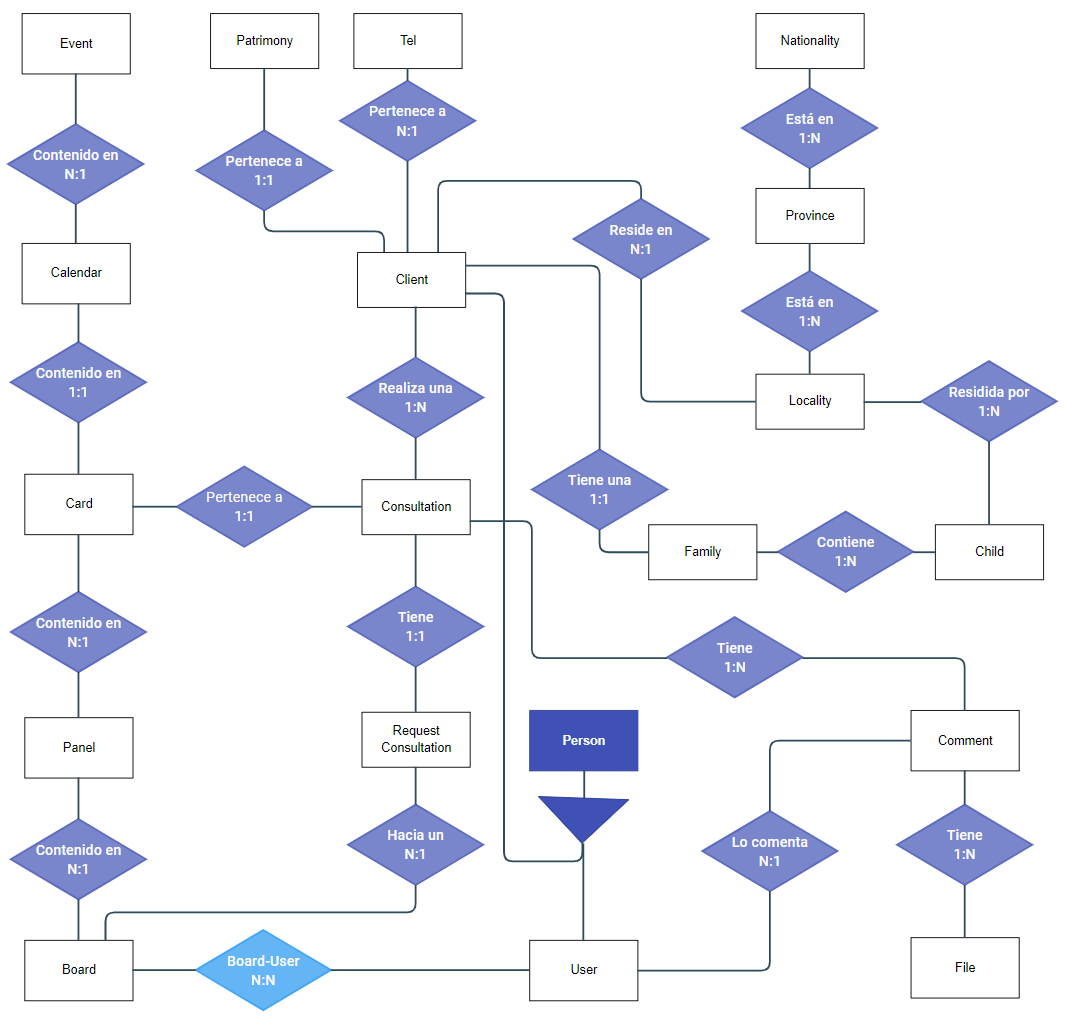
\includegraphics[width=1\linewidth]{fig/der.png}
    \caption{Diagrama Entidad Relación}
    \label{fig:der}
\end{figure}

\newpage

La implementación del modelo se lleva a cabo en Django. Sin embargo, para simplificar la explicación, se han omitido otras entidades relacionadas al usuario propias de Django, como tokens, grupos, etc. A continuación, se presenta el resultado visualizado mediante DBeaver, utilizado como gestor de la base de datos.

\begin{figure}[H]
    \centering
    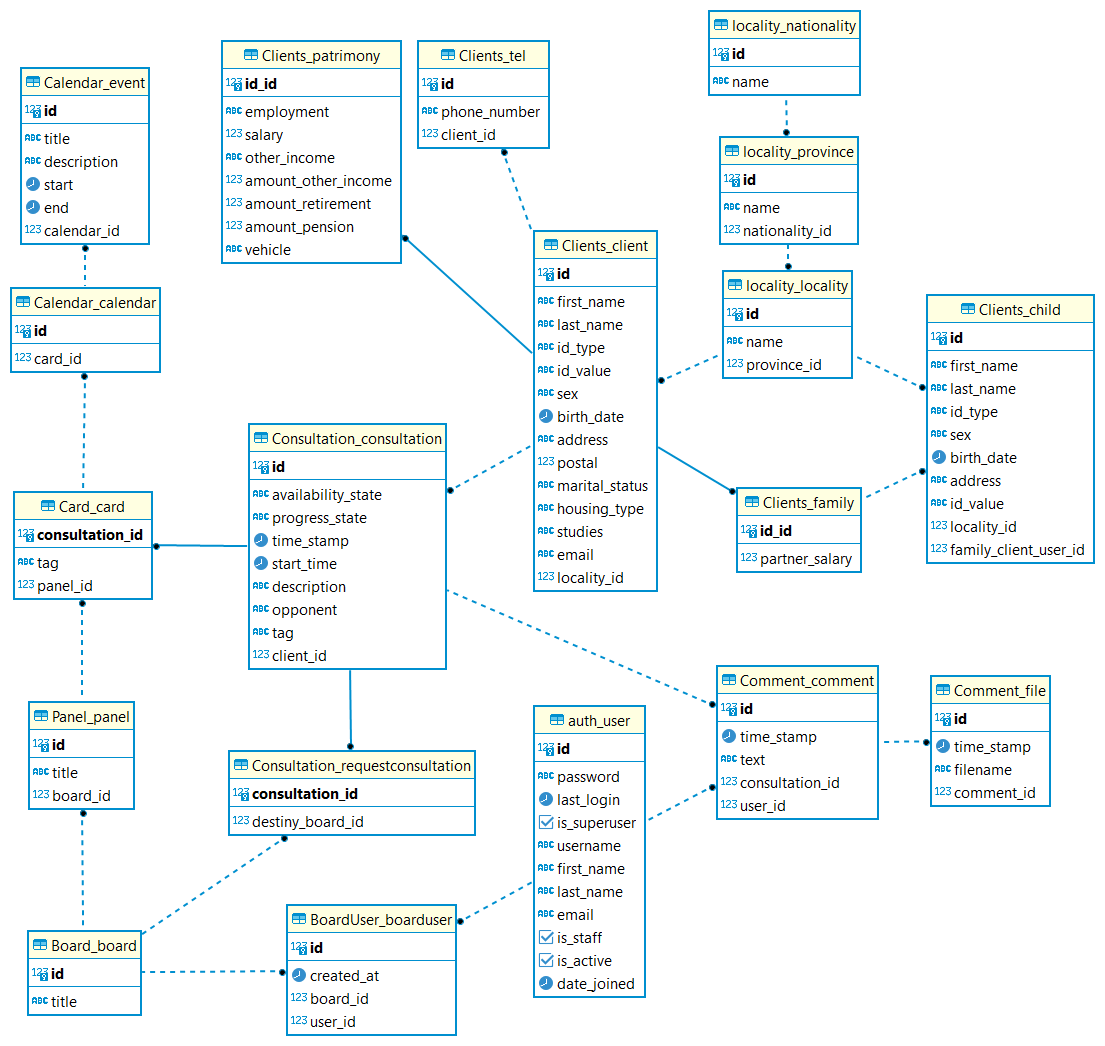
\includegraphics[width=1\linewidth]{fig/dbeaver.png}
    \caption{Implementación del Modelo Entidad Relación}
    \label{fig:dbeaver}
\end{figure}




\section{Requerimientos de Interfaces Externas}


En esta sección, se presenta los requerimientos de de Interfaces, que sirve como un elemento para la visualización y estructuración de la interfaz de usuario. A continuación, se exhiben los mockup representativos del diseño propuesto para la interfaz gráfica de usuario (GUI).

\subsection{Consultoría}

La Figura \ref{fig:gui-consultancy} exhibe un mockup que encapsula la apariencia y disposición previstas de la interfaz de usuario, específicamente en el contexto de la funcionalidad de consultoría.

Dada la necesidad de lograr una experiencia intuitiva, se estableció como requisito la implementación de tableros para la asignación de casos, tomando como referencia la utilización previa de Trello en el organismo.

\begin{figure}[h]
\centering
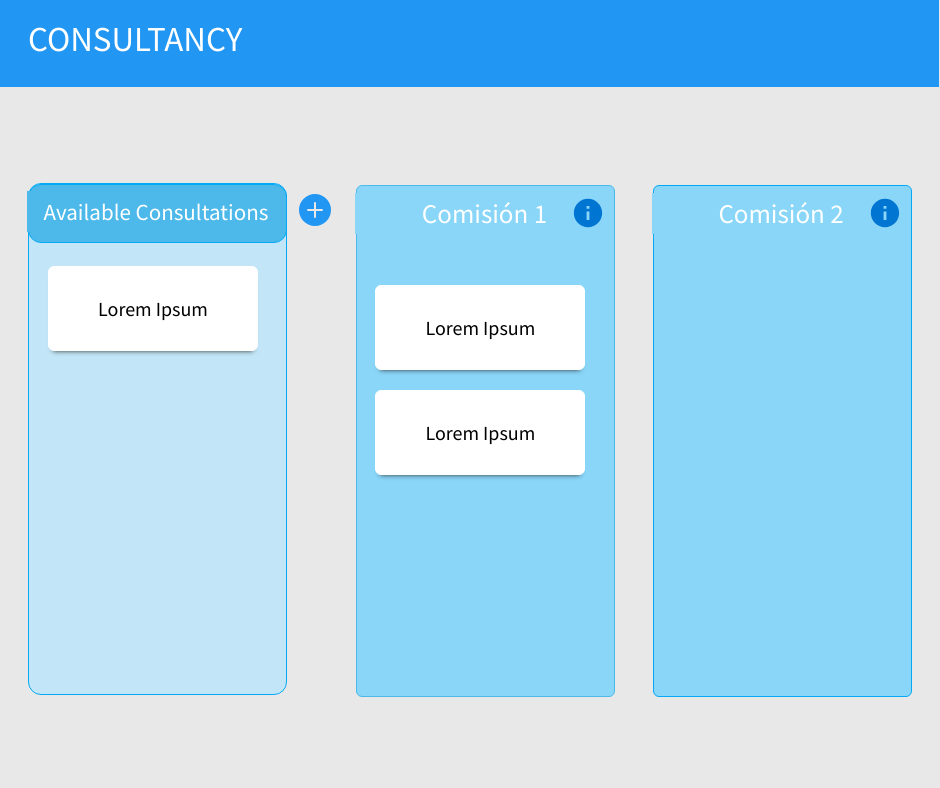
\includegraphics[width=1\linewidth]{fig/GUI-consultancy.png}
\caption{Mockup de la Interfaz Gráfica de Usuario (GUI) para la Página Consultoría}
\label{fig:gui-consultancy}
\end{figure}


A la izquierda, se ubica el tablero de casos sin asignar, mientras que a la derecha se presentan los tableros destinados para enviar las solicitudes de asignación del caso a las diversas comisiones. Cada tarjeta (card) en estos tableros representa una consulta específica.

Adicionalmente, se incorporan dos elementos clave para la interacción:
\begin{itemize}
    \item El botón ``+''  facilita la creación de nuevas consultas.
    \item El botón de información proporciona detalles específicos sobre la comisión correspondiente.
\end{itemize}



\subsection{Tablero de Trabajo para Cada Comisión}

El diseño del tablero de trabajo adopta una lógica similar a la implementada en la funcionalidad de consultoría, manteniendo paneles organizativos que permiten la manipulación intuitiva de tarjetas mediante el sistema de arrastre y soltar.


\begin{figure}[H]
\centering
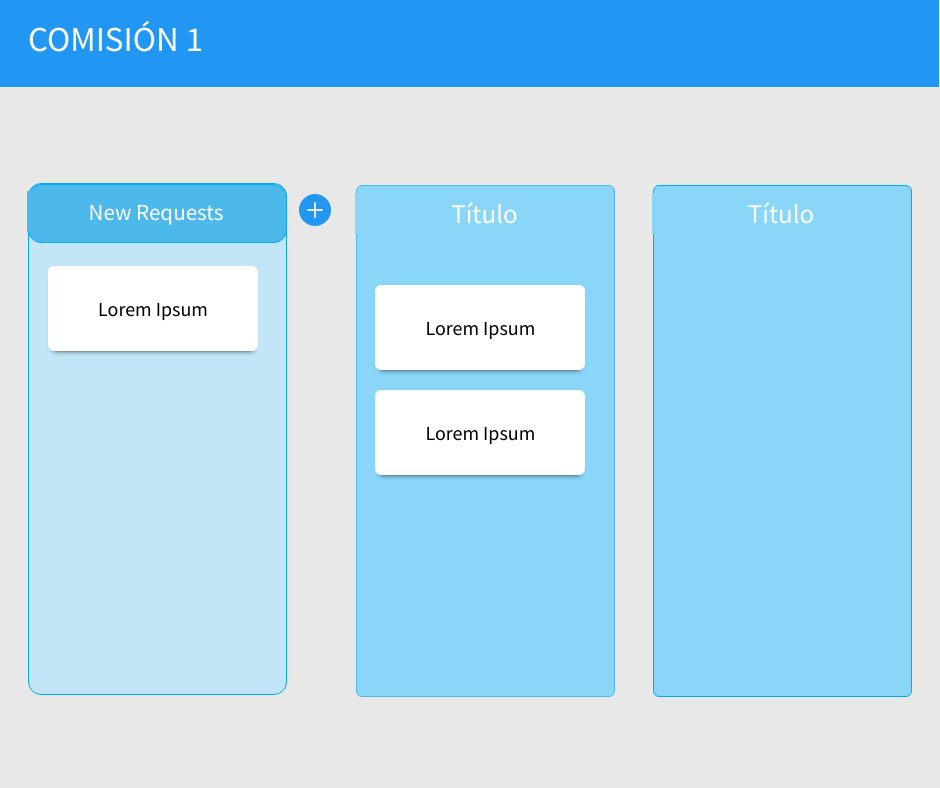
\includegraphics[width=1\linewidth]{fig/board.png}
\caption{Mockup de la Interfaz Gráfica de Usuario (GUI) para el Tablero de Comisión}
\label{fig:board}
\end{figure}


En el lado izquierdo de la imagen, se sitúa el panel de entrada, destinado a recibir las solicitudes entrantes. A la derecha, se encuentran paneles específicos de la comisión, ajustados según las necesidades particulares. La funcionalidad del botón "+" simplifica la creación de paneles adicionales. Por ejemplo, se podrían generar tableros para representar el estado de la consulta o agruparlos según profesor.

Finalmente, las tarjetas blancas dentro de los paneles representan cada consulta con una etiqueta referente.


\subsection{Inicio de Sesión}
Para garantizar la seguridad y autenticación de los usuarios, se ha implementado se tiene como requisito una interfaz de inicio de sesión al sistema. La Figura \ref{fig:enter-label} presenta el diseño visual asociado con la página de inicio de sesión.

\begin{figure}[H]
    \centering
    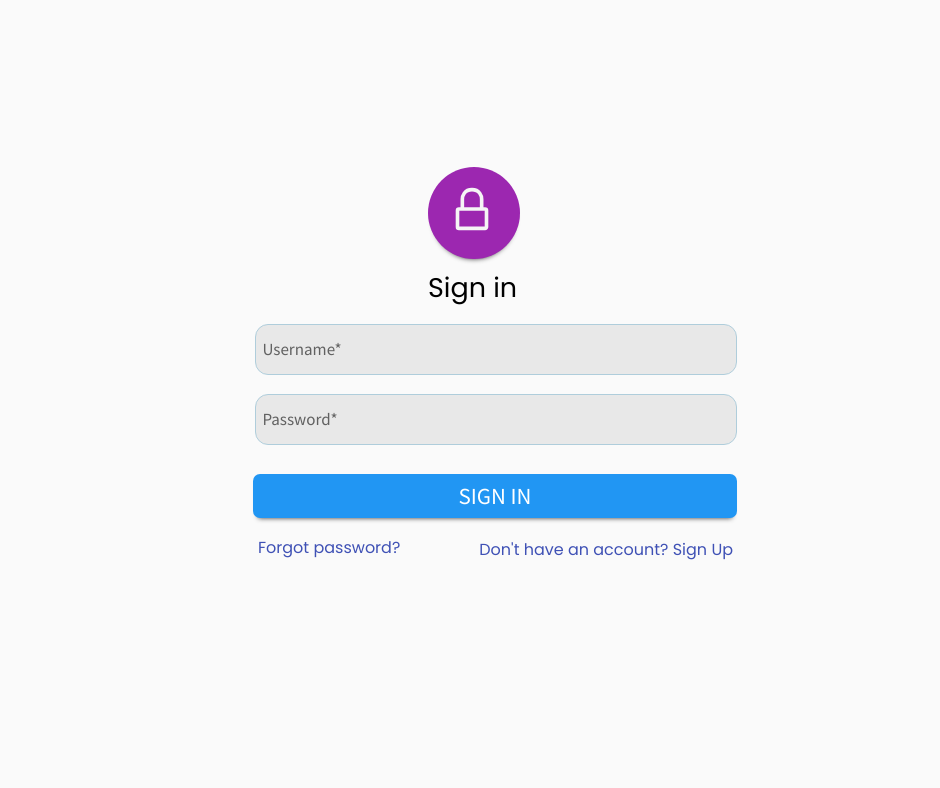
\includegraphics[width=1\linewidth]{fig/signin.png}
    \caption{Mockup de la Interfaz de Inicio de Sesión}
    \label{fig:signin}
\end{figure}

Como se evidencia en esta interfáz, el requisito de inicio de sesión solicita la introducción de un usuario y contraseña para acceder al sistema. Además, se ha incorporado la opción de recuperar la contraseña en caso de olvido, así como la capacidad de crear una nueva sesión para los usuarios que aún no cuentan con una cuenta registrada.


\subsection{Información de la Consulta}

Un requisito fundamental del sistema es la capacidad de visualizar la información detallada de cada consulta. Esta sección abarca diversos aspectos esenciales, incluyendo datos específicos de la consulta, una sección dedicada a comentarios, y una interfaz de calendario para gestionar fechas clave.

La Figura \ref{fig:info-consult-gui} presenta un mockup que ilustra la propuesta visual para la interfaz de información de consulta.

\begin{figure}[H]
\centering
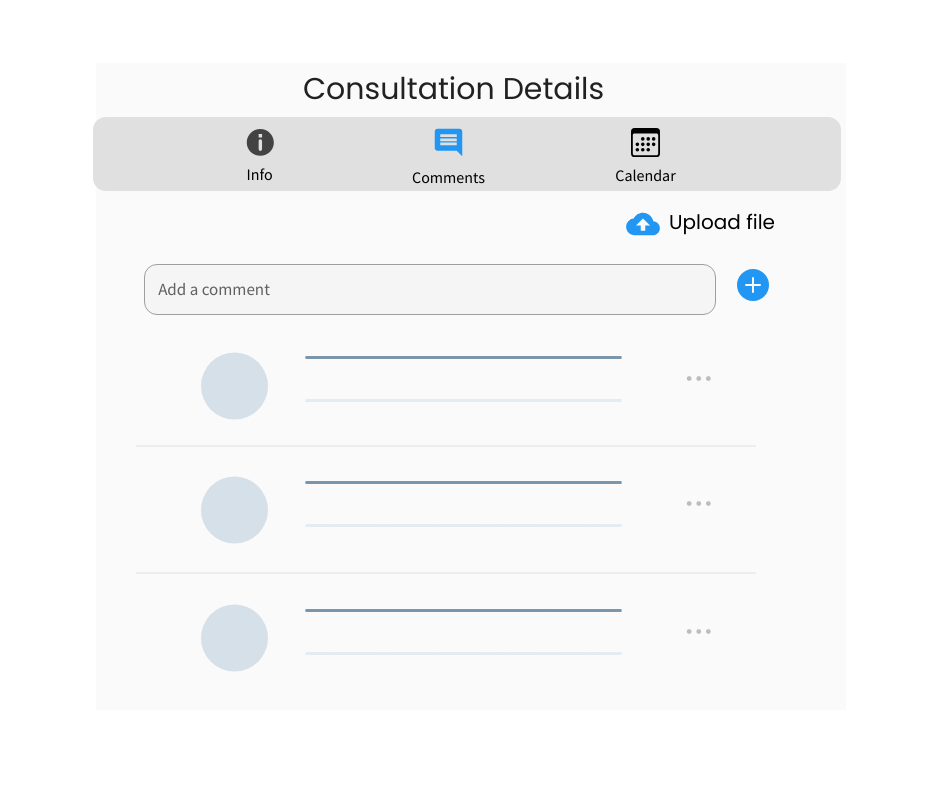
\includegraphics[width=1\linewidth]{fig/comment-gui.png}
\caption{Mockup de la Interfaz de Información de Consulta}
\label{fig:info-consult-gui}
\end{figure}

Esta interfaz permite interactuar a través de la sección de comentarios, permitiendo a los usuarios intercambiar información relevante, registrar datos y adjuntar archivos. Por otro lado, el calendario facilita la organización y seguimiento de eventos asociados a la consulta.

\subsection{Tablas de Control}

Se han requerido tablas para la visualización integral de todos los registros de consultas y clientes. En este contexto, se presenta un ejemplo con la tabla específica de consultas en la Figura \ref{fig:table-consult-gui}.

\begin{figure}[H]
\centering
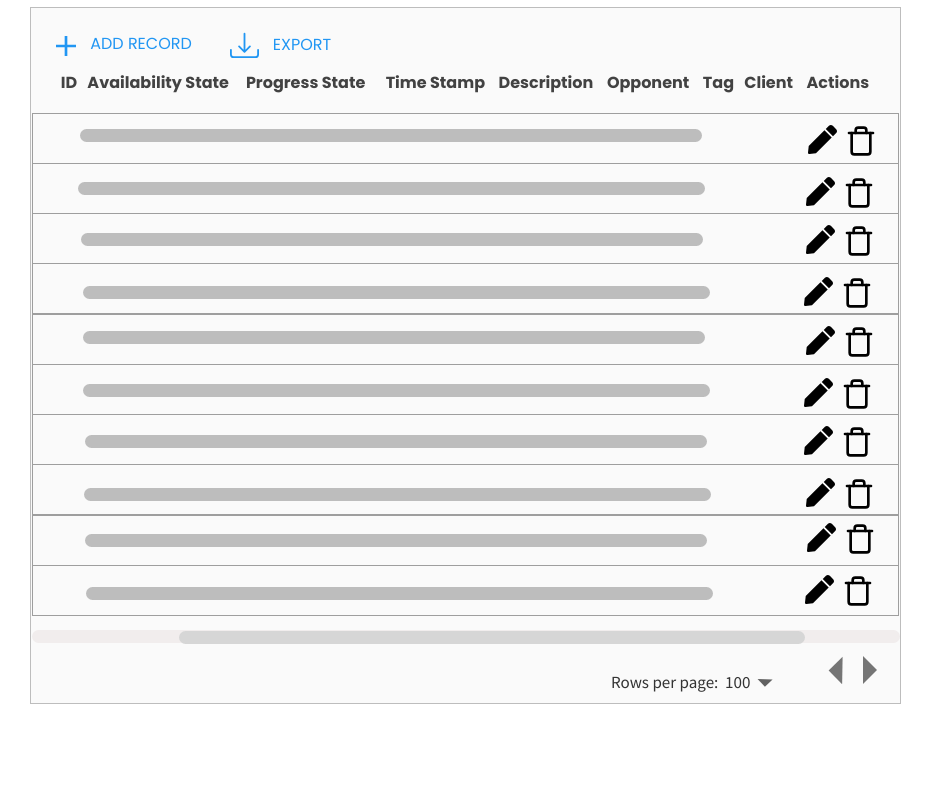
\includegraphics[width=1\linewidth]{fig/table-comment-gui.png}
\caption{Mockup de la Interfaz para las Tablas de Consultas}
\label{fig:table-consult-gui}
\end{figure}



\section{Requerimientos Funcionales}
Según Somerville \cite{Somerville}, Los requerimientos funcionaless son ``Son enunciados acerca de servicios que el sistema
debe proveer, de cómo debería reaccionar el sistema a entradas particulares y de cómo debería comportarse el sistema en situaciones específicas. En algunos casos, los requerimientos funcionales también explican lo que no debe hacer el sistema''

En el marco de este proyecto, los requerimientos funcionales se agrupan según sus funcionalidades específicas:

\begin{table}[H]
\centering
\begin{tabular}{|l|l|}
\hline
\textbf{Referencia} & \textbf{Función} \\
\hline
\textbf{RF.1} & Sistema de solicitudes de asignación de casos \\
\hline
\textbf{RF.2} & Sistema de gestión de casos por comisión \\
\hline
\textbf{RF.3} & Sistema de registro de clientes y consultas \\
\hline
\textbf{RF.4} & Sistema de alertas y notificaciones \\
\hline
\textbf{RF.5} & Registro y Autenticación de Usuarios \\
\hline
\end{tabular}
\caption{Requerimientos Funcionales}
\label{tab:rf}
\end{table}



\subsection{Sistema de Solicitudes de Asignación de Casos}

\begin{table}[H]
    \centering
    \begin{tabular}{|c|p{10cm}|}
        \hline
        \textbf{Referencia} & \textbf{Función} \\
        \hline
        RF.1.1 & Un Tomador de Caso podrá revisar la información de una consulta. \\
        \hline
        RF.1.2 & Un Tomador de Caso podrá revisar la cantidad de casos con sus estados de actividad de una comisión. \\
        \hline
        RF.1.3 & Un Tomador de Caso podrá revisar el historial reciente de solicitudes de una comisión. \\
        \hline
        RF.1.4 & Un Tomador de Caso podrá enviar una solicitud de asignación de un caso a una comisión. \\
        \hline
        RF.1.5 & Un Tomador de Caso podrá deshacer una solicitud de asignación. \\
        \hline
        RF.1.6 & Un Tomador de Caso podrá revisar la totalidad de casos. \\
        \hline
        RF.1.7 & Un Tomador de Caso podrá revisar la totalidad de clientes. \\
        \hline
    \end{tabular}
    \caption{Requerimientos Funcionales para Tomadores de Caso}
    \label{tab:rf-tomadores-caso}
\end{table}



\subsection{Sistema de Gestión de Casos por Comisión}
\begin{table}[H]
    \centering
    \begin{tabular}{|c|p{10cm}|}
        \hline
        \textbf{Requerimiento} & \textbf{Función} \\
        \hline
        RF.2.1 & Un usuario de una comisión tendrá la capacidad de aceptar o rechazar una solicitud de asignación de un nuevo caso a su comisión. \\
        \hline
        RF.2.2 & Un usuario de una comisión podrá visualizar los casos asignados a la comisión, incluyendo su estado y detalles relevantes. \\
        \hline
        RF.2.3 & Un usuario de una comisión podrá realizar modificaciones en los casos asignados a la comisión, actualizando la información según sea necesario. \\
        \hline
        RF.2.4 & Un usuario de una comisión podrá comentar en los casos asignados a la comisión, proporcionando información adicional o aclaraciones con la posibilidad de adjuntar archivos. \\
        \hline
        RF.2.5 & Un usuario de una comisión tendrá la opción de agregar y quitar eventos en los casos asignados a la comisión, permitiendo un seguimiento detallado de las actividades relacionadas con cada caso. \\
        \hline
    \end{tabular}
    \caption{Requerimientos Funcionales del Sistema de Gestión de Casos por Comisión}
    \label{tab:rf-gestion-casos-comision}
\end{table}

\subsection{Sistema de Registro de Clientes y Consultas}

\begin{table}[H]
    \centering
    \begin{tabular}{|l|p{10cm}|}
        \hline
        \textbf{Requerimiento} & \textbf{Descripción} \\
        \hline
        RF.3.1 & Un Tomador de Caso o Super Usuario podrá almacenar los datos de un cliente en el sistema. \\
        \hline
        RF.3.2 & Un Tomador de Caso o Super Usuario podrá registrar los detalles de una consulta de un cliente en el sistema. \\
        \hline
        RF.3.3 & El sistema permitirá cargar clientes mediante la integración con Google Forms, agilizando el ingreso de datos al sistema. \\
        \hline
        RF.3.4 & El sistema permitirá cargar consultas mediante la integración con Google Forms, facilitando el registro eficiente de información relacionada con las consultas de los clientes. \\
        \hline
    \end{tabular}
    \caption{Requerimientos del Sistema de Registro de Clientes y Consultas}
    \label{tab:registro-clientes-consultas}
\end{table}


\subsection{Sistema de Notificaciones y Alertas}

\begin{table}[H]
    \centering
    \begin{tabular}{|l|p{10cm}|}
        \hline
        \textbf{Requerimiento} & \textbf{Descripción} \\
        \hline
        RF.4.1 & El sistema podrá enviar correos electrónicos para notificar a los Tomadores de Caso cuando una solicitud es aceptada o rechazada. \\
        \hline
        RF.4.2 & El sistema podrá enviar correos electrónicos a los usuarios de una comisión al llegar una nueva solicitud de asignación de caso. \\
        \hline
        RF.4.3 & El sistema enviará alertas en tiempo real a los Tomadores de Caso cuando una solicitud es aceptada o rechazada. \\
        \hline
        RF.4.4 & El sistema enviará alertas a los usuarios de una comisión al llegar una solicitud de asignación de caso. \\
        \hline
        RF.4.5 & El sistema enviará alertas cuando ingresa un nuevo cliente o consulta a través de Google Forms, manteniendo a los usuarios informados sobre las actualizaciones en el sistema. \\
        \hline
    \end{tabular}
    \caption{Requerimientos del Sistema de Notificaciones y Alertas.}
    \label{tab:notificaciones-alertas}
\end{table}

\subsection{Registro y Autenticación de Usuarios}

\begin{table}[H]
    \centering
    \begin{tabular}{|l|p{10cm}|}
        \hline
        \textbf{Requerimiento} & \textbf{Descripción} \\
        \hline
        RF.5.1 & Un usuario podrá acceder a la plataforma mediante un nombre de usuario y contraseña. \\
        \hline
        RF.5.2 & Un usuario podrá registrarse en la plataforma a través de un proceso de autenticación vía correo electrónico. El acceso a la plataforma estará condicionado a la aceptación por parte de un usuario administrador. \\
        \hline
        RF.5.3 & Un usuario tendrá la capacidad de cambiar su contraseña en caso de olvidarla. \\
        \hline
        RF.5.4 & La plataforma permitirá a los usuarios visualizar únicamente las páginas para las cuales tengan permisos. \\
        \hline
    \end{tabular}
    \caption{Requerimientos de Registro y Autenticación de Usuarios.}
    \label{tab:registro-autenticacion}
\end{table}

\section{Requerimientos No Funcionales}
Según Somerville \cite{Somerville}, los requerimientos no funcionales son ``Son limitaciones sobre servicios o funciones que
ofrece el sistema. Incluyen restricciones tanto de temporización y del proceso de
desarrollo, como impuestas por los estándares. Los requerimientos no funcionales
se suelen aplicar al sistema como un todo, más que a características o a servicios
individuales del sistema.''

\begin{table}[H]
\centering
\begin{tabular}{|l|l|}
\hline
\textbf{Referencia} & \textbf{Función} \\
\hline
\textbf{RNF.1} & Requerimientos del producto \\
\hline
\textbf{RNF.2} & Requerimientos de la organización \\
\hline
\textbf{RNF.3} & Requerimientos externos \\
\hline
\end{tabular}
\caption{Requerimientos No Funcionales}
\label{tab:rnf}
\end{table}

\subsection{Requerimientos del producto}

\begin{table}[H]
    \centering
    \begin{tabular}{|l|p{10cm}|}
        \hline
        \textbf{Requerimiento} & \textbf{Descripción} \\
        \hline
        RNF.1.1 & El sistema se podrá acceder a través de la web desde una computadora con acceso a internet. \\
        \hline
        RNF.1.2 & La interfaz de usuario deberá ser intuitiva y fácil de usar, siguiendo los principios de diseño de experiencia de usuario (UX). \\
        \hline
        RNF.1.3 & El sistema deberá ser capaz de manejar simultáneamente por 5 a 10 usuarios sin degradación del rendimiento. \\
        \hline
        RNF.1.4 & El acceso a ciertas funcionalidades estará restringido a usuarios autorizados mediante roles y permisos. \\
        \hline
    \end{tabular}
    \caption{Requerimientos del Producto.}
    \label{tab:rnf-producto}
\end{table}

\subsection{Requerimientos de la organización}

\begin{table}[H]
    \centering
    \begin{tabular}{|l|p{10cm}|}
        \hline
        \textbf{Requerimiento} & \textbf{Descripción} \\
        \hline
        RNF.2.1 & La PC del usuario deberá tener un mínimo de 4GB de RAM y tarjeta de red para la conexión a internet. \\
        \hline
        RNF.2.2 & La plataforma será compatible con versiones estables de Chrome \(>=\) 120.0.6099.* y accesible a través de pantallas medianas a grandes. \\
        \hline
        RNF.2.3 & El código fuente deberá seguir buenas prácticas de desarrollo y ser fácilmente mantenible. \\
        \hline
    \end{tabular}
    \caption{Requerimientos de la Organización.}
    \label{tab:rnf-organizacion}
\end{table}

\subsection{Requerimientos externos}

\begin{table}[H]
    \centering
    \begin{tabular}{|l|p{10cm}|}
        \hline
        \textbf{Requerimiento} & \textbf{Descripción} \\
        \hline
        RNF.3.1 & Un usuario deberá aceptar los términos y condiciones para el registro a la plataforma. \\
        \hline
        RNF.3.2 & El sistema debe aplicar una política de complejidad de contraseñas que incluya la longitud mínima, uso de mayúsculas, minúsculas, números y caracteres especiales. \\
        \hline
        RNF.3.3 & Se debe implementar una protección efectiva contra ataques de fuerza bruta en las interfaces administrativas, incluyendo mecanismos de bloqueo temporal de cuentas. \\
        \hline
        RNF.3.4 & La integración con Google Forms y la API debe utilizar tokens de seguridad para autenticar y autorizar las solicitudes, manteniendo un flujo seguro de información. \\
        \hline
        RNF.3.5 & La plataforma deberá implementar medidas de seguridad contra ataques CSRF Token. \\
        \hline
        RNF.3.6 & La comunicación entre el servidor y los usuarios debe estar cifrada mediante un certificado SSL proporcionado por Let's Encrypt y configurado en el servidor Nginx. \\
        \hline
    \end{tabular}
    \caption{Requerimientos Externos.}
    \label{tab:rnf-externos}
\end{table}


\section{Definición de Roles y Responsabilidades}

\begin{table}[H]
    \centering
    \begin{tabular}{|p{3cm}|p{12cm}|}
        \hline
        \textbf{Tomador de Caso} & Este usuario tiene acceso al tablero de la consultoría y al panel de control. Su responsabilidad principal es agregar clientes y consultas de forma manual, además de asignar las consultas a una comisión específica. Los Tomadores de Caso pueden visualizar el estado de cada comisión, revisando la cantidad de casos activos y las últimas solicitudes enviadas.\\
        \hline
        \textbf{Integrante de Comisión (Profesor)} & Este rol se asigna a los integrantes de una comisión con acceso al tablero. Sus responsabilidades incluyen aceptar o rechazar solicitudes de asignación de casos o consultas. Además, se encargan de gestionar el seguimiento y progreso de cada caso asignado a su comisión.\\
        \hline
        \textbf{Jefe de Patrocinio (Administrador)} & También conocido como administrador, este usuario tiene privilegios que le otorgan acceso total a la plataforma. Sus responsabilidades principales incluyen la gestión de usuarios, permisos y roles, asegurando el correcto funcionamiento y la seguridad de la plataforma.\\
        \hline
        \textbf{Cliente (por Google Forms)} & Consultante que busca patrocinio gratuito. Este actor no tiene acceso directo a la plataforma y no ingresa a ella. Su interacción se limita a completar formularios de registro de cliente y consulta, los cuales se cargan automáticamente en la plataforma desde \textbf{Google Forms}.\\
        \hline

    \end{tabular}
    \caption{Roles y Responsabilidades de los Actores en la Plataforma}
    \label{tab:roles-responsabilidades}
\end{table}


\section{Diagrama de Caso de Uso del Sistema}
A continuación, se presentan los diagramas de caso de uso \ref{fig:caso-de-uso} para identificar a los actores implicados en una interacción. Si bien en este caso no se relacionan los casos de uso a alto nivel con diferentes actores, no significa que no exista una relación. Por otro lado, debe entenderse que Google Forms también cumple un rol e interactúa con el sistema principal Case Management System.

\begin{figure}[H]
\centering
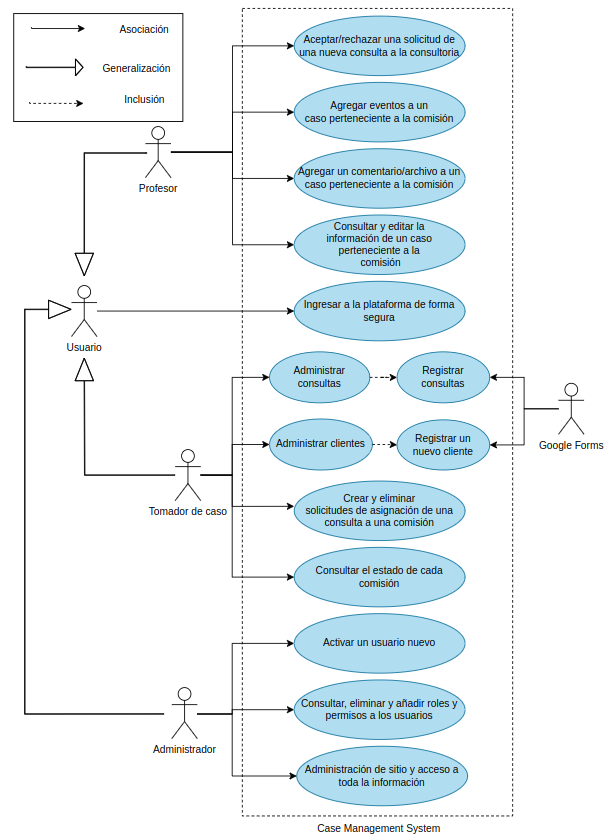
\includegraphics[width=1\linewidth]{fig/caso-de-uso.png}
\caption{Diagrama Caso de Uso}
\label{fig:caso-de-uso}
\end{figure}

\begin{itemize}
\item \textbf{CU.1}: Aceptar/rechazar una solicitud de una nueva consulta a la consultoría.
\item \textbf{CU.2}: Agregar eventos a un caso perteneciente a la comisión.
\item \textbf{CU.3}: Agregar un comentario/archivo a un caso perteneciente a la comisión.
\item \textbf{CU.4}: Ingresar a la plataforma de forma segura.
\item \textbf{CU.5}: Administrar consultas.
\item \textbf{CU.6}: Administrar clientes.
\item \textbf{CU.7}: Crear y eliminar solicitudes de asignación de una consulta a una comisión.
\item \textbf{CU.8}: Ver el estado de cada comisión.
\item \textbf{CU.9}: Activar a un usuario nuevo.
\item \textbf{CU.10}: Administrar roles y permisos de los usuarios.
\item \textbf{CU.11}: Administración de sitio y acceso a toda la información.
\end{itemize}


\section{Diagrama de Secuencia Nominal Simplificado}
A continuación, se incluye un diagrama de secuencia \ref{fig:secuencia-nominal} simplificado de alto nivel que representa una secuencia nominal para agregar comprensión a la funcionalidad de cada actor y su interacción con otros actores.

\begin{figure}[H]
\centering
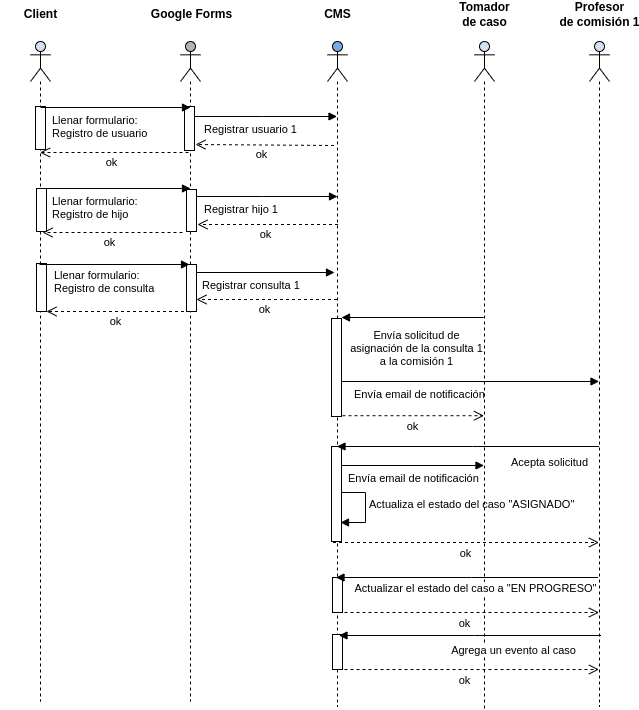
\includegraphics[width=1\linewidth]{fig/secuencia-basica.png}
\caption{Diagrama de Secuencia Simplificado}
\label{fig:secuencia-nominal}
\end{figure}

En este diagrama, participan varios actores, incluyendo un cliente con un solo hijo, el sistema externo Google Forms, el sistema Case Management System, el usuario tomador de caso, el profesor de la comisión número uno y el jefe de patrocinio o administrador.

Además, se detallan dos eventos en paralelo: el registro de un usuario en la plataforma y el registro de un cliente con una nueva consulta.

\section{Matriz de Trazabilidad}
La siguiente matriz de trazabilidad relaciona cada uno de los requerimientos con los casos de uso.

\begin{table}[H]
    \centering
    \small
    \begin{tabular}{|c|@{}c|@{}c|@{}c|@{}c|@{}c|@{}c|@{}c|@{}c|@{}c|@{}c|@{}c|}
    \hline
               & \textbf{CU1} & \textbf{CU2} & \textbf{CU3} & \textbf{CU4} & \textbf{CU5} & \textbf{CU6} & \textbf{CU7} & \textbf{CU8} & \textbf{CU9} & \textbf{CU10} & \textbf{CU11}\\
    \hline
    \hline
        \textbf{RF.1.1} &  &  & & &  & $\bullet$&  &  &  & & \\
        \hline
        \textbf{RF.1.2} &  &  & & &  &  &  &  & $\bullet$ & & \\
        \hline
        \textbf{RF.1.3} &  &  & &  &  &  &  &  & $\bullet$ & & \\
        \hline
        \textbf{RF.1.4} &  &  & &  &  &  &  & $\bullet$ &  & & \\
        \hline
        \textbf{RF.1.5} &  &  & &  &  &  &  & $\bullet$ &  & & \\
        \hline
        \textbf{RF.1.6} &  &  & &  &  & $\bullet$ &  &  &  & & \\
        \hline
        \textbf{RF.1.7} &  &  & &  &  &  &  $\bullet$ &  &  & & \\
        \hline
        \textbf{RF.2.1} & $\bullet$ &  &  & &  &  &  &  &  & & \\
        \hline
        \textbf{RF.2.2} &  &  &  & & $\bullet$ &  &  &  &  & & \\
        \hline
        \textbf{RF.2.3} &  &  & & & $\bullet$ &  &  &  &  & & \\
        \hline
        \textbf{RF.2.4} &  &  & $\bullet$ & & &  &  &  &  & & \\
        \hline
        \textbf{RF.2.5} &  & $\bullet$ &  & & &  &  &  &  & & \\
        \hline
        \textbf{RF.3.1} &  &  &  & &  &  & $\bullet$ &  &  & & $\bullet$ \\
        \hline
        \textbf{RF.3.2} &  &  &  & & & $\bullet$ &  &  &  & & $\bullet$ \\
        \hline
        \textbf{RF.3.3} &  &  &  & & &  & $\bullet$ &  &  & & \\
        \hline
        \textbf{RF.3.4} &  &  &  & & & $\bullet$ &  &  &  & & \\
        \hline
        \textbf{RF.4.1} & $\bullet$ & & &  &  &  &  &  &  & & \\
        \hline
        \textbf{RF.4.2} &  &  & & &  &  &  & $\bullet$ &  & & \\
        \hline
        \textbf{RF.4.3} & $\bullet$ &  & &  &  &  &  &  &  & & \\
        \hline
        \textbf{RF.4.4} &  &  &  & &  &  &  & $\bullet$ &  & & \\
        \hline
        \textbf{RF.4.5} &  &  &  & & &  & $\bullet$ &  &  & & \\
        \hline
        \textbf{RF.5.1} &  &  &  & $\bullet$ & &  &  &  &  & & \\
        \hline
        \textbf{RF.5.2} &  &  &  & $\bullet$ & &  &  &  & & & \\
        \hline
        \textbf{RF.5.3} &  &  &  & $\bullet$ &  &  &  &  &  & & \\
        \hline
        \textbf{RF.5.4} &  &  &  &&  &  &  &  &  & $\bullet$ & \\
    \hline
        \textbf{RNF.1.1} &  &  & & &  &  &  &  &  & & \\
        \hline
        \textbf{RNF.1.2} &  &  & & &  &  &  &  &  & & \\
        \hline
        \textbf{RNF.1.3} &  &  & & &  &  &  &  &  & & \\
        \hline
        \textbf{RNF.1.4} &  &  & & &  &  &  &  &  & $\bullet$ & \\
        \hline
        \textbf{RNF.2.1} &  &  & & &  &  &  &  &  & & \\
        \hline
        \textbf{RNF.2.2} &  &  & & &  &  &  &  &  & & \\
        \hline
        \textbf{RNF.2.3} &  &  & & &  &  &  &  &  & & \\
        \hline
        \textbf{RNF.3.1} &  &  & & &  &  &  &  &  & & \\
        \hline
        \textbf{RNF.3.2} &  &  &&  &  &  &  &  &  & & \\
        \hline
        \textbf{RNF.3.3} &  &  & & &  &  &  &  &  & & \\
        \hline
        \textbf{RNF.3.4} &  &  & & &  &  &  &  &  & & \\
        \hline
        \textbf{RNF.3.5} &  &  & & &  &  &  &  &  & & \\
        \hline
        \textbf{RNF.3.6} &  &  &  & &  &  &  &  &  & & \\
    \hline
    \end{tabular}
    \caption{Matriz de Trazabilidad}
    \label{tab:matriz-trazabilidad}
\end{table}


    \chapter{Despliegue y Operación}\label{cap:sum}

\section{Introducción}
Este capítulo aborda el proceso integral de instalación y puesta en marcha del servicio, detallando el despliegue de la pila de contenedores en Swarm. Además, se proporciona una guía práctica sobre el uso efectivo de la misma.


\section{Instalación de la Plataforma}

Para iniciar el proceso de instalación, es necesario contar con el repositorio de deploy. Puede clonar el repositorio desde GitHub utilizando el siguiente comando:


%estilo de comando
\lstdefinestyle{consola} {
    numbers=none,
    xleftmargin=\parindent,
    xrightmargin=\parindent,
    aboveskip=3mm,
    belowskip=0.01mm,
    basicstyle=\small\bf\ttfamily,
    backgroundcolor=\color{black!08},
}


\begin{lstlisting}[style=consola]
$ git clone git@github.com:proyecto-patrocinio/proyecto-patrocinio.git
\end{lstlisting}

Una vez clonado el repositorio, es fundamental realizar la configuración previa de los archivos.
 A continuación, se proporciona una descripción detallada de los archivos de configuración del repositorio de deploy. 

\lstset{
  basicstyle=\ttfamily,
  breaklines=true,
  postbreak=\mbox{\textcolor{red}{$\hookrightarrow$}\space},
}

\begin{lstlisting}
.
|-- .env
|-- docker-compose.yml
|-- dotenv.sh
|-- README.md
|-- resources
|   |-- backend.env
|   |-- frontend.env
|   |-- nginx.conf
|   |-- postgres.env
|   |-- templates
|   |   |-- account
|   |   |   |-- email_confirmation_message.html
|   |   |   |-- email_confirmation_signup_message.html
|   |   |-- notifications
|   |   |   |-- new_request.html
|   |   |   |-- request_accepted.html
|   |   |   |-- request_rejected.html
|   |-- terms_and_policies.md
\end{lstlisting}




\subsection{Configuración de Templates}
\begin{enumerate}
    \item En la carpeta \texttt{\textbf{templates/account}}, se encuentran los siguientes templates:

\begin{itemize}
    \item \texttt{email\_confirmation\_signup\_message}: HTML enviado por email en la confirmación del registro de una cuenta.
    \item \texttt{email\_confirmation\_message}: HTML enviado por email cuando se solicita reenviar el email para el registro de usuario.
    \item \texttt{password\_reset\_key\_message}: HTML enviado por email cuando se solicitó cambiar contraseña olvidada.
\end{itemize}


 \item  En la carpeta \texttt{\textbf{templates/notifications}}, se encuentran los siguientes templates:

\begin{itemize}
    \item \texttt{new\_request}: HTML enviado por email para notificar al usuario cuando la comisión tiene una nueva solicitud de asignación de caso.
    \item \texttt{request\_accepted}: HTML enviado por email en la notificación al tomador de caso cuando una comisión aceptó una solicitud.
    \item \texttt{request\_rejected}: HTML enviado por email en la notificación al tomador de caso cuando una comisión rechazó una solicitud.
\end{itemize}


\end{enumerate}



\subsection{Configuración de Variables de Entorno en el Archivo \texttt{.env}}

En el archivo \texttt{.env}, se deben establecer las siguientes variables de entorno que serán reenderizadas por el archivo compose \textit{docker-compose.yml}. A continuación, se presenta una tabla con descripciones de cada variable:

\begin{table}[H]
    \centering
    \begin{tabular}{|l|p{7cm}|}
    \hline
    \textbf{Variable de Entorno} & \textbf{Descripción} \\
    \hline
    CMS\_BACKEND\_IMAGE & Nombre de la imagen de Docker para el backend. \\
    \hline
    CMS\_FRONTEND\_IMAGE & Nombre de la imagen de Docker para el frontend.\\
    \hline
    CMS\_PROXY\_PORT & Puerto del servidor proxy Nginx. \\
    \hline
    CMS\_NGINX\_CONFIG\_FILE & Ruta al archivo de configuración de NGINX. \\
    \hline
    CMS\_BACKEND\_ENV\_FILE & Ruta al archivo de variables de entorno para el backend. \\
    \hline
    CMS\_POSTGRES\_ENV\_FILE & Ruta al archivo de variables de entorno para PostgreSQL. \\
    \hline
    CMS\_FRONTEND\_ENV\_FILE & Ruta al archivo de variables de entorno para el frontend. \\
    \hline
    CMS\_TEMPLATES\_ACCOUNT\_PATH & Ruta al directorio de plantillas de ``account''. \\
    \hline
    CMS\_TEMPLATES\_NOTIFICATION\_PATH & Ruta al directorio de plantillas de ``notifications''.\\
    \hline
    CMS\_TERMS\_AND\_POLICIES\_FILE & Ruta al archivo de términos y políticas. \\
    \hline
    \end{tabular}
    \caption{Configuración de Variables de Entorno en el Archivo \texttt{.env}}
    \label{tab:env-file-variables}
\end{table}

Consulte el anexo para revisar las variables utilizadas: \ref{sec:anexo:configfile-env}.


\subsection{Configuración de Variables de Entorno en \texttt{backend.env}}

En el archivo \texttt{\textbf{backend.env}}, se deben configurar las siguientes variables de entorno. A continuación, se presenta una tabla con descripciones de cada variable:

\begin{table}[H]
    \centering
    \begin{tabular}{|l|p{7cm}|}
    \hline
    \textbf{Variable de Entorno} & \textbf{Descripción} \\
    \hline
    DEBUG & Modo de depuración (0 para desactivado, 1 para activado). \\
    \hline
    DJANGO\_ALLOWED\_HOSTS & Lista de hosts permitidos separados por espacios. \\
    \hline
    SQL\_ENGINE & Motor de base de datos para Django. Por ejemplo para postgres es `django.db.backends.postgresql'.\\
    \hline
    SQL\_DATABASE & Nombre de la base de datos. \\
    \hline
    SQL\_USER & Usuario de la base de datos. \\
    \hline
    SQL\_PASSWORD & Contraseña de la base de datos. \\
    \hline
    SQL\_HOST & Dirección del servidor de base de datos. \\
    \hline
    SQL\_PORT & Puerto del servidor de base de datos. \\
    \hline
    DATABASE & Tipo de base de datos. En este caso es `postgres'.\\
    \hline
    EMAIL\_HOST\_USER & Usuario del servidor de correo electrónico. \\
    \hline
    EMAIL\_HOST\_PASSWORD & Contraseña del servidor de correo electrónico. \\
    \hline
    CORS\_ALLOWED\_ORIGINS & Lista de orígenes permitidos para CORS. \\
    \hline
    HOSTNAME & Nombre del host de la aplicación. \\
    \hline
    CONSULTANCY\_BOARD\_NAME & Nombre de la comisión de consultoría. \\
    \hline
    DEFAULT\_HTTP\_PROTOCOL & Protocolo HTTP. \\
    \hline
    CSRF\_TRUSTED\_ORIGINS & Lista de orígenes confiables para CSRF. \\
    \hline
    LOG\_ROTATE\_DAYS & Días antes de rotar los archivos de log. \\
    \hline
    SECRET\_KEY & Clave secreta de Django. \\
    \hline
    DJANGO\_SUPERUSER\_USERNAME & Nombre de usuario del superusuario administrador para acceder a la web admin de Django. \\
    \hline
    DJANGO\_SUPERUSER\_PASSWORD & Contraseña del superusuario administrador del proyecto. \\
    \hline
    DJANGO\_SUPERUSER\_EMAIL & Correo electrónico del superusuario administrador. \\
    \hline
    \end{tabular}
    \caption{Configuración de Variables de Entorno en \texttt{backend.env}}
    \label{tab:env-variables}
\end{table}


Consulte el anexo para revisar las variables utilizadas: \ref{sec:anexo:configfile-backend-env}.


\subsection{Configuración de Variables de Entorno en \texttt{frontend.env}}

En el archivo \texttt{frontend.env}, se deben configurar las siguientes variables de entorno. A continuación, se presenta una tabla con descripciones de cada variable:

\begin{table}[H]
    \centering
    \begin{tabular}{|p{7cm}|p{7cm}|}
    \hline
    \textbf{Variable de Entorno} & \textbf{Descripción} \\
    \hline
    REACT\_APP\_URL\_BASE\_API
    \_REST\_PATROCINIO & URL base de la API REST de Patrocinio. Ejemplo https://\{\{dominio\}\}/api/. \\
    \hline
    REACT\_APP\_WS\_NOTIFICATION
    \_PATH\_PATROCINIO & Ruta del servidor asincrónico para notificaciones. Ejemplo wss://\{\{dominio\}\}/ws/notification/\\
        \hline
    \end{tabular}
    \caption{Configuración de Variables de Entorno en \texttt{frontend.env}}
    \label{tab:frontend-env-variables}
\end{table}
El resto de variables de entorno de este archivo no deben tocarse, son específicas para acceder a los endpoints del backend.

Consulte el anexo para revisar las variables utilizadas: \ref{sec:anexo:configfile-frontend-env}.



\subsection{Configuración de Variables de Entorno para la Base de Datos}

En el archivo \texttt{\textbf{backend.env}}, se deben configurar las siguientes variables de entorno relacionadas con la base de datos. A continuación, se presenta una tabla con descripciones de cada variable:

\begin{table}[H]
    \centering
    \begin{tabular}{|l|p{9cm}|}
    \hline
    \textbf{Variable de Entorno} & \textbf{Descripción} \\
    \hline
    POSTGRES\_DB & Nombre de la base de datos de Patrocinio en PostgreSQL. \\
    \hline
    POSTGRES\_USER & Usuario de la base de datos de Patrocinio en PostgreSQL. \\
    \hline
    PGDATA & Ruta del directorio de datos de PostgreSQL. \\
    \hline
    POSTGRES\_PASSWORD & Contraseña para el usuario de la base de datos de Patrocinio en PostgreSQL. \\
    \hline
    \end{tabular}
    \caption{Configuración de Variables de Entorno para la Base de Datos}
    \label{tab:database-env-variables}
\end{table}


Consulte el anexo para revisar las variables utilizadas: \ref{sec:anexo:configfile-portgres-env}.

\subsection{Archivo de Configuración de Nginx}

El archivo de configuración de Nginx puede obtener más información detallada en la sección correspondiente (\ref{subsec:nginx_explicacion}). Asegúrese de revisar esa sección para comprender y ajustar la configuración de Nginx según sea necesario para el correcto funcionamiento de la plataforma.

\subsection{Archivo \texttt{terms\_and\_policies}}

El archivo \texttt{terms\_and\_policies} debe configurarse según las políticas y términos que la plataforma desea establecer y que los usuarios deberán aceptar. Este archivo es crucial para definir las reglas y condiciones de uso de la plataforma.


\section{Despliegue de la Plataforma}

Para llevar a cabo el despliegue de la plataforma, se deben seguir los pasos detallados en el archivo README del repositorio de deploy.

Hasta la fecha actual, se dispone de un único nodo, que también actúa como nodo maestro, en el cual se ha implementado el despliegue mediante Docker Swarm. Este nodo maestro hospeda todos los servicios necesarios para la plataforma.

Inicialmente, el servidor ya contaba con un servidor Nginx en funcionamiento y un servicio de R Studio. Se procedió a integrar el servicio Case Management System en el servidor Nginx existente.

En la Figura \ref{fig:deploy-in-server} se presenta un diagrama que ilustra los servicios proporcionados por el servidor, destacando la composición del servicio Case Management System, definido a través de un Docker Stack.



Es importante tener en cuenta que si se decide agregar nodos adicionales al clúster de Docker Swarm, será necesario actualizar el controlador de volúmenes de Docker Swarm. Esto se realiza para permitir el intercambio de volúmenes entre los diferentes nodos del clúster.

\begin{figure}[H]
\centering
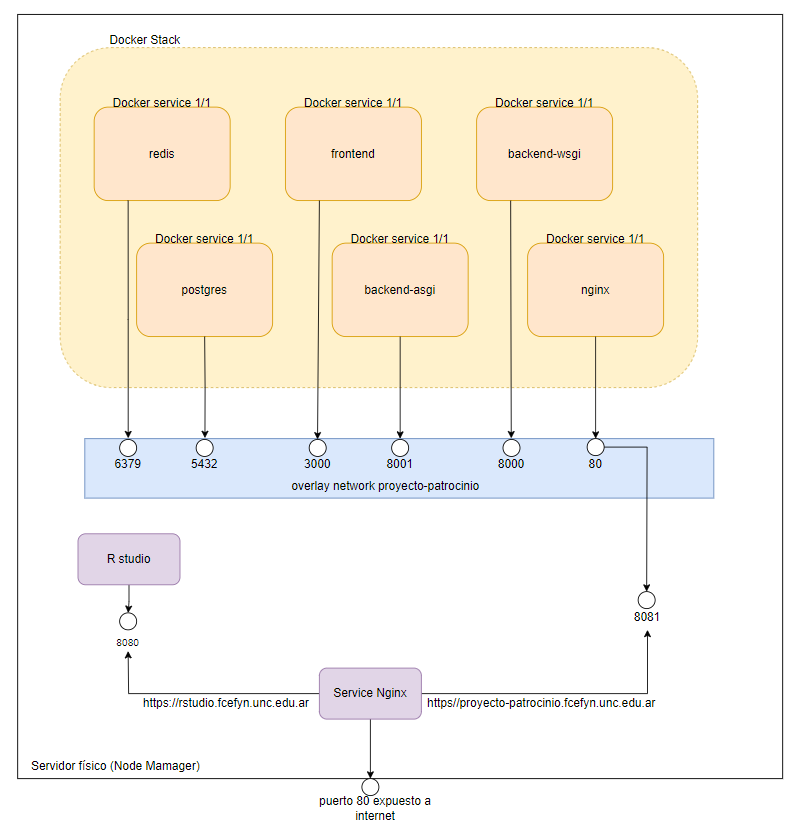
\includegraphics[width=1\linewidth]{fig/deploy.png}
\caption{Diagrama de Despliegue}
\label{fig:deploy-in-server}
\end{figure}

\section{Configuración}

Una vez que la plataforma esté en funcionamiento, el administrador debe acceder al panel web utilizando las credenciales proporcionadas en el archivo de configuración. A continuación, se describen los pasos para realizar la configuración inicial:

\begin{enumerate}
    \item Inicie sesión en la plataforma como administrador.
    \item Ingrese a la siguiente URL: \url{http://{{dominio}}/admin}.
    
    \item Verifique la configuración del dominio en la sección de sitios (Figura \ref{fig:config-sites}). Es esencial asegurarse de que el dominio esté correctamente establecido. Si es necesario realizar cambios, es \textbf{importante}\textbf{ no crear nuevos sitios ni eliminar} el existente, sino editar la información del sitio existente.
\end{enumerate}

\begin{figure}[H]
    \centering
    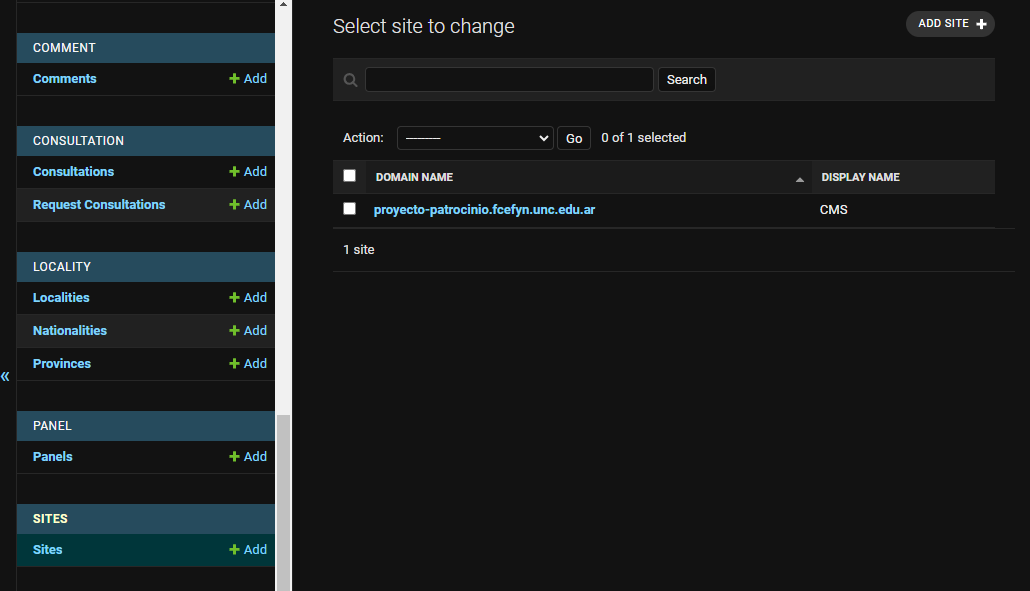
\includegraphics[width=1\linewidth]{fig/sites.png}
    \caption{Configuración de Sitios en el Panel de Administración.}
    \label{fig:config-sites}
\end{figure}


A continuación, el administrador debe crear todas las pizarras de trabajo para cada comisión existente en el patrocinio a través de la sección de \textit{Boards}.

\begin{figure}[H]
    \centering
    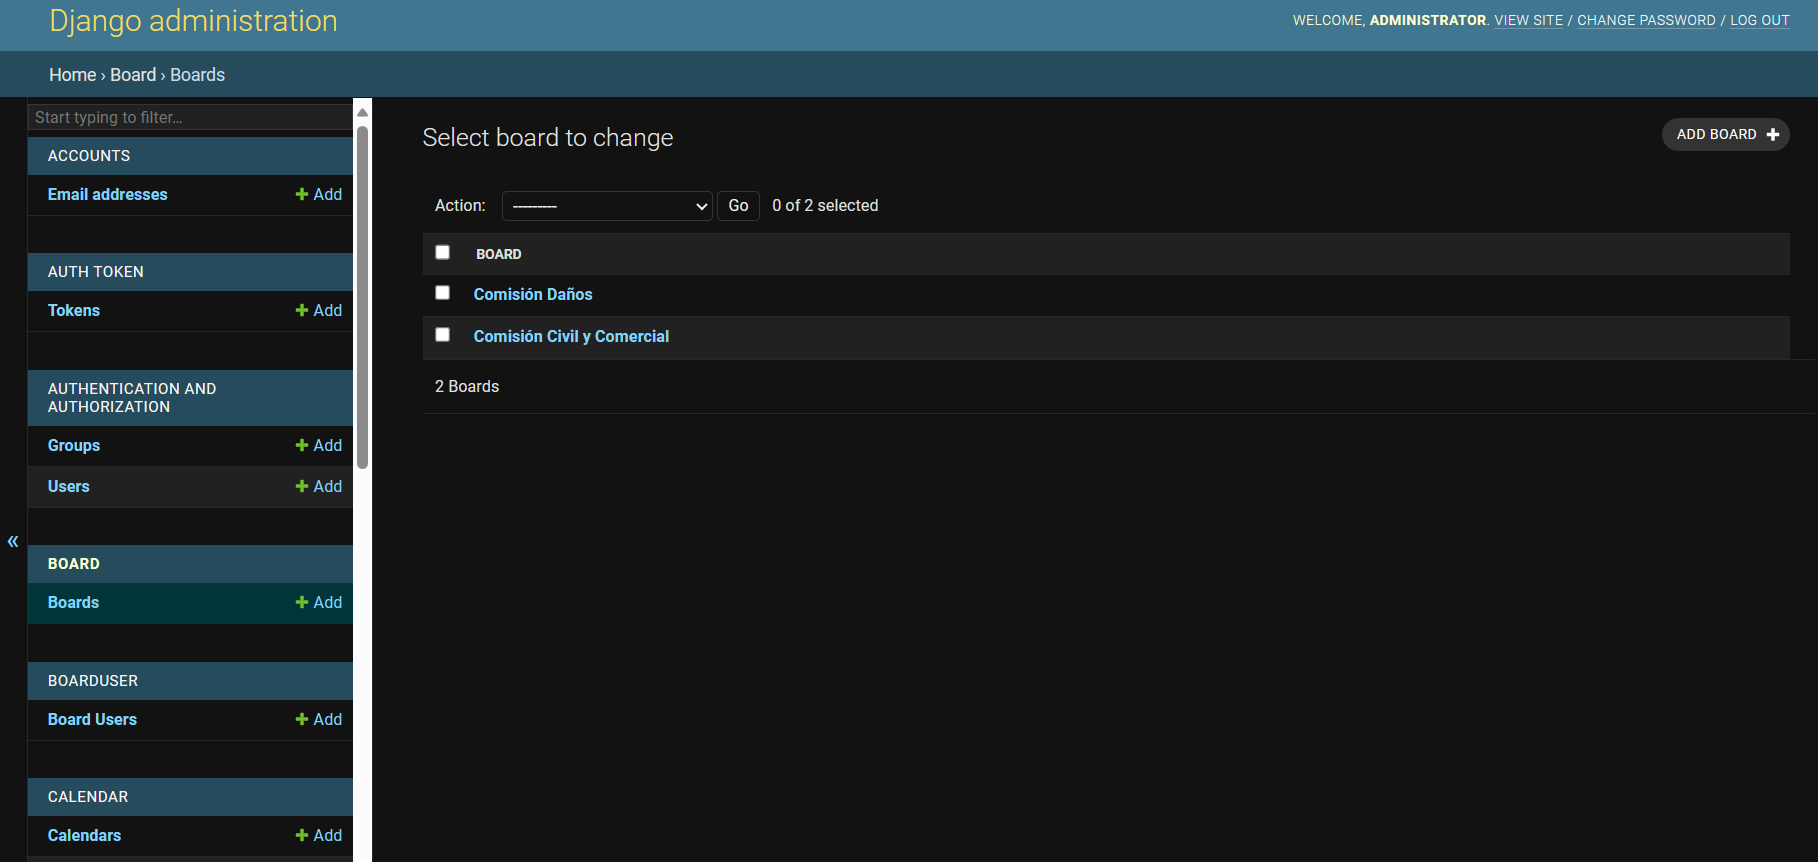
\includegraphics[width=1\linewidth]{fig/boards-admin.png}
    \caption{Creación de Pizarras en la Sección de Administración.}
    \label{fig:boards-admin}
\end{figure}

Finalmente, se deberá registrar una cuenta de usuario para la integración con Google Forms y otorgarle permisos de ``forms''. Para obtener información detallada sobre cómo realizar estos pasos, consulte la sección \ref{sec:registrar-cuenta} para la creación de la cuenta y la sección \ref{subsec:integracion-google-form} para la integración de la cuenta con Google Forms.



\section{Registro de Usuarios}\label{sec:registrar-cuenta}

Para poder registrar un usuario, El usuario deberá seguir los siguientes pasos:

\begin{enumerate}
    \item Ingresar a la página web y seleccionar la opción ``Don't have an account? Sign Up''.
    \item Completar los datos requeridos, acepte los términos y condiciones, y haga clic en el botón ``Sign up''.


    \begin{figure}[H]
        \centering
        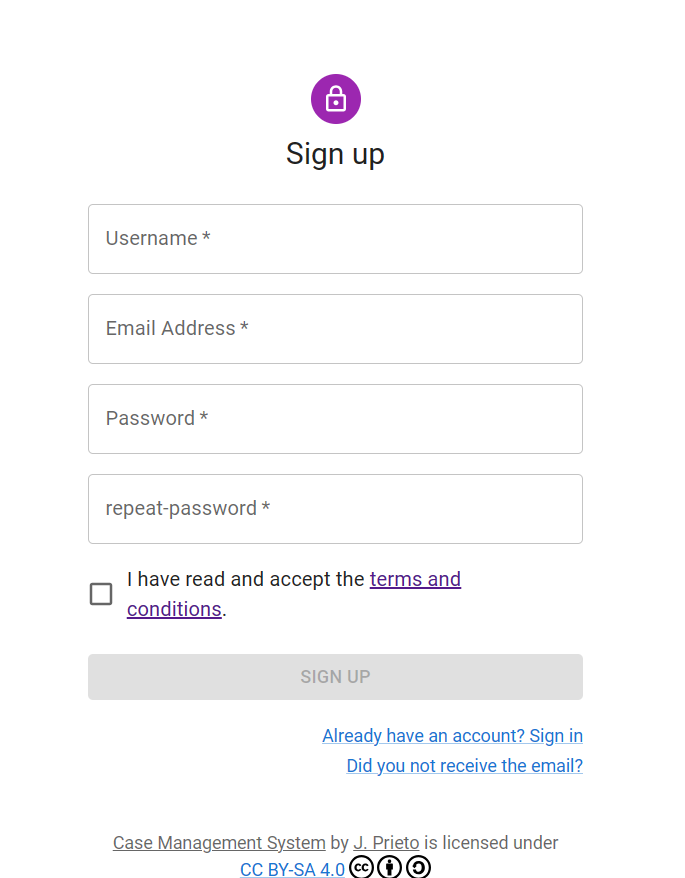
\includegraphics[width=0.7\linewidth]{fig/signup.png}
        \caption{Pantalla de Registro de Usuarios.}
        \label{fig:signup}
    \end{figure}

    \item Revisar la casilla de correlo electrónico y seleccionar el enlace en el correo enviado.

    \textbf{Nota}: El formato de este email, fue previamente configurado con los templates en la etapa de configuración de software.

    \begin{figure}[H]
        \centering
        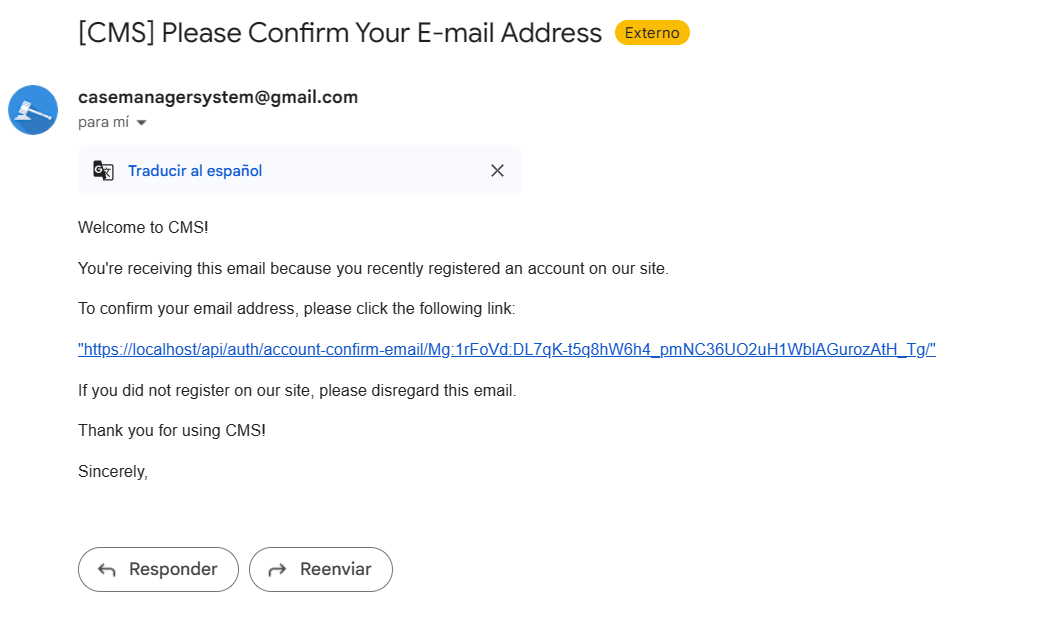
\includegraphics[width=1\linewidth]{fig/confirm-email.png}
        \caption{Confirmación por Correo Electrónico.}
        \label{fig:confirm-email}
    \end{figure}
\end{enumerate}
La página lo redirigirá a la principal, pero aún el usuario no podrá acceder hasta que un administrador habilite su cuenta. Para activar la cuenta, el administrador debe seguir estos pasos:

\begin{enumerate}
    \item Ingresar a la sección de administración y dirigirse a la pestaña de usuarios.
    \item Seleccionar el nuevo usuario y editar la sección de permisos.


    \begin{figure}[H]
        \centering
        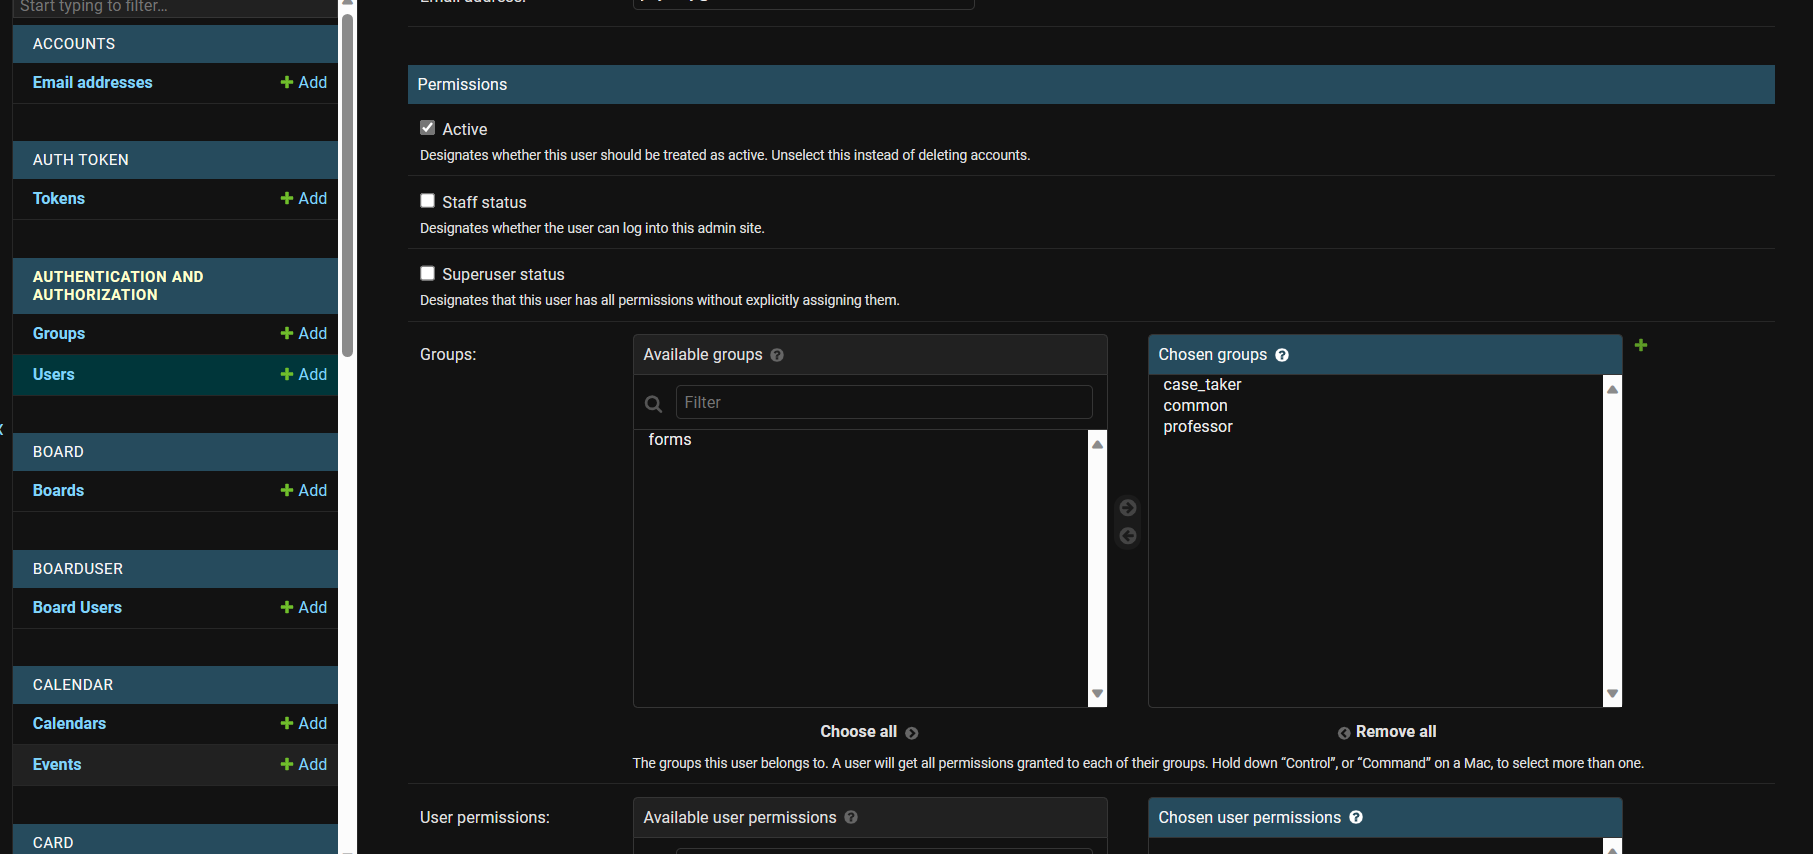
\includegraphics[width=1\linewidth]{fig/user-permission.png}
        \caption{Configuración de Permisos de Usuario.}
        \label{fig:user-permission}
    \end{figure}
    
    \item En la sección, marcar la opción ``Active'' y otorgar los permisos necesarios (ver \ref{sec:permisos-usuarios}) antes de guardar.

\end{enumerate}

Si el usuario es un miembro de una comisión, el administrador también deberá realizar los siguientes pasos adicionales.

\begin{enumerate}
    \item Ingresar a la sección ``Board Users''.
    \item Crear la relación del usuario con la comisión correspondiente.

    \begin{figure}[H]
        \centering
        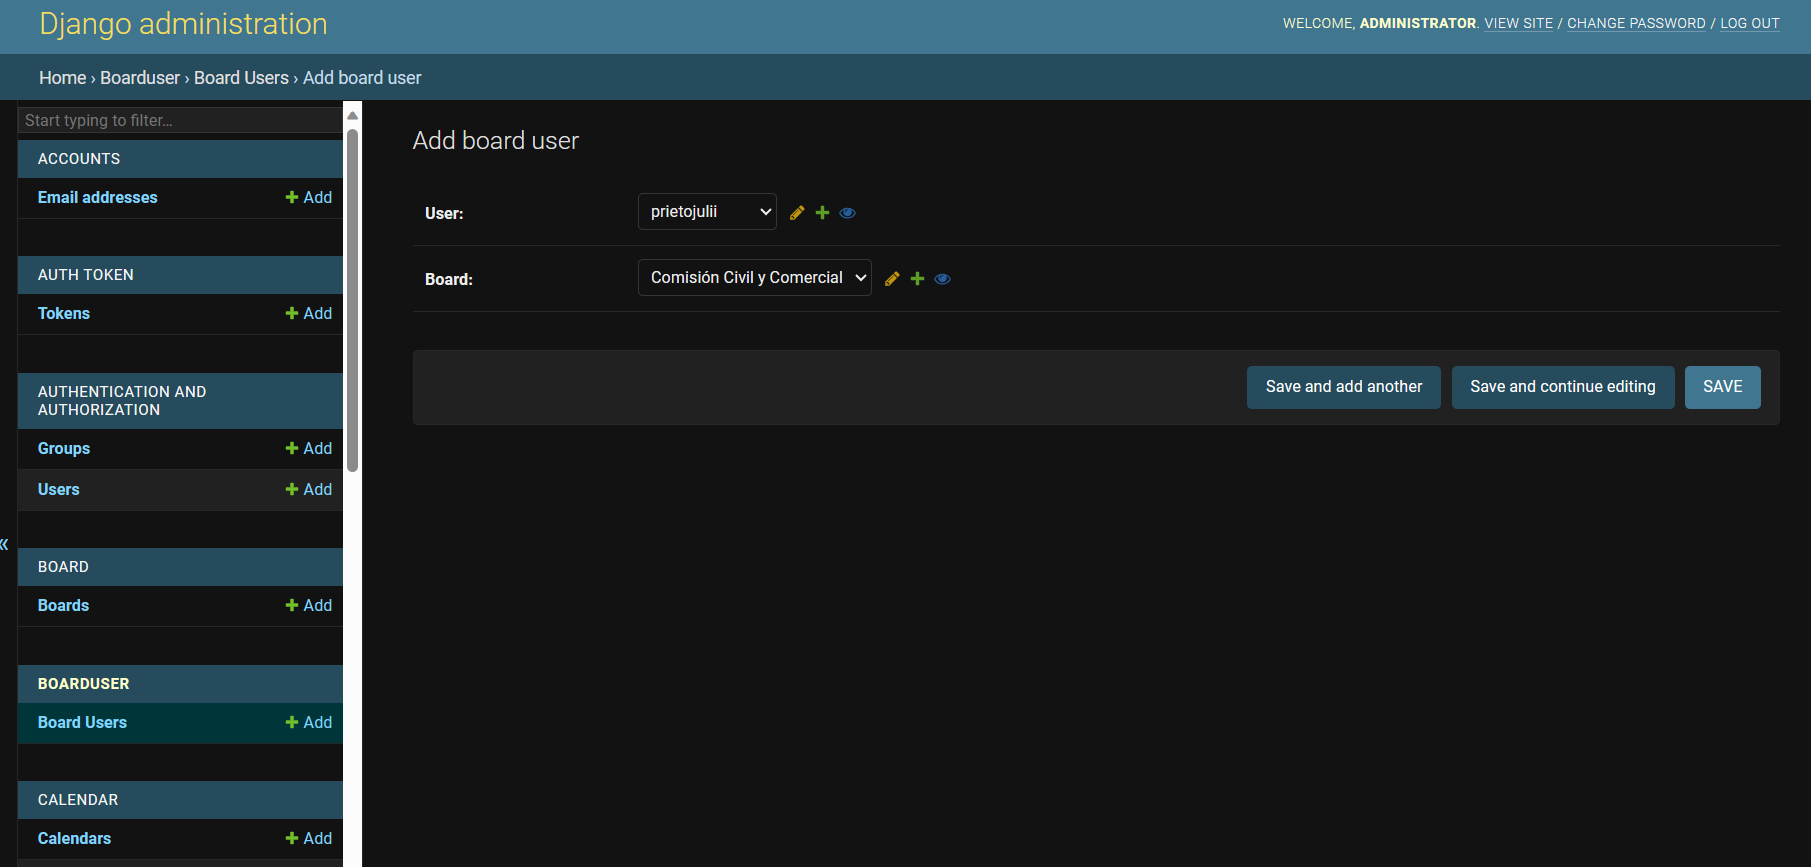
\includegraphics[width=1\linewidth]{fig/board-user.png}
        \caption{Creación de Relación Usuario-Comisión.}
        \label{fig:board-user}
    \end{figure}
    
    \begin{figure}[H]
        \centering
        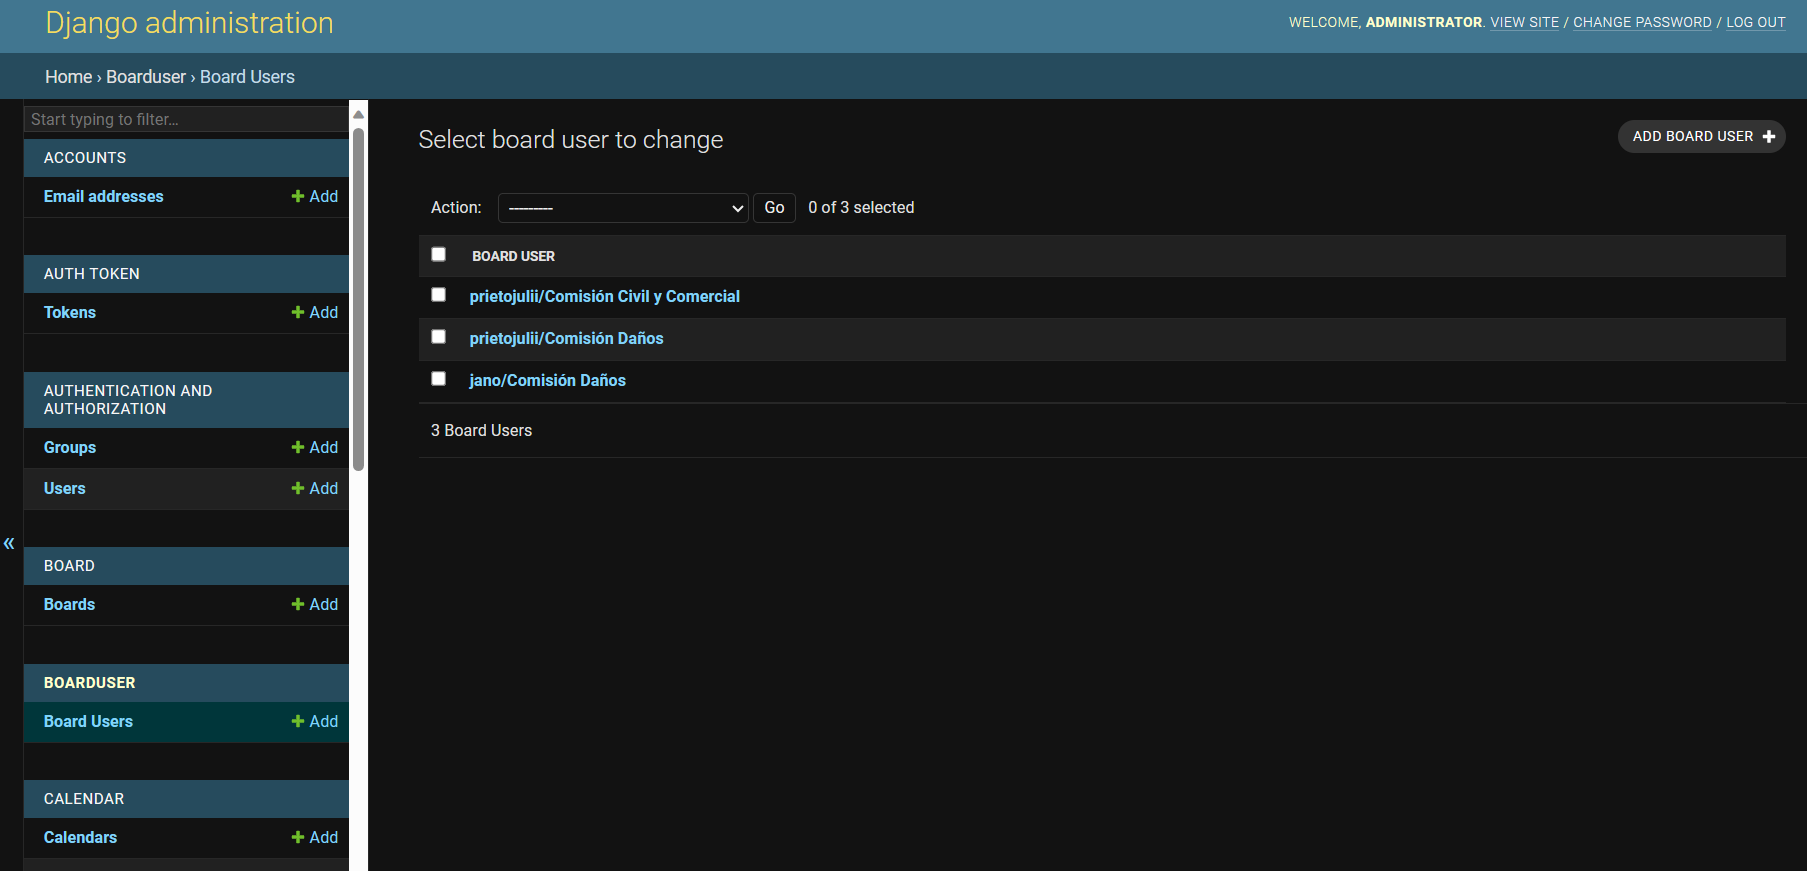
\includegraphics[width=1\linewidth]{fig/board-user-2.png}
        \caption{Lista de Relaciones Usuario-Comisión.}
        \label{fig:board-user-2}
    \end{figure}
\end{enumerate}

Después de completar estos pasos, el usuario podrá iniciar sesión correctamente en la web desde la página de inicio de sesión.

\begin{figure}[H]
    \centering
    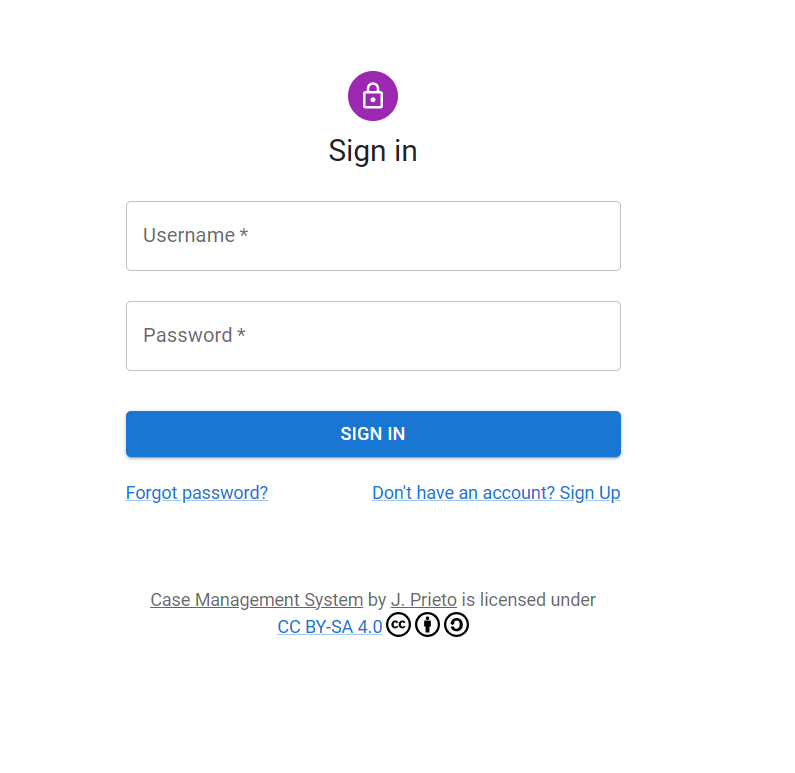
\includegraphics[width=0.7\linewidth]{fig/signin-real-page.png}
    \caption{Página de Inicio de Sesión.}
    \label{fig:signin-real-page-2}
\end{figure}



\section{Permisos de Usuario}\label{sec:permisos-usuarios}

Los grupos de permisos de usuarios se encuentran en la sección "Groups" de la página de administración y se detallan a continuación:

\begin{table}[H]
    \centering
    \begin{tabular}{|c|p{10cm}|}
        \hline
        \textbf{Grupo} & \textbf{Descripción}\\
        \hline
        common & Grupo de permisos básicos necesarios tanto para un tomador de caso como para un profesor.\\
        \hline
        case\_taker & Grupo de permisos para un tomador de caso. Necesarios para el manejo de la consultoría.\\
        \hline
        professor & Grupo de permisos para un profesor. Necesarios para el manejo de una comisión.\\
        \hline
        forms & Grupo de permisos exclusivo para la cuenta de Google Forms, que le permite registrar formularios.\\
        \hline
    \end{tabular}
    \caption{Grupos de Permisos de Usuario.}
    \label{tab:grupos-permisos-usuario}
\end{table}

\section{Permisos de Usuario}\label{sec:permisos-usuarios}

Los grupos de permisos de usuarios se encuentran en la sección "Groups" de la página de administración y se detallan a continuación:

\begin{table}[H]
    \centering
    \begin{tabular}{|c|p{10cm}|}
        \hline
        \textbf{Grupo} & \textbf{Descripción}\\
        \hline
        common & Grupo de permisos básicos necesarios tanto para un tomador de caso como para un profesor.\\
        \hline
        case_taker & Grupo de permisos para un tomador de caso. Necesarios para el manejo de la consultoría.\\
        \hline
        professor & Grupo de permisos para un profesor. Necesarios para el manejo de una comisión.\\
        \hline
        forms & Grupo de permisos exclusivo para la cuenta de Google Forms, que le permite registrar formularios.\\
        \hline
    \end{tabular}
    \caption{Grupos de Permisos de Usuario.}
    \label{tab:grupos-permisos-usuario}
\end{table}

\textbf{Nota:} El grupo de permisos \textit{common} debe asignarse junto con \textit{case\_taker} o \textit{professor}.


\section{Administración}\label{sec:administracion}

La página de administración proporciona una interfaz amigable para visualizar y gestionar todos los datos del sistema. Al ingresar a la página principal, se presenta una disposición organizada de los datos agrupados en secciones. Además, a la derecha, se muestra un historial de acciones recientes.

\begin{figure}[H]
    \centering
    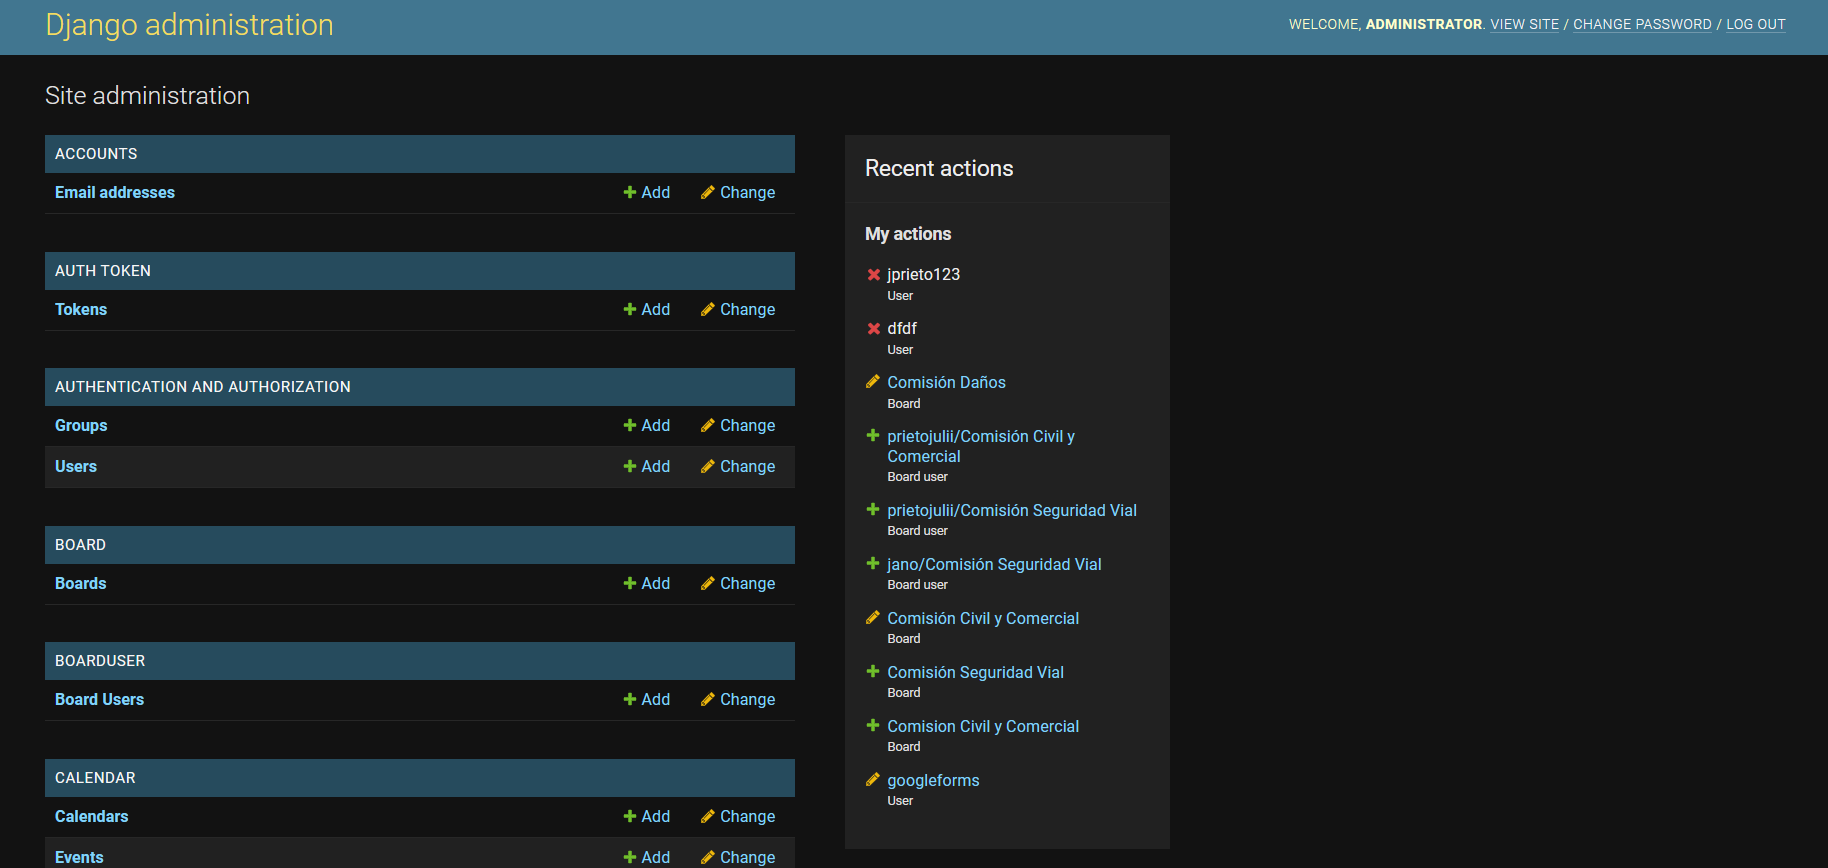
\includegraphics[width=1\linewidth]{fig/administracion.png}
    \caption{Interfaz de Administración de Django.}
    \label{fig:admin-interface}
\end{figure}

En esta interfaz, los administradores pueden realizar diversas acciones, como agregar, editar o eliminar registros, administrar permisos de usuario y conocer el estado del sistma.



\section{Tablero de Trabajo de Consultoría}
La página de consultoría es responsable de la administración de las consultas. Aquí, los tomadores de casos pueden revisar las consultas entrantes, representadas como tickets generados a través de formularios de Google. Pueden analizarlas y verificar si cumplen con las condiciones para ser patrocinadas por la entidad. Los tomadores de casos tienen la capacidad de crear, editar y eliminar consultas o enviarlas a una comisión para solicitar patrocinio.

La página está estructurada mediante paneles. El panel izquierdo contiene las consultas sin asignar, mientras que los paneles siguientes representan comisiones, cada uno con los tickets de las solicitudes de asignación. Para asignar una consulta a una comisión, basta con arrastrar la consulta al tablero de la comisión deseada. También es posible eliminar la solicitud volviendo a arrastrar el ticket al panel izquierdo. Para eliminar el ticket, simplemente posicione el mouse sobre el mismo, seleccione el menú que aparecerá y elija la opción "delete".

\begin{figure}[H]
    \centering
    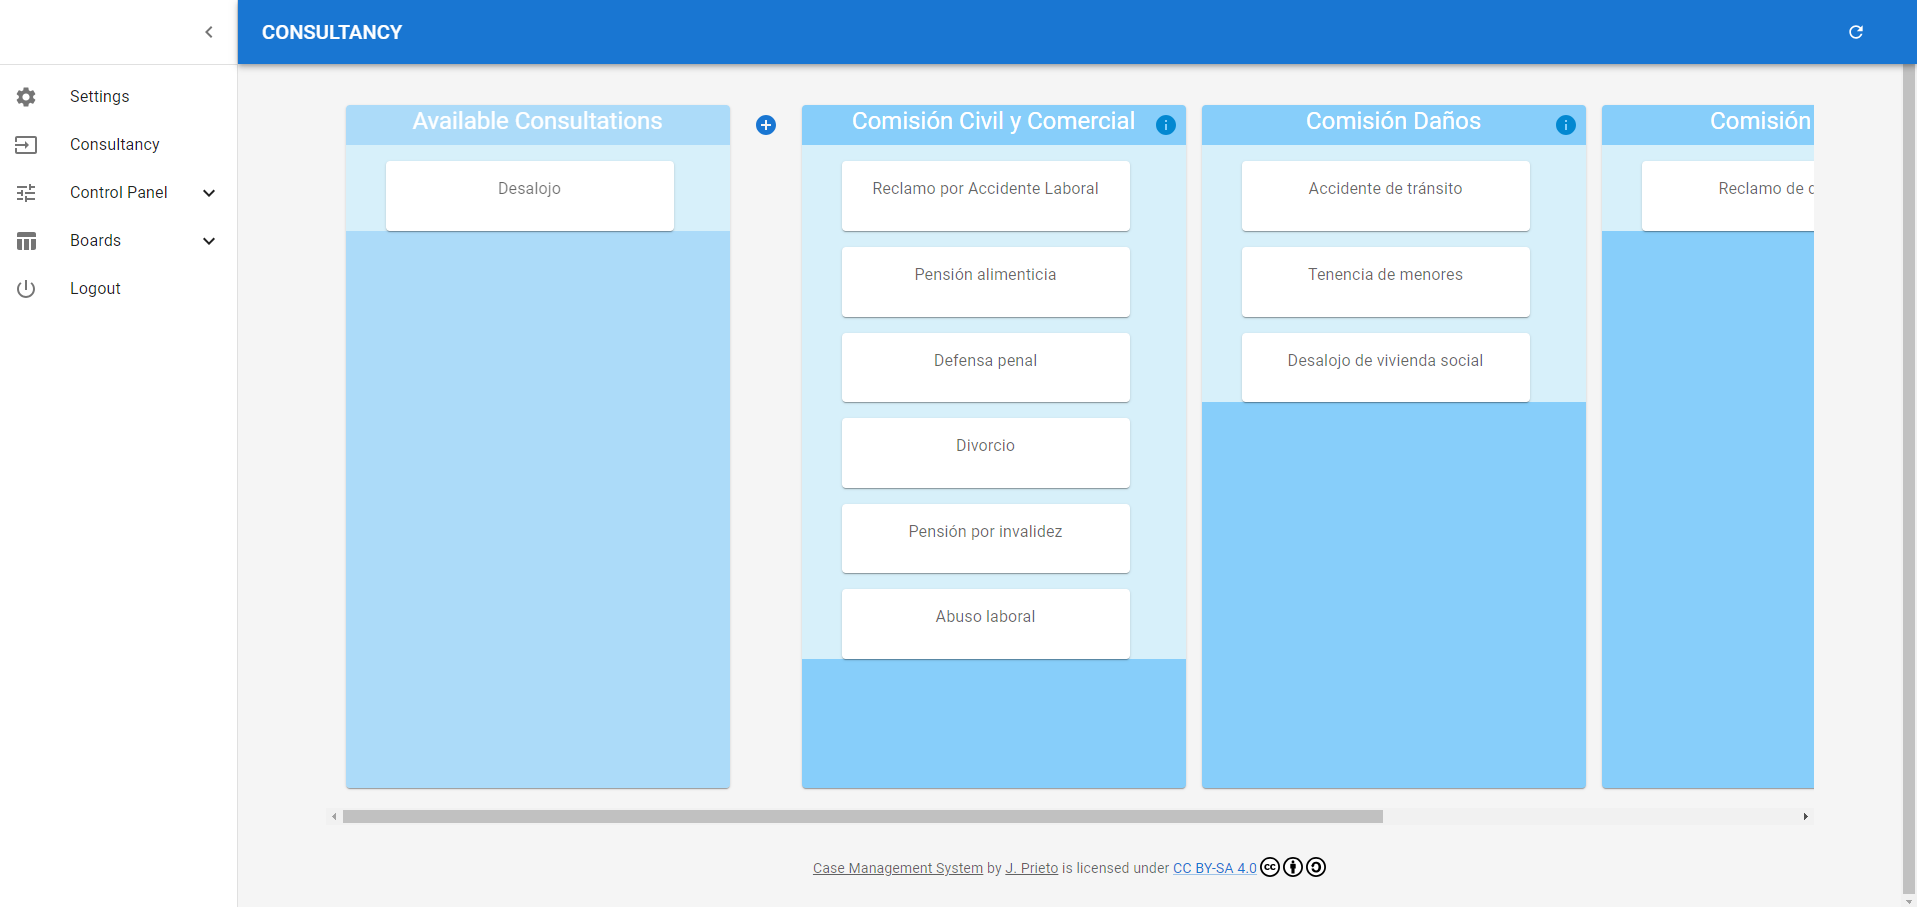
\includegraphics[width=1\linewidth]{fig/consultancy-real-page.png}
    \caption{Página de Consultoría}
    \label{fig:consultancy-real-page}
\end{figure}

Es importante mantener un registro del estado de cada comisión. Cada panel cuenta con un popper en el sector superior derecho que, al hacer clic, muestra la cantidad de consultas asignadas y la cantidad de consultas por estado (por hacer, en progreso o pausadas/bloqueadas). Además, incluye un historial de las asignaciones de los últimos 10 días, que muestra el ``tag'' de la consulta y la fecha de asignación.

\begin{figure}[H]
    \centering
    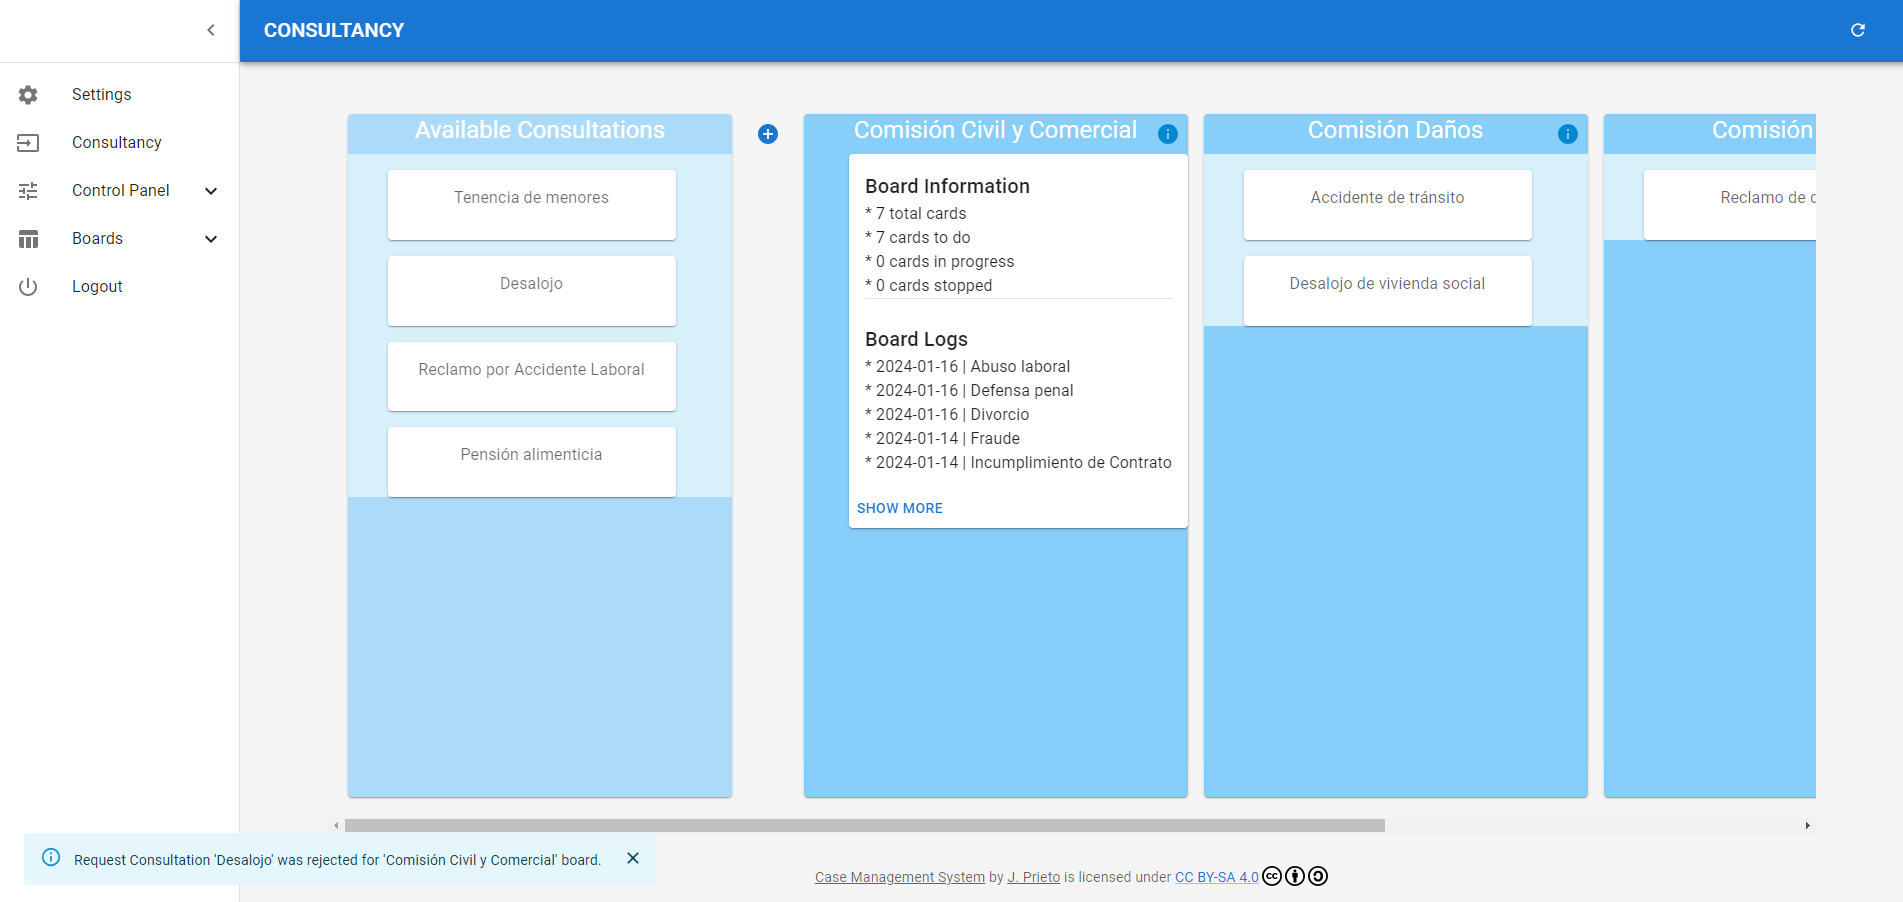
\includegraphics[width=1\linewidth]{fig/consultancy-real-page-logs-1.png}
    \caption{Historial de Asignaciones de una Comisión}
    \label{fig:consultancy-logs-1}
\end{figure}

Cuando la cantidad de consultas asignadas a la comisión en los últimos 10 días es extensa, aparecerá la opción ``show more'', que expandirá un panel con todas las asignaciones.

\begin{figure}[H]
    \centering
    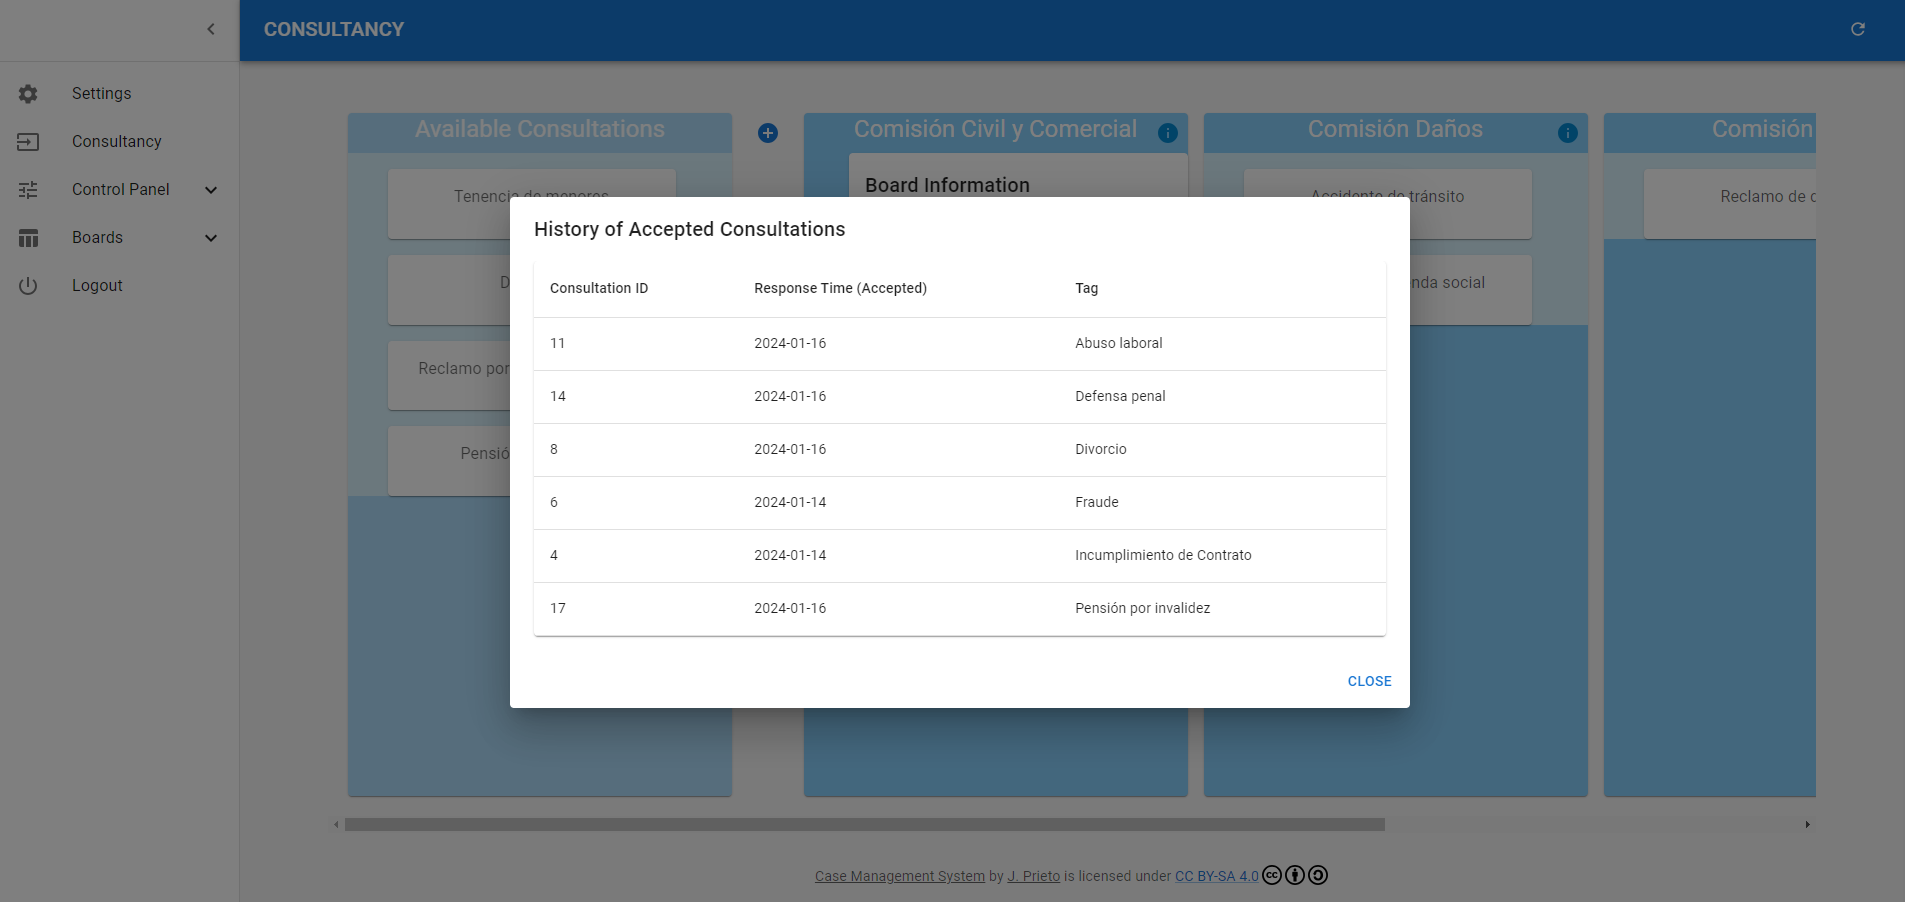
\includegraphics[width=1\linewidth]{fig/consultancy-real-page-logs-2.png}
    \caption{Panel Expandido de Historial de Asignaciones de una Comisión}
    \label{fig:consultancy-logs-2}
\end{figure}

El Usuario Tomador de Caso tiene la capacidad de crear consultas a través de la página de consultoría. Para hacerlo, se selecciona el botón con el símbolo ``+'' ubicado en el panel de entrada, y luego se completa el formulario según se muestra a continuación.

\begin{figure}[H]
    \centering
    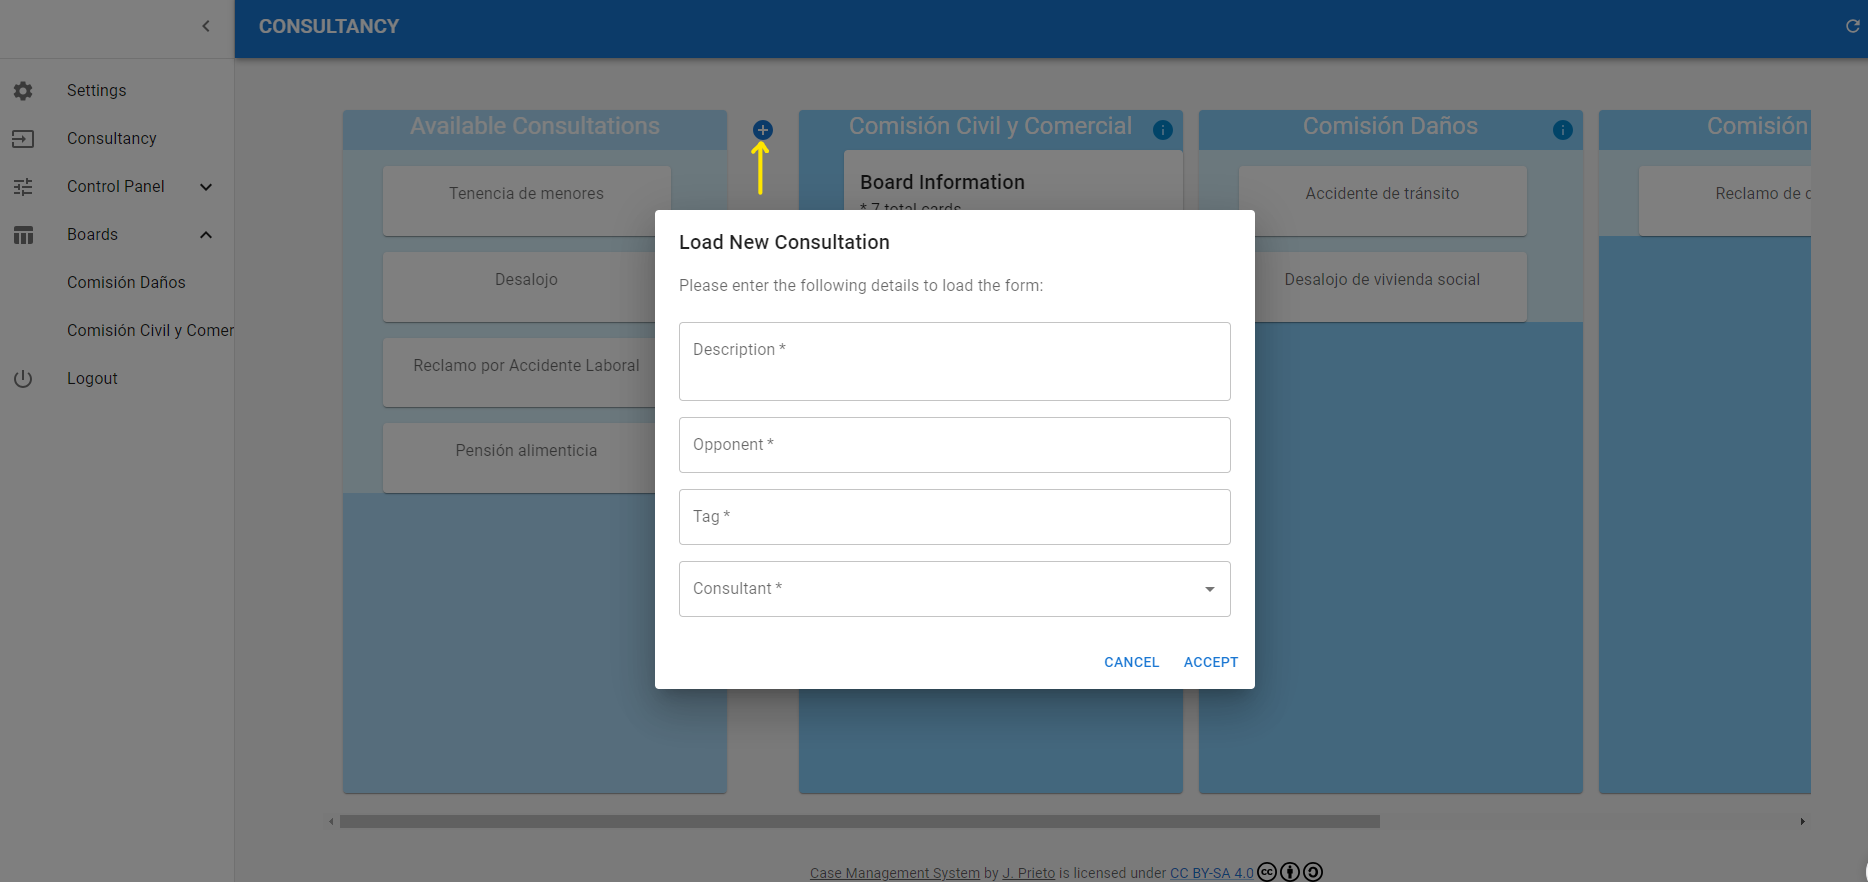
\includegraphics[width=1\linewidth]{fig/crear-consulta-consultancy.png}
    \caption{Formulario para Crear Consulta en la Página de Consultoría}
    \label{fig:formulario-crear-consulta}
\end{figure}




\section{Panel de Control}
El panel de control consta de dos pestañas principales: ``Consultations'' y ``Clients''. Ambas pestañas ofrecen tablas que pueden descargarse en formato PDF o CSV. Además, proporcionan opciones de filtro y permiten la edición, creación o eliminación de registros.

A continuación, se presenta la pestaña de ``Consultations'', que muestra una tabla con todas las consultas.

\begin{figure}[H]
    \centering
    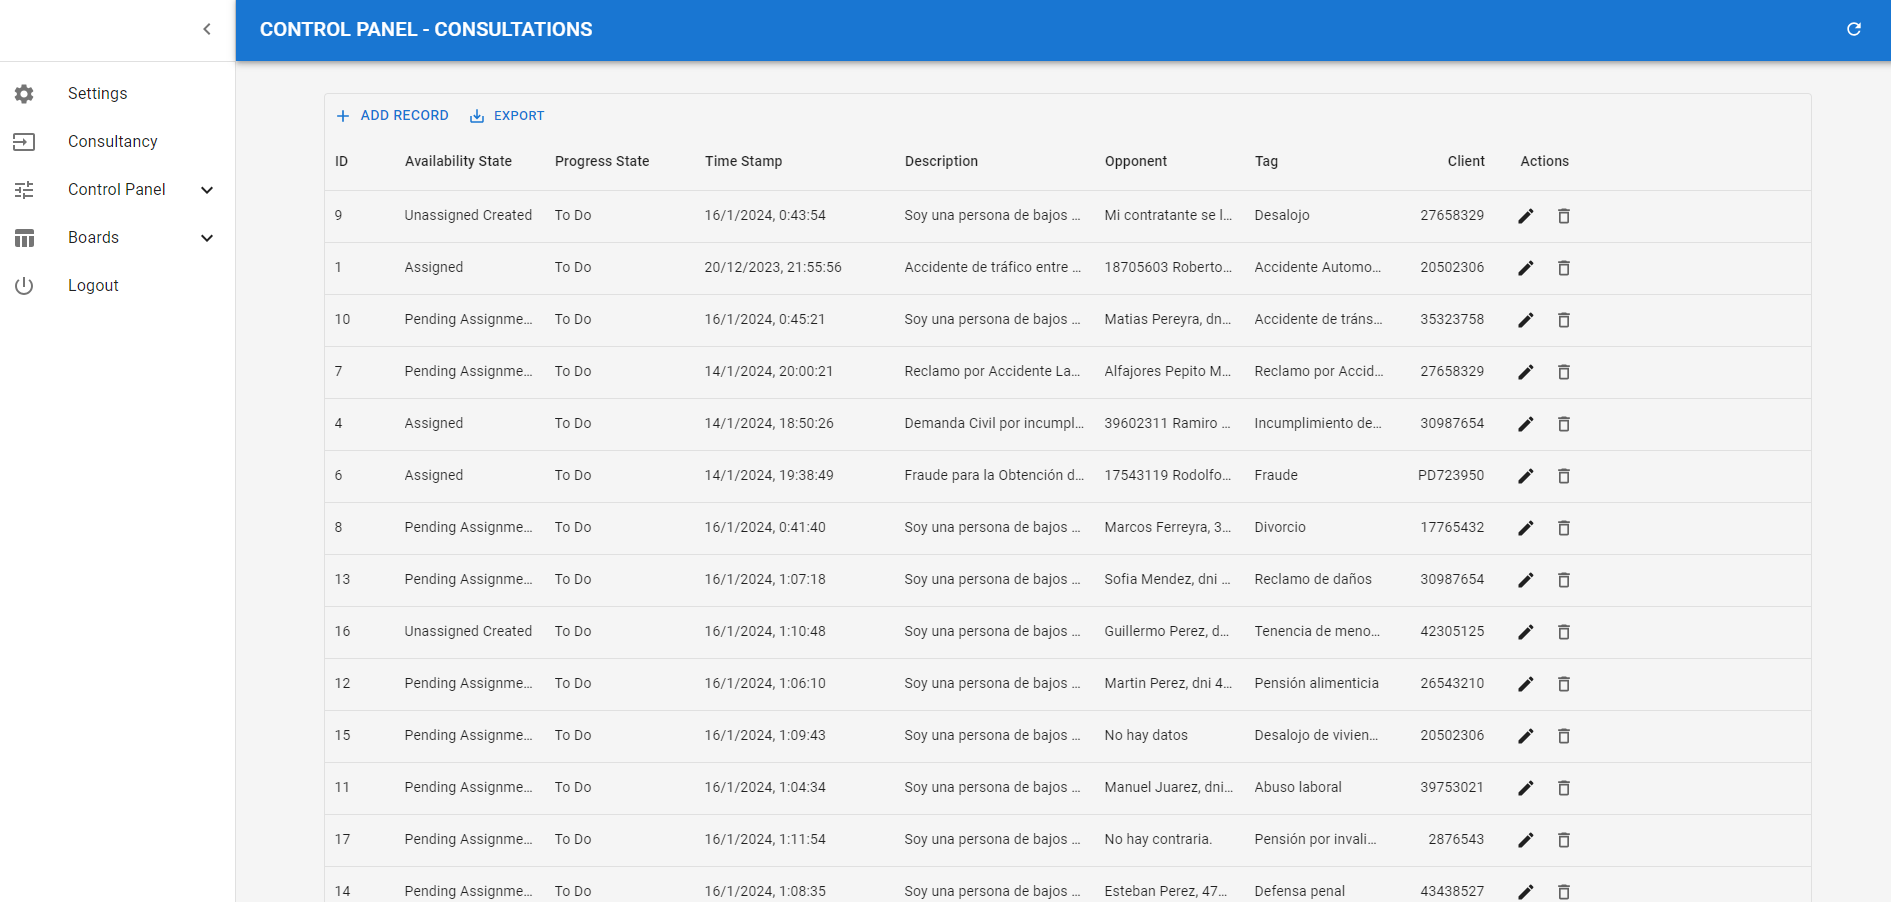
\includegraphics[width=1\linewidth]{fig/consultation-real-page.png}
    \caption{Tabla de Consultas en el Panel de Control.}
    \label{fig:consultations-table}
\end{figure}


A continuación, se presenta la pestaña de ``Clients'', que muestra una tabla con todos los clientes.

\begin{figure}[H]
    \centering
    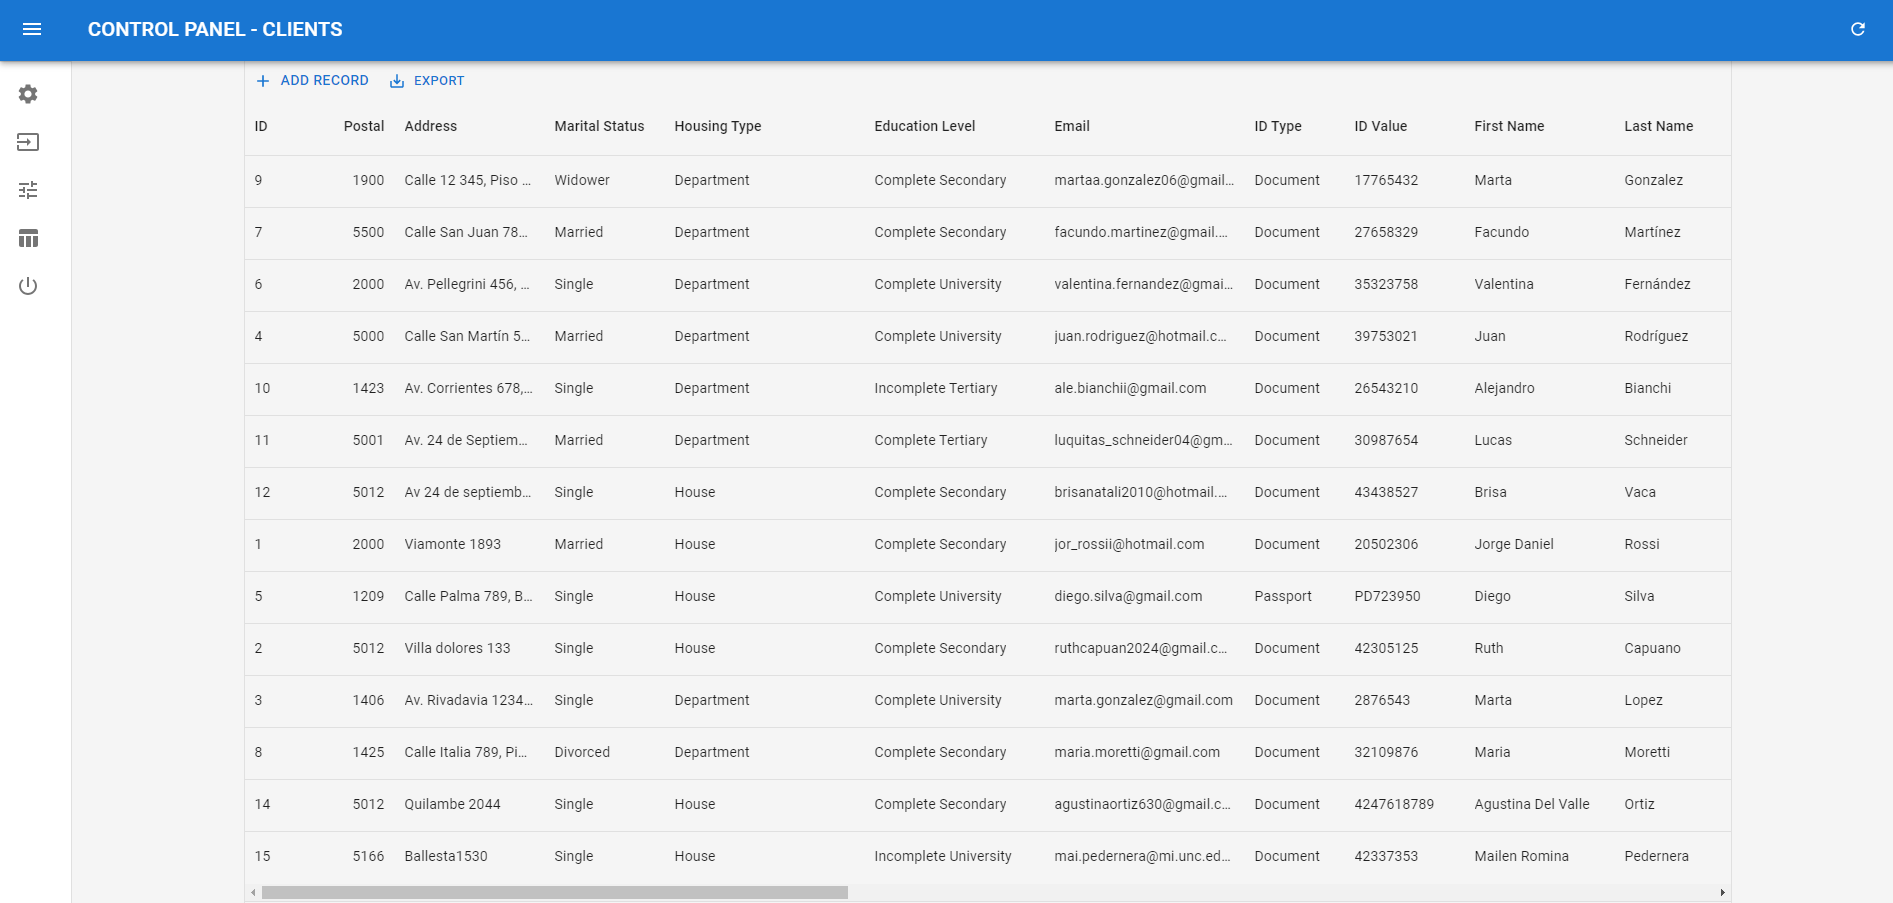
\includegraphics[width=1\linewidth]{fig/clients-real-page.png}
    \caption{Tabla de Clientes en el Panel de Control.}
    \label{fig:clients-table}
\end{figure}

Cada entrada en esta tabla puede ser eliminada o editada seleccionando los elementos en la última columna a la derecha de la entrada deseada. Además, es posible crear un nuevo registro haciendo clic en el botón ``Add Record'' en la parte superior.

La tabla también permite aplicar filtros a algunas de sus columnas. Para ello, cada columna tiene un tooltip que facilita la ordenación ascendente o descendente, filtrado y ocultamiento de la columna. A continuación, se muestra un ejemplo de aplicación de un filtro a la columna ``progress state'' de la tabla ``consultations''.

\begin{figure}[H]
    \centering
    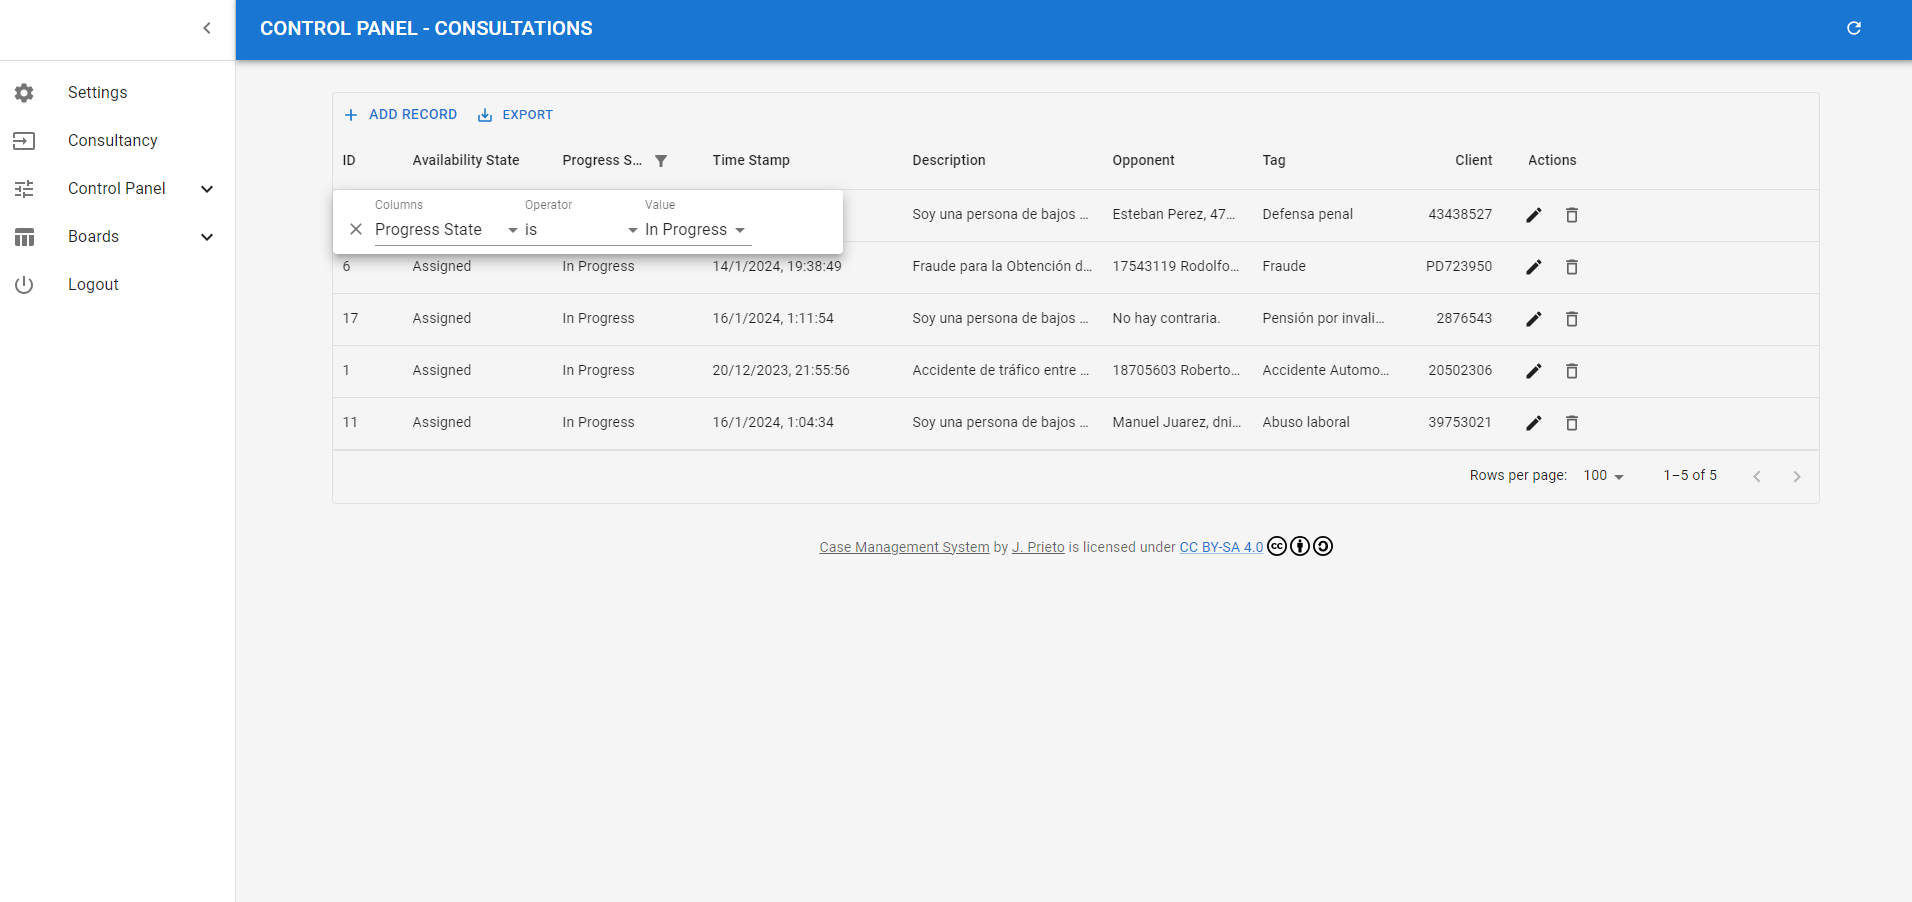
\includegraphics[width=1\linewidth]{fig/tabla-filter.png}
    \caption{Aplicación de un Filtro en la Columna Progress State}
    \label{fig:tabla-filtro-ejemplo}
\end{figure}



\section{Tablero de Trabajo para la Comisión}
Cada comisión cuenta con un ``Board'', el cual los usuarios con acceso podrán visualizar desde la sección ``Boards'' en el menú desplegable de la página.

Este espacio está organizado en paneles, siendo el primero a la izquierda el panel de entrada de solicitudes de asignación de casos. Para aceptar una solicitud, basta con arrastrar el ticket de la consulta a alguno de los paneles internos del board. Para rechazarla, se puede seleccionar la opción ``rejected'' desde el menú del ticket, el cual se hace visible acercando el ratón sobre él.

Los paneles a la izquierda son flexibles y pueden ser creados según la necesidad del usuario, ya sea como organizadores, separadores de consultas, o para cualquier otro agrupamiento conveniente. Por ejemplo, podrían ser utilizados un panel por profesor, otro por estado de progreso de las consultas, o cualquier otro criterio de agrupación preferido.

\begin{figure}[H]
    \centering
    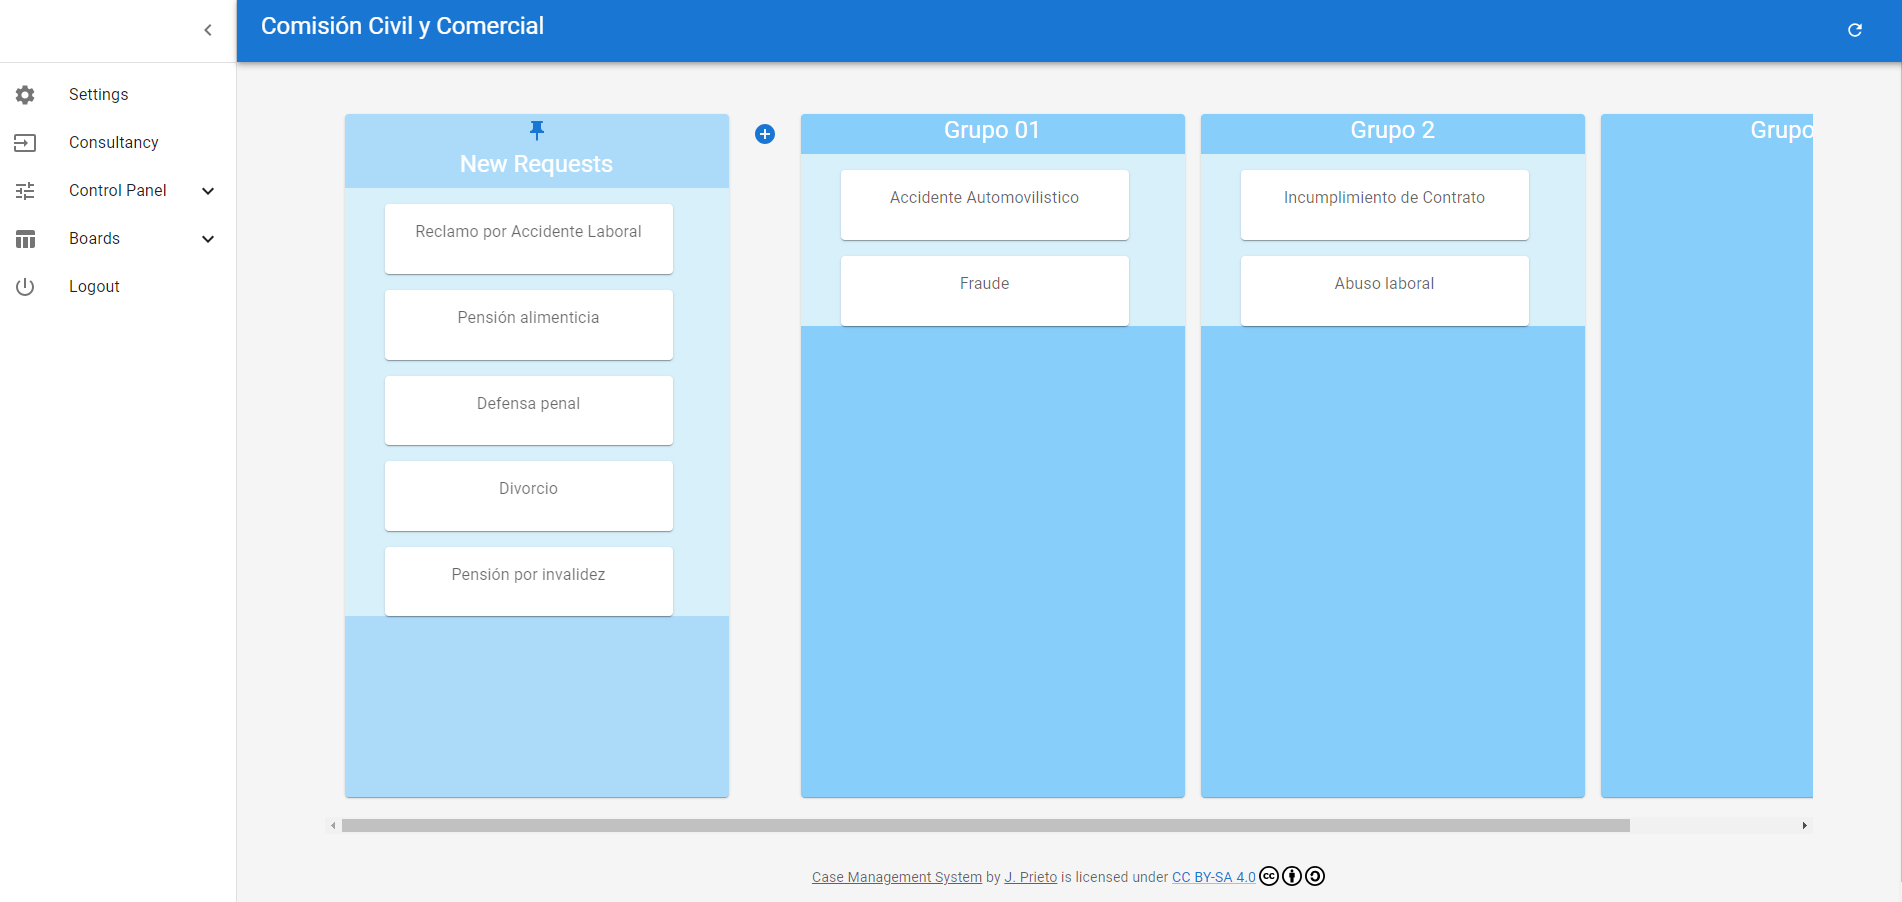
\includegraphics[width=1\linewidth]{fig/board-real-page.png}
    \caption{Página Board de la Comisión}
    \label{fig:board-real-page}
\end{figure}

Cada panel se puede crear utilizando el botón ``+'' e ingresando el nombre correspondiente. Asimismo, se pueden eliminar a través del menú del panel o editar el título haciendo doble clic sobre él (siempre y cuando no existan tickets en el tablero). Además, el board puede ser renombrado haciendo doble clic sobre el título.

\begin{figure}[H]
    \centering
    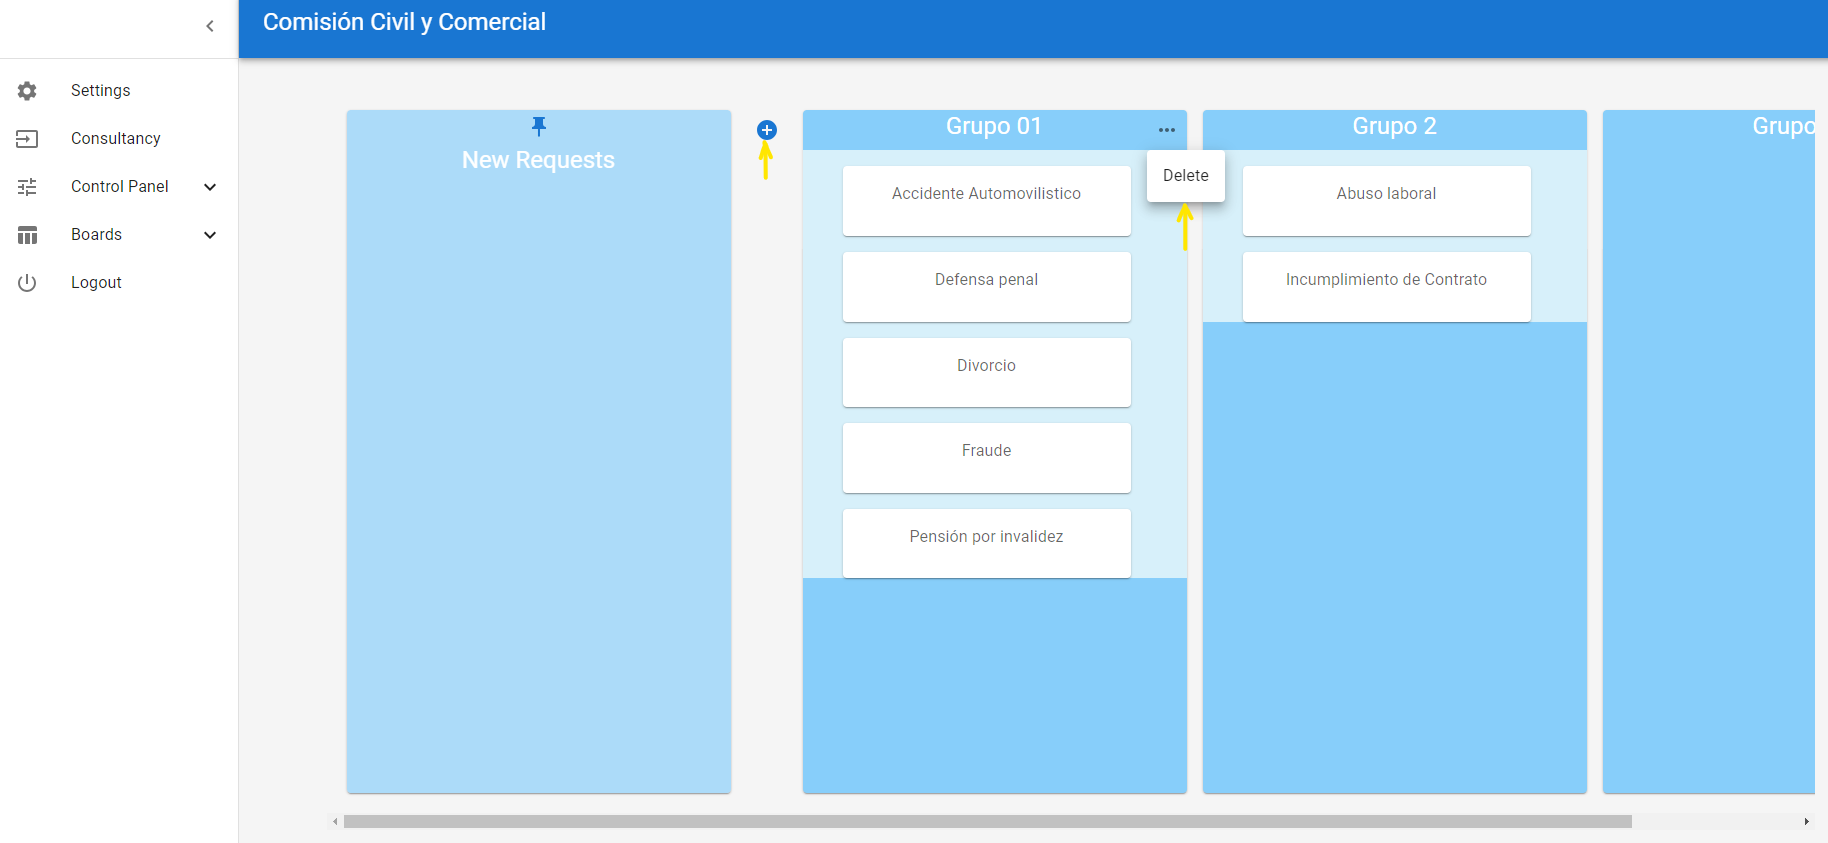
\includegraphics[width=1\linewidth]{fig/delete-panel.png}
    \caption{Botones para eliminar o crear un Panel del Board}
    \label{fig:delete-panel}
\end{figure}





\section{Detalles de la Consulta}\label{sec:info-consulta}

Para obtener más detalles sobre una consulta específica, se debe hacer click en la tarjeta correspondiente, lo que desplegará un cuadro con tres pestañas distintas.

\begin{figure}[H]
    \centering
    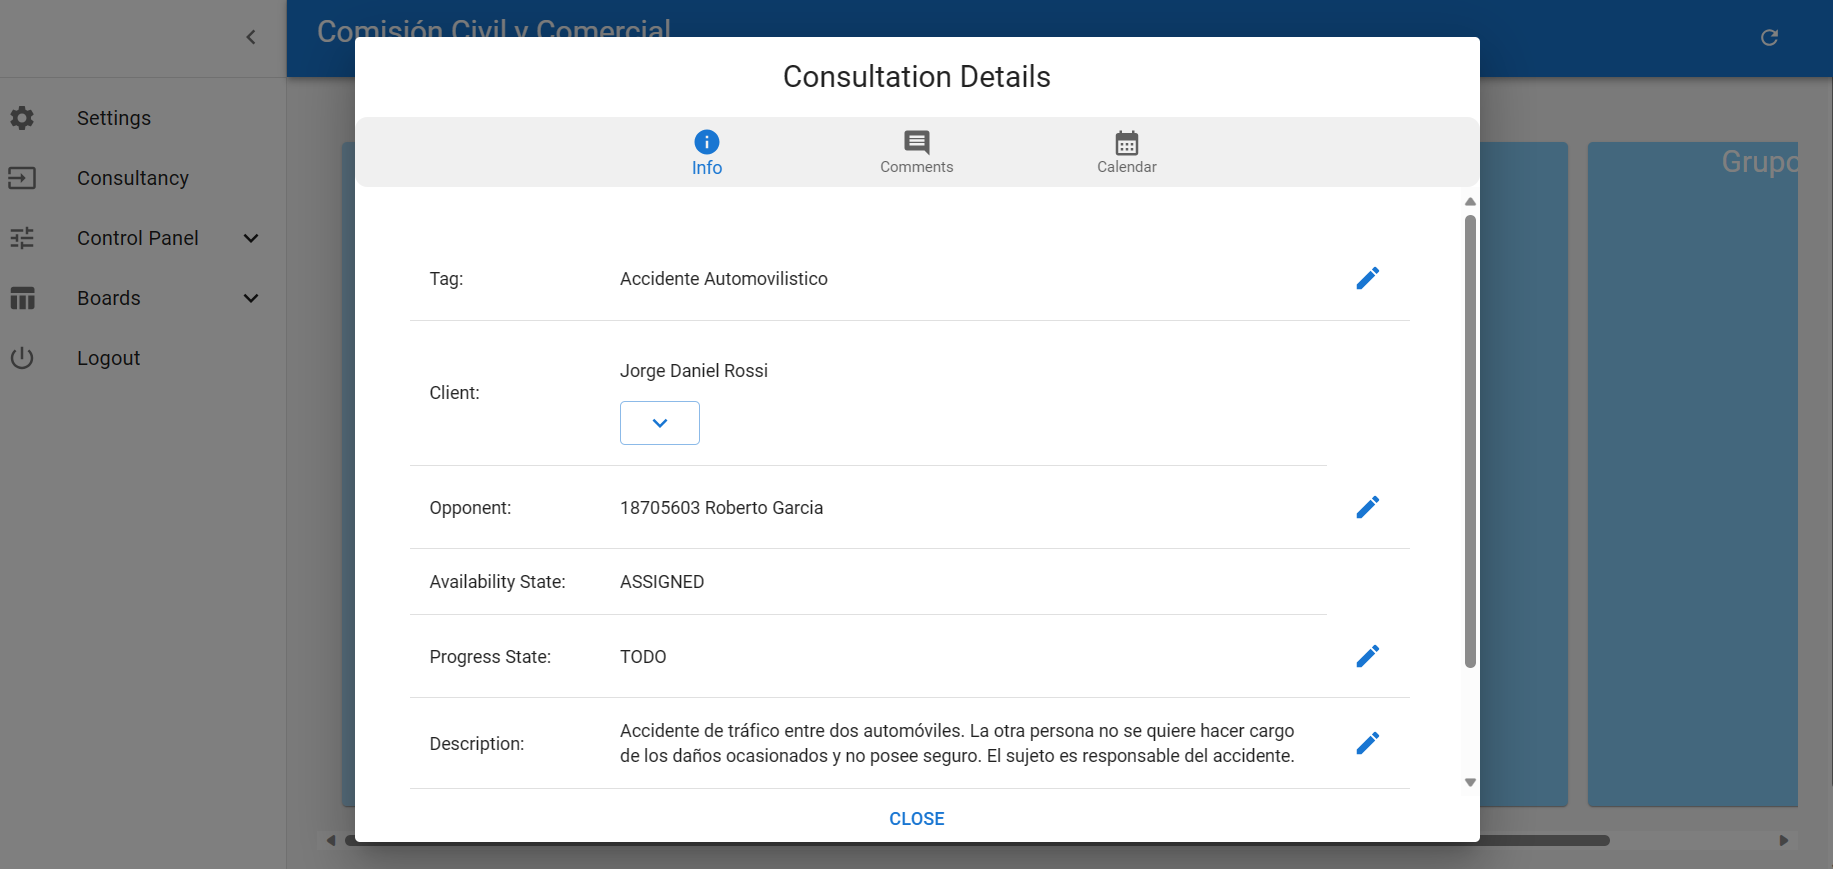
\includegraphics[width=1\linewidth]{fig/info-consulta.png}
    \caption{Ventana de Información de Consulta.}
    \label{fig:consulta-info}
\end{figure}

La primera pestaña presenta información organizada sobre el cliente y los detalles de la consulta.

\begin{figure}[H]
    \centering
    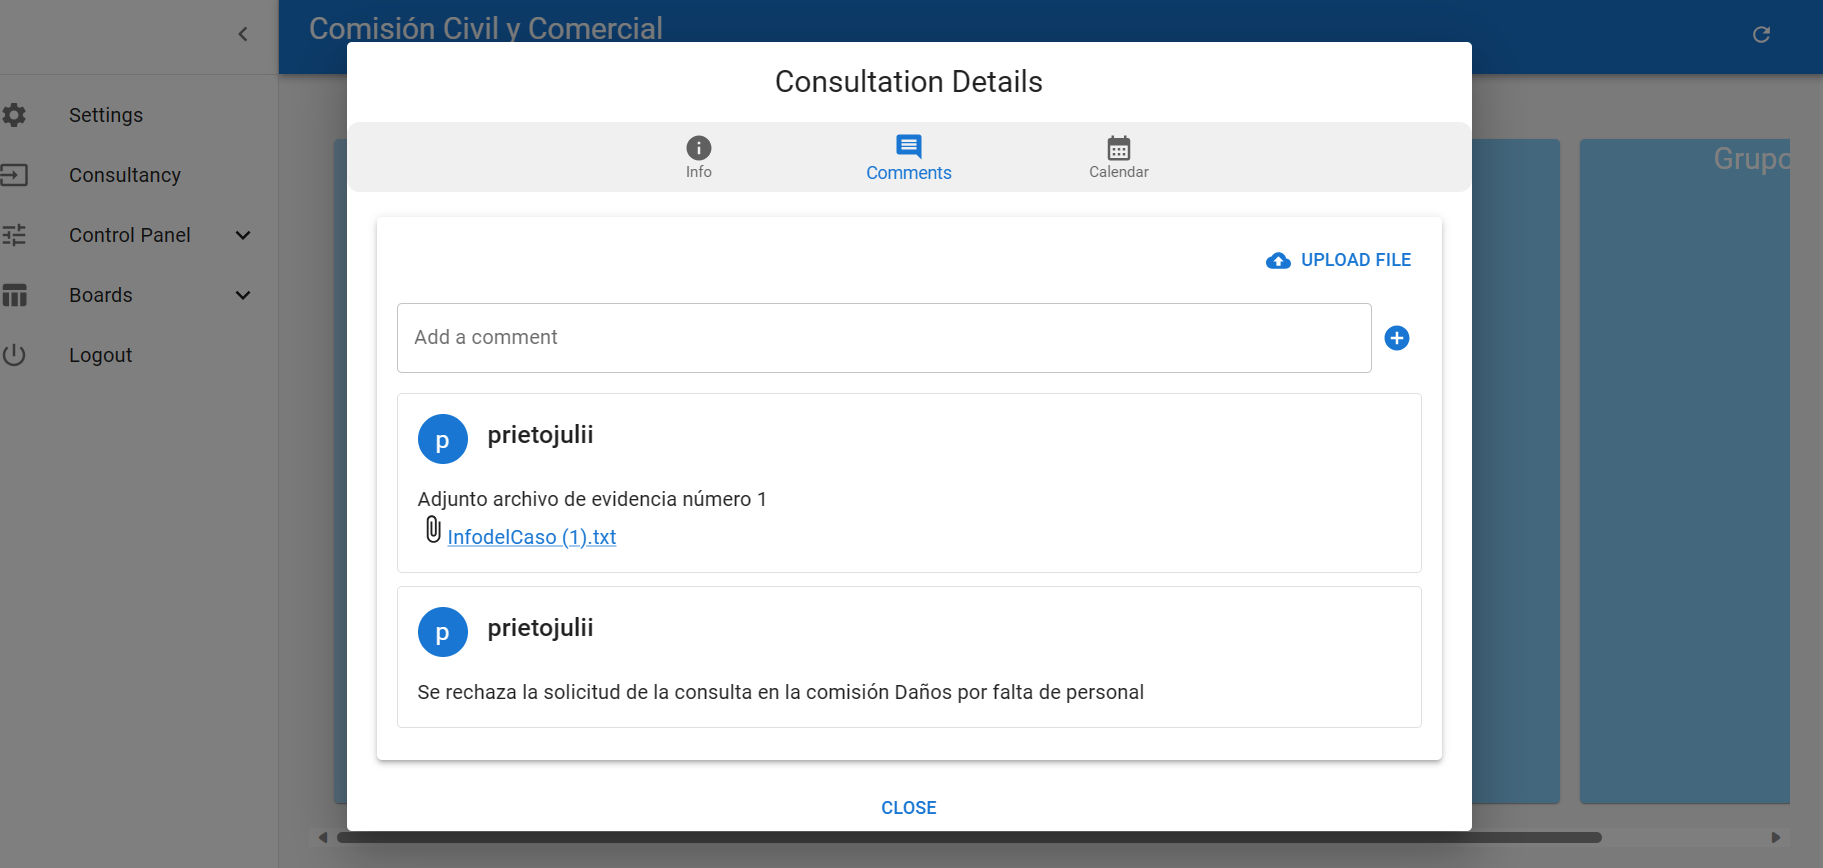
\includegraphics[width=1\linewidth]{fig/comentario-consulta.png}
    \caption{Sección de Comentarios y Archivos.}
    \label{fig:consulta-comentarios}
\end{figure}

La segunda pestaña es una sección dedicada para registrar comentarios y archivos relevantes que contribuyan al seguimiento del caso.

\begin{figure}[H]
    \centering
    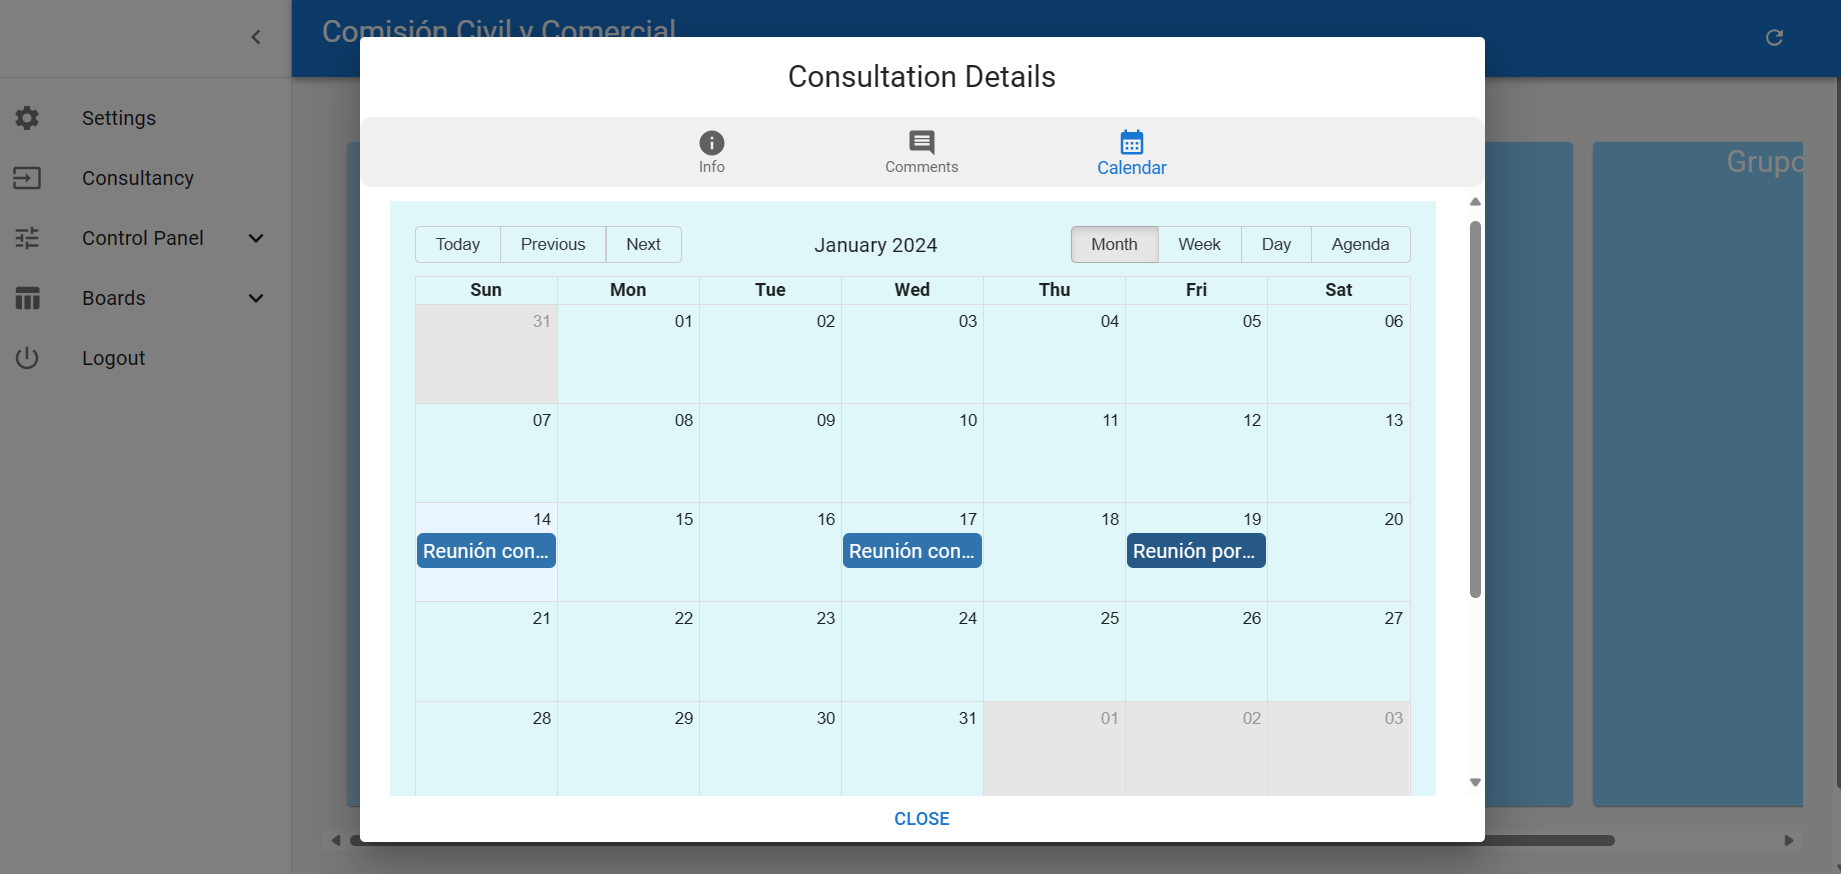
\includegraphics[width=1\linewidth]{fig/consulta-calendar-1.png}
    \caption{Calendario de Consulta.}
    \label{fig:consulta-calendar-1}
\end{figure}

La tercera ventana es un calendario que permite registrar eventos relacionados con el caso, como reuniones o fechas importantes.

\begin{figure}[H]
    \centering
    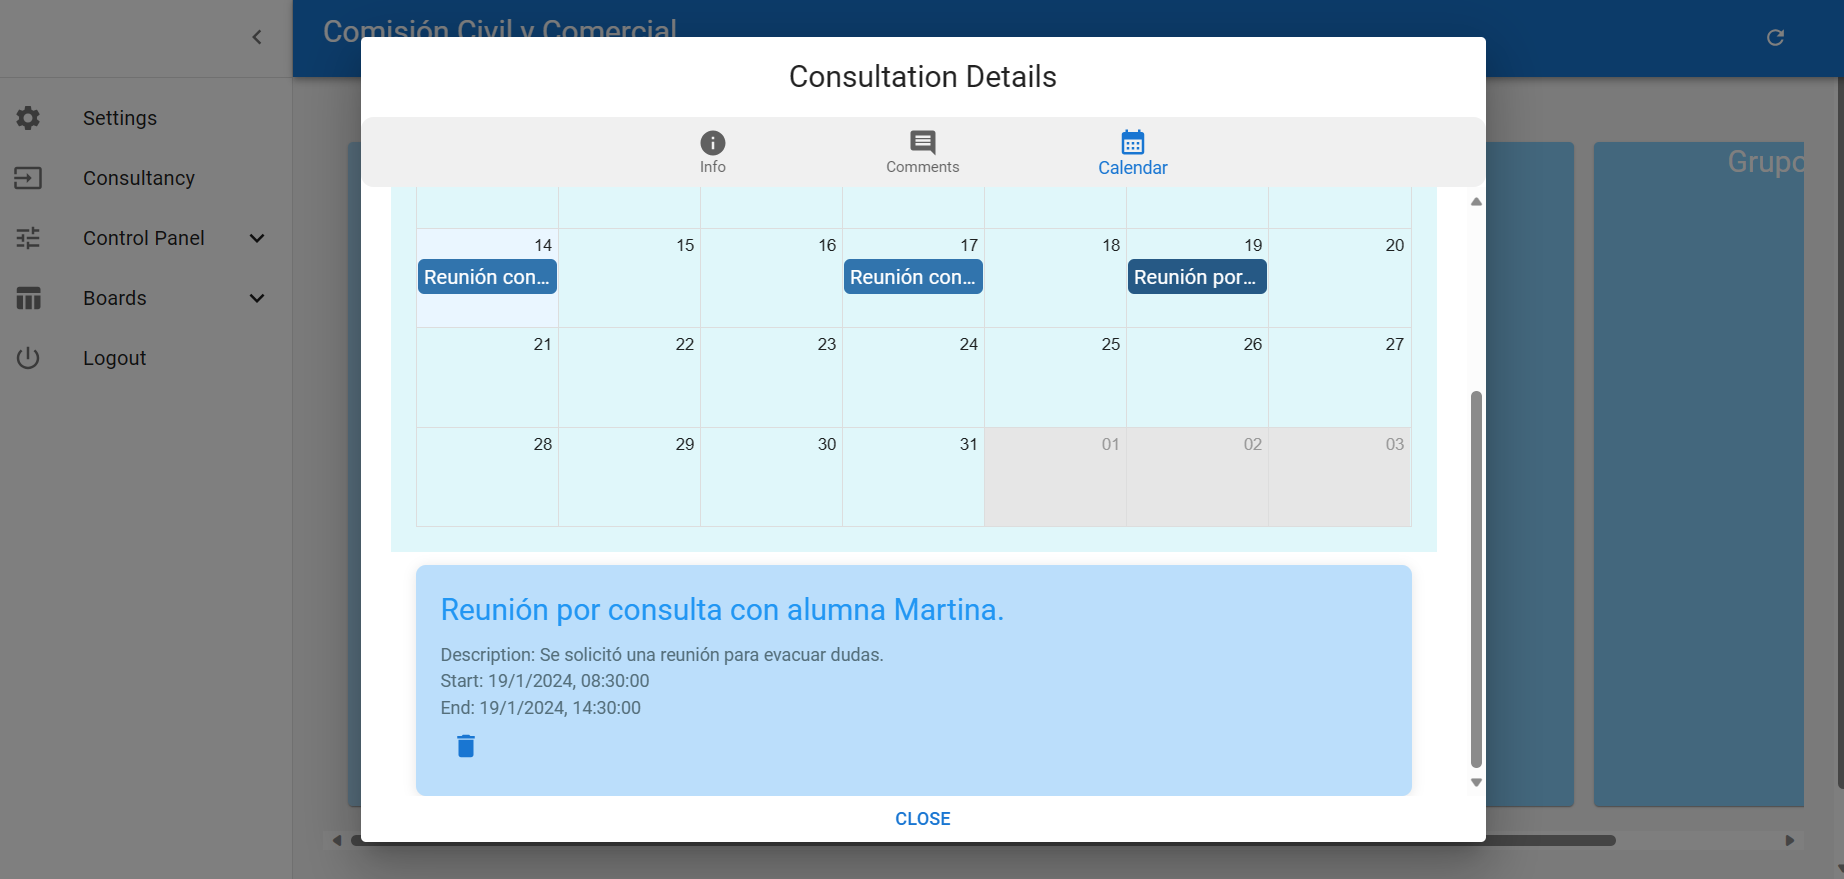
\includegraphics[width=1\linewidth]{fig/consulta-calendar-2.png}
    \caption{Detalle de Evento del Calendario de Consulta.}
    \label{fig:consulta-calendar-2}
\end{figure}
Al seleccionar un evento en el calendario, se desplegará una vista detallada con información adicional.

\begin{figure}[H]
    \centering
    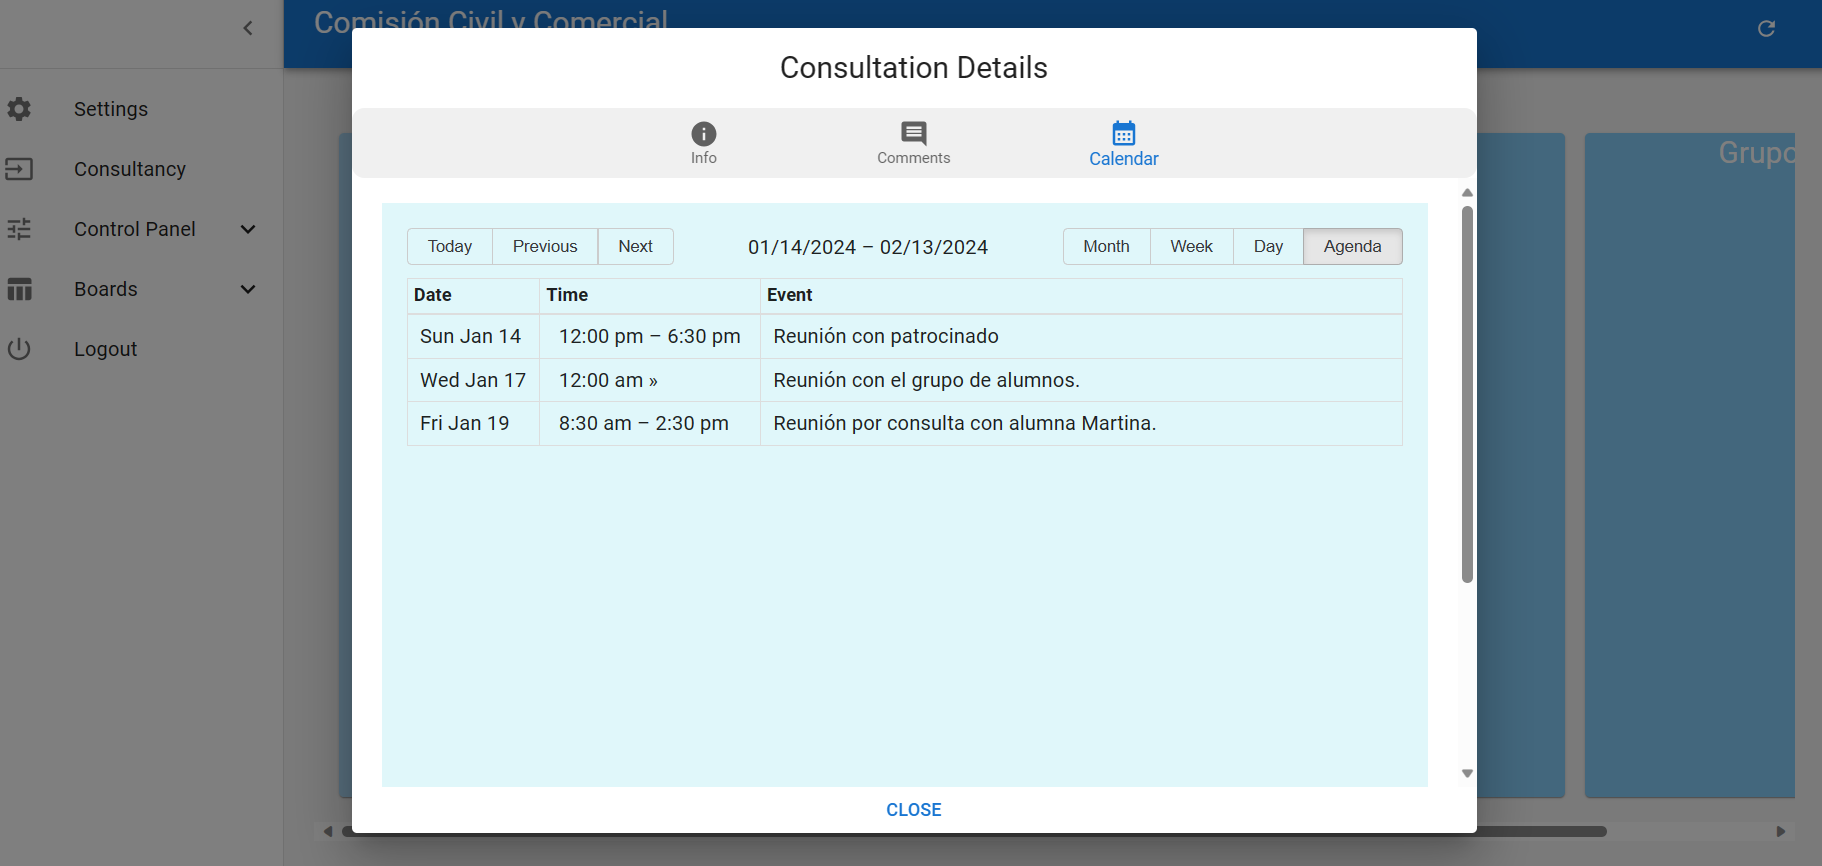
\includegraphics[width=1\linewidth]{fig/consulta-calendar-3.png}
    \caption{Vista Agenda de Calendario de Consulta.}
    \label{fig:consulta-calendar-3}
\end{figure}

Este calendario ofrece varias vistas, como mensual, semanal, diaria o en formato de agenda, según se visualiza en la imagen anterior. Es una herramienta clave para organizar y dar seguimiento a eventos relevantes asociados a la consulta.

\section{Configuración de Cuenta}\label{sec:configuracion-cuenta}

La sección de configuración de cuenta, accesible desde la página de ``Settings'', proporciona la capacidad de visualizar y editar información personalizada, como el nombre de usuario y la contraseña.

\begin{figure}[H]
    \centering
    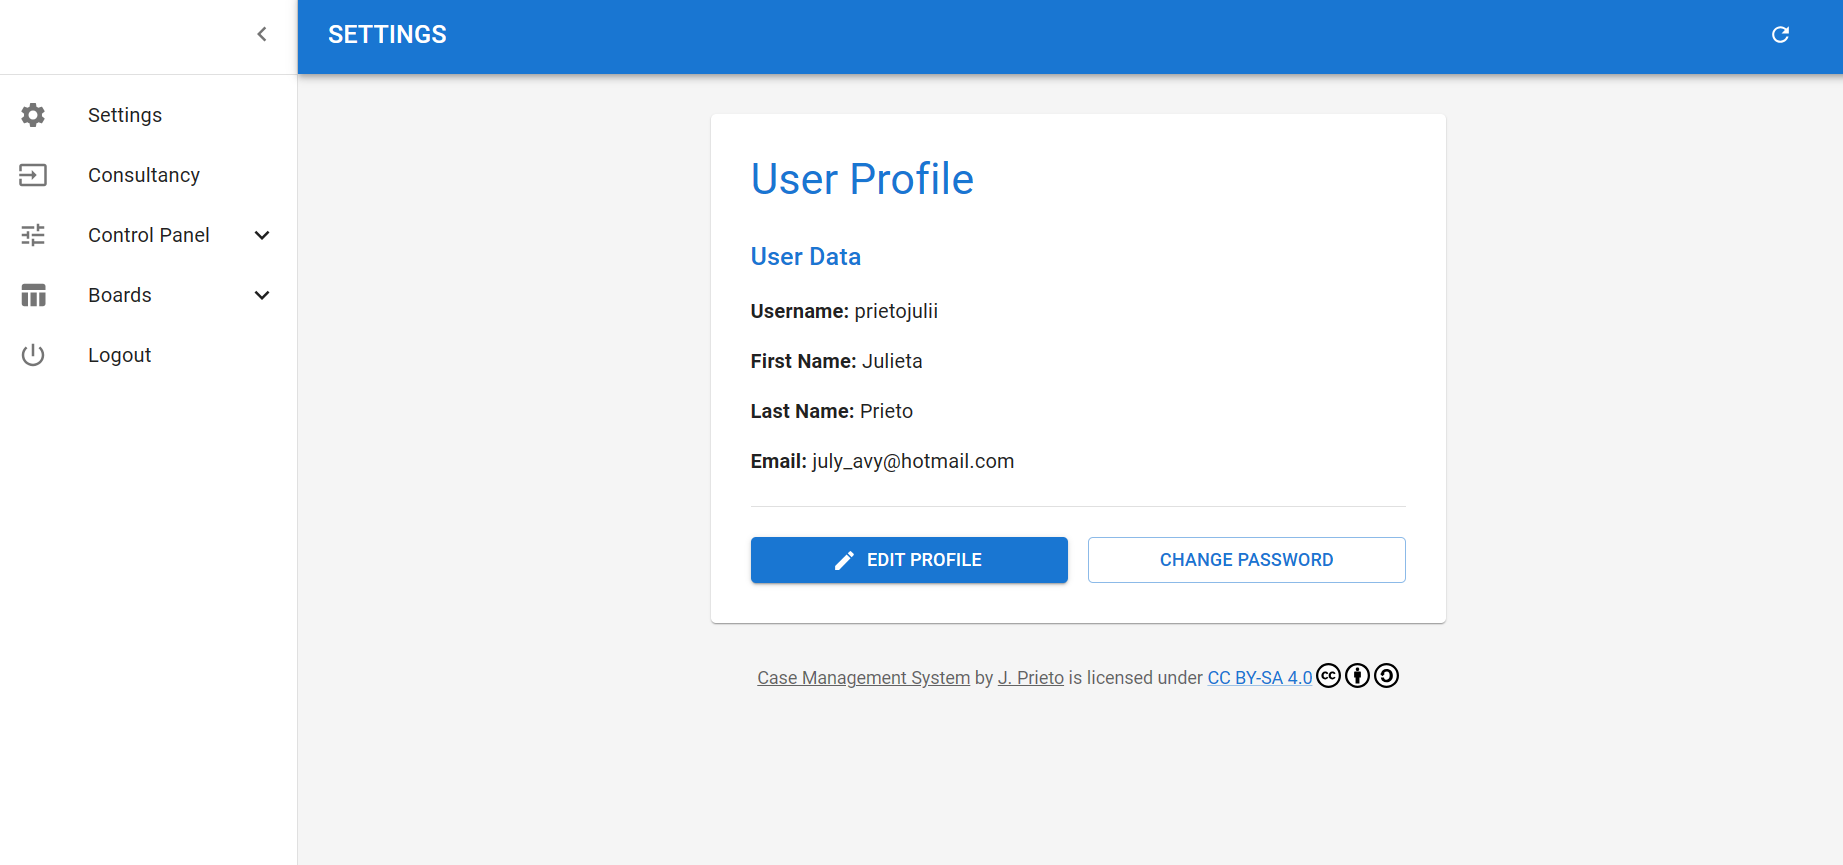
\includegraphics[width=1\linewidth]{fig/settings-real-page.png}
    \caption{Página de Configuración de Cuenta.}
    \label{fig:settings-page}
\end{figure}

    \input{sections/06_Implementación_Test}
    \appendix
    \chapter{Configuración de Nginx}\label{cap:apendix-nginx}
% Configuración de estilo para el código
\lstset{
    language=sh,
    backgroundcolor=\color{white},
    basicstyle=\footnotesize\ttfamily,
    keywordstyle=\color{blue},
    commentstyle=\color{green},
    stringstyle=\color{red},
    captionpos=b,
    breaklines=true,
    showstringspaces=false,
    numbers=left,
    numberstyle=\tiny,
    frame=single,
    rulecolor=\color{black}
}

\section{Configuración del Ngnix como Reverse Proxy}\label{subsec:nginx_explicacion}
El archivo de configuración Nginx utilizado como proxy reverse en el Stack de contenedores es el siguiente:
\begin{lstlisting}[caption={Configuración de Nginx Reverse Proxy}, label={cod:nginx}, captionpos=b]
limit_conn_zone $binary_remote_addr zone=addr:10m;

upstream gunicorn{
    server appserver:8000;
}

upstream daphne{
    server appserver:8001;
}

upstream frontend{
    server frontend:3000;
}

server {
    client_body_timeout 5s;
    client_header_timeout 5s; # Closing Slow Connections
    server_tokens off;
    listen 80;
    listen  [::]:80;
    server_name  proyecto-patrocinio.fcefyn.unc.edu.ar;

    location / {
        limit_req zone=mylimit burst=20 nodelay;
        limit_conn addr 10;
        try_files $uri @proxy_frontend;
    }
    location /api {
        limit_req zone=mylimit burst=20 nodelay;
        limit_conn addr 10;
        try_files $uri @proxy_api_wsgi;
    }
    location /ws {
        limit_req zone=mylimit burst=20 nodelay;
        limit_conn addr 10;
        try_files $uri @proxy_api_asgi;
    }
    location /admin {
        limit_req zone=mylimit burst=20 nodelay;
        limit_conn addr 10;
        root /usr/src/app/django_static;
        include /etc/nginx/mime.types;
        try_files $uri @proxy_api_wsgi;
    }

    # redirect to django app: React server
    location @proxy_frontend {
        proxy_pass http://frontend;
        proxy_redirect off;
        proxy_cache_bypass  $http_upgrade;
        proxy_set_header Upgrade           $http_upgrade;
        proxy_set_header Connection        "upgrade";
        proxy_set_header Host              $host;
        proxy_set_header X-Real-IP         $remote_addr;
        proxy_set_header X-Forwarded-For   $proxy_add_x_forwarded_for;
        proxy_set_header X-Forwarded-Proto $scheme;
        proxy_set_header X-Forwarded-Host  $host;
        proxy_set_header X-Forwarded-Port  $server_port;
        proxy_set_header Cookie $http_cookie;
    }

    # redirect to django app: API REST
    location @proxy_api_wsgi {
        proxy_pass http://gunicorn;
        proxy_redirect off;
        proxy_cache_bypass  $http_upgrade;
        proxy_set_header Upgrade           $http_upgrade;
        proxy_set_header Connection        "upgrade";
        proxy_set_header Host              $host;
        proxy_set_header X-Real-IP         $remote_addr;
        proxy_set_header X-Forwarded-For   $proxy_add_x_forwarded_for;
        proxy_set_header X-Forwarded-Proto $scheme;
        proxy_set_header X-Forwarded-Host  $host;
        proxy_set_header X-Forwarded-Port  $server_port;
        proxy_set_header Cookie $http_cookie;
    }

    # redirect to django app with WebSocket
    location @proxy_api_asgi {
        proxy_pass http://daphne;
        proxy_redirect off;
        proxy_cache_bypass  $http_upgrade;
        proxy_set_header Upgrade           $http_upgrade;
        proxy_set_header Connection        "upgrade";
        proxy_set_header Host              $host;
        proxy_set_header X-Real-IP         $remote_addr;
        proxy_set_header X-Forwarded-For   $proxy_add_x_forwarded_for;
        proxy_set_header X-Forwarded-Proto $scheme;
        proxy_set_header X-Forwarded-Host  $host;
        proxy_set_header X-Forwarded-Port  $server_port;
        proxy_set_header Cookie $http_cookie;
    }

    location /django_static/ {
        limit_req zone=mylimit burst=20 nodelay;
        limit_conn addr 10;
        autoindex on;
        alias /usr/share/nginx/staticfiles/cms/django/;
    }
}
\end{lstlisting}







\section{Configuración del Ngnix como Servidor}

Por otro lado, el servidor contaba con un Servidor Nginx instalado y en funcionamiento sirviendo otras aplicaciones.
Para agregar el servicio Case Managment System se agregó el siguiente archivo en el directorio \textbf{etc/nginx/conf.d/proyecto-patrocinio.fcefyn.unc.edu.ar.conf}:



\begin{lstlisting}[caption={Configuración de Nginx en el Servidor}, label={cod:nginx}, captionpos=b]

server {
    server_name proyecto-patrocinio.fcefyn.unc.edu.ar;

    location / {
        proxy_pass http://localhost:8081;
        proxy_redirect off;
        proxy_cache_bypass  $http_upgrade;
        proxy_set_header Upgrade           $http_upgrade;
        proxy_set_header Connection        "upgrade";
        proxy_set_header Host              $host;
        proxy_set_header X-Real-IP         $remote_addr;
        proxy_set_header X-Forwarded-For   $proxy_add_x_forwarded_for;
        proxy_set_header X-Forwarded-Proto $scheme;
        proxy_set_header X-Forwarded-Host  $host;
        proxy_set_header X-Forwarded-Port  $server_port;
        proxy_set_header Cookie $http_cookie;
    }

    listen 443 ssl; # managed by Certbot
    ssl_certificate /etc/letsencrypt/live/proyecto-patrocinio.fcefyn.unc.edu.ar/fullchain.pem; # managed by Certbot
    ssl_certificate_key /etc/letsencrypt/live/proyecto-patrocinio.fcefyn.unc.edu.ar/privkey.pem; # managed by Certbot
    include /etc/letsencrypt/options-ssl-nginx.conf; # managed by Certbot
    ssl_dhparam /etc/letsencrypt/ssl-dhparams.pem; # managed by Certbot

}

server {
    if ($host = proyecto-patrocinio.fcefyn.unc.edu.ar) {
        return 301 https://$host$request_uri;
    } # managed by Certbot


    listen 80;
    server_name proyecto-patrocinio.fcefyn.unc.edu.ar;
    return 404; # managed by Certbot


}
\end{lstlisting}
    \chapter{Endpoints de Formularios}\label{cap:anexo-expoint-forms}

\section{Endpoint del Formulario Registro de Cliente}

\subsection*{URL}
\texttt{http://\{\{ip\}\}:\{\{port\}\}/api/clients/client/form/}

\subsection*{Método}
POST

\subsection*{Body de Ejemplo:}
A continuación se presenta un ejemplo.
\begin{lstlisting}[caption=Body de Ejemplo, label=example-body]
{
    "first_name": "Martina",
    "last_name": "Gutierrez",
    "id_type": "DOCUMENT",
    "id_value": "42304328",
    "birth_date": "2000-11-13",
    "sex": "FEMALE",
    "marital_status": "SINGLE",
    "studies": "INCOMPLETE_UNIVERSITY",
    "email": "martina2000@gmail.com",
    "housing_type": "HOUSE",
    "locality": 9,
    "address": "Av. Patria 1234",
    "postal": "5000",
    "employment": "programmer",
    "salary": "123",
    "other_income": "No tengo otros ingresos",
    "amount_other_income": "0",
    "amount_retirement": "0",
    "amount_pension": "0",
    "vehicle": "No tengo otros vehiculos",
    "tel": [
        "3512254210",
        "+54 9 25578784"
    ],
    "partner_salary": "0"
}
\end{lstlisting}
\subsection*{Campos del Body:}

\begin{table}[H]
    \centering
    \begin{tabular}{|l|l|p{5cm}|p{5cm}|}
        \hline
        \textbf{Campo} & \textbf{Tipo} & \textbf{Opciones} & \textbf{Descripción} \\ \hline
        first\_name & String & & Nombre del consultante. \\ \hline
        last\_name & String & & Apellido del consultante. \\ \hline
        id\_type & String & DOCUMENT, PASSPORT & Tipo de documento de identidad. \\ \hline
        id\_value & String & & Valor del documento de identidad. \\ \hline
        birth\_date & String & & Fecha de nacimiento del consultante. \\ \hline
        sex & String & MALE, FEMALE & Género del consultante. \\ \hline
        marital\_status & String & SINGLE, MARRIED, DIVORCED, WIDOWER & Estado civil del consultante. \\ \hline
        studies & String & INCOMPLETE\_PRIMARY, COMPLETE\_PRIMARY, INCOMPLETE\_SECONDARY, COMPLETE\_SECONDARY, INCOMPLETE\_TERTIARY, COMPLETE\_TERTIARY, INCOMPLETE\_UNIVERSITY, COMPLETE\_UNIVERSITY & Nivel de estudios del consultante. \\ \hline
        email & String & & Correo electrónico del consultante. \\ \hline
        housing\_type & String & HOUSE, DEPARTMENT, TRAILER, STREET\_SITUATION & Tipo de vivienda del consultante. \\ \hline
        locality & Integer & & ID de localidad del consultante. \\ \hline
        address & String & & Dirección del consultante. \\ \hline
        postal & String & & Código postal del consultante. \\ \hline
        employment & String & & Ocupación del consultante. \\ \hline
        salary & String & & Salario del consultante. \\ \hline
        other\_income & String & & Otros ingresos del consultante. \\ \hline
        amount\_other\_income & String & & Monto de otros ingresos. \\ \hline
        amount\_retirement & String & & Monto de jubilación. \\ \hline
        amount\_pension & String & & Monto de pensión. \\ \hline
        vehicle & String & & Información sobre vehículos del consultante. \\ \hline
        tel & List & & Lista de números de teléfono del consultante. \\ \hline
        partner\_salary & String & & Salario del cónyuge (si aplica). \\ \hline
    \end{tabular}
    \caption{Descripción de campos del Body}
    \label{tab:body-fields-client}
\end{table}


\subsection*{Headers:}

\begin{itemize}
    \item \textbf{Authorization:} Token \{\{TOKEN\}\}
    \item \textbf{Content-Type:} application/json
\end{itemize}






\section{Endpoint del Formulario Registro de Hijo}

\subsection*{URL}
\texttt{http://\{\{ip\}\}:\{\{port\}\}/api/clients/son/form/}

\subsection*{Método}
POST

\subsection*{Campos del Body:}

\begin{table}[H]
    \centering
    \begin{tabular}{|l|l|l|p{7cm}|}
        \hline
        \textbf{Campo} & \textbf{Tipo} & \textbf{Opciones} & \textbf{Descripción} \\ \hline
        id\_consultant & String & & Identificación del consultor asociado. \\ \hline
        first\_name & String & & Nombre del hijo. \\ \hline
        last\_name & String & & Apellido del hijo. \\ \hline
        id\_type & String & DOCUMENT, PASSPORT & Tipo de documento de identidad del hijo. \\ \hline
        id\_value & String & & Valor del documento de identidad del hijo. \\ \hline
        birth\_date & String & & Fecha de nacimiento del hijo. \\ \hline
        sex & String & MALE, FEMALE & Género del hijo. \\ \hline
        locality & Integer & & ID de la localidad del hijo. \\ \hline
        address & String & & Dirección del hijo. \\ \hline
    \end{tabular}
    \caption{Descripción de campos del Body}
    \label{tab:body-fields-son}
\end{table}

\newpage
\subsection*{Body de Ejemplo:}

\begin{lstlisting}[caption=Body de Ejemplo, label=example-body-son]
{
    "id_consultant": "42304328",
    "first_name": "Matilda",
    "last_name": "Gonzales",
    "id_type": "PASSPORT",
    "id_value": "123456789",
    "birth_date": "2020-11-14",
    "sex": "FEMALE",
    "locality": 9,
    "address": "Av. Patria 1234"
}
\end{lstlisting}


\subsection*{Headers:}

\begin{itemize}
    \item \textbf{Authorization:} Token \{\{TOKEN\}\}
    \item \textbf{Content-Type:} application/json
\end{itemize}




\section{Endpoint del Formulario Consulta}

\subsection*{URL}
\texttt{http://\{\{ip\}\}:\{\{port\}\}/api/consultations/consultation/form/}

\subsection*{Método}
POST

\subsection*{Body de Ejemplo:}

\begin{lstlisting}[caption=Body de Ejemplo, label=example-body-consultation]
{
    "client": "42304328",
    "tag": "Asesoramiento Legal",
    "description": "Necesito asesoramiento legal con respecto a una disputa contractual con la Corporacion XYZ. El contrato involucra la venta de bienes y hay desacuerdos sobre los plazos de entrega y los terminos de pago.",
    "opponent": "Corporacion XYZ"
}
\end{lstlisting}

\subsection*{Campos del Body:}

\begin{table}[H]
    \centering
    \begin{tabular}{|l|l|l|p{7cm}|}
        \hline
        \textbf{Campo} & \textbf{Tipo} & \textbf{Opciones} & \textbf{Descripción} \\ \hline
        client & String & & Identificación del consultante asociado a la consulta. \\ \hline
        tag & String & & Etiqueta de la consulta. \\ \hline
        description & String & & Descripción detallada de la consulta. \\ \hline
        opponent & String & & Oponente o entidad involucrada en la consulta. \\ \hline
    \end{tabular}
    \caption{Descripción de campos del Body}
    \label{tab:body-fields-consultation}
\end{table}

\subsection*{Headers:}

\begin{itemize}
    \item \textbf{Authorization:} Token \{\{TOKEN\}\}
    \item \textbf{Content-Type:} application/json
\end{itemize}

    \chapter{Archivos de Configuración para el Despliegue de la Plataforma}\label{cap:apendix-configfile-deloy}
\lstset{
    language=sh,
    backgroundcolor=\color{white},
    basicstyle=\footnotesize\ttfamily,
    keywordstyle=\color{blue},
    commentstyle=\color{green},
    stringstyle=\color{red},
    captionpos=b,
    breaklines=true,
    showstringspaces=false,
    numbers=left,
    numberstyle=\tiny,
    frame=single,
    rulecolor=\color{black}
}

\section{Archivo de configuración \textbf{.env}}\label{sec:anexo:configfile-env}
Archivo de configuración de variables de entorno usadas por \textit{docker-compose.yml}.
\begin{lstlisting}[caption={Archivo de configuración .env}, label={cod:.env}, captionpos=b]
CMS_BACKEND_IMAGE=proyectopatrocinio/backend-patrocinio:v1.0.0
CMS_FRONTEND_IMAGE=proyectopatrocinio/frontend-patrocinio:v1.0.0
CMS_PROXY_PORT=8081
CMS_NGINX_CONFIG_FILE=./resources/nginx.conf
CMS_BACKEND_ENV_FILE=./resources/backend.env
CMS_POSTGRES_ENV_FILE=./resources/postgres.env
CMS_FRONTEND_ENV_FILE=./resources/frontend.env
CMS_TEMPLATES_ACCOUNT_PATH=./resources/templates/account/
CMS_TEMPLATES_NOTIFICATION_PATH=./resources/templates/notifications/
CMS_TERMS_AND_POLICIES_FILE=./resources/terms_and_policies.md
\end{lstlisting}



\section{Archivo de configuración \textbf{backend.env}}\label{sec:anexo:configfile-backend-env}
Archivo de configuración de variables de entorno del servicio backend para el deploy de Docker Swarm:

\begin{lstlisting}[caption={Archivo de configuración backend.env}, label={cod:backend.env}, captionpos=b]
DEBUG=0
DJANGO_ALLOWED_HOSTS=proyecto-patrocinio.fcefyn.unc.edu.ar databaseserver nginxserver appserver redis_server frontend
SQL_ENGINE=django.db.backends.postgresql
SQL_DATABASE=patrocinio_prod
SQL_USER=patrocinio_api
SQL_PASSWORD=****
SQL_HOST=db
SQL_PORT=5432
DATABASE=postgres
EMAIL_HOST_USER=*****
EMAIL_HOST_PASSWORD=******
CORS_ALLOWED_ORIGINS=http://nginx:80 http://frontend:3000
HOSTNAME=proyecto-patrocinio.fcefyn.unc.edu.ar
CONSULTANCY_BOARD_NAME=CONSULTORIA
DEFAULT_HTTP_PROTOCOL=https
CSRF_TRUSTED_ORIGINS=http://nginx:80 http://frontend:3000 https://proyecto-patrocinio.fcefyn.unc.edu.ar
LOG_ROTATE_DAYS=10
SECRET_KEY=****
DJANGO_SUPERUSER_USERNAME=*****
DJANGO_SUPERUSER_PASSWORD=*****
DJANGO_SUPERUSER_EMAIL=****
\end{lstlisting}


\section{Archivo de configuración \textbf{frontend.env}}\label{sec:anexo:configfile-frontend-env}
Archivo de configuración de variables de entorno del servicio frontend para el deploy de Docker Swarm:

\begin{lstlisting}[caption={Archivo de Configuración frontend.env}, label={cod:frontend.env}, captionpos=b]
# Utilizar el dominio correspondiente
REACT_APP_URL_BASE_API_REST_PATROCINIO=https://proyecto-patrocinio.fcefyn.unc.edu.ar/api/
REACT_APP_WS_NOTIFICATION_PATH_PATROCINIO=wss://proyecto-patrocinio.fcefyn.unc.edu.ar/ws/notification/

# No cambiar las siguientes variables
REACT_APP_PATH_TERMS=terms/
REACT_APP_PATH_LOGIN=auth/login/
REACT_APP_PATH_LOGOUT=auth/logout/
REACT_APP_PATH_RESET_PASSWORD=auth/password/reset/
REACT_APP_PATH_RESET_PASSWORD_CONFIRM=auth/password/reset-confirm/
REACT_APP_PATH_CHANGE_PASSWORD=auth/password/change/
REACT_APP_PATH_USER=auth/user/
REACT_APP_PATH_USER_BY_TOKEN=auth/user-by-token/?token=
REACT_APP_PATH_RESEND_EMAIL=auth/resend-email/
REACT_APP_PATH_SIGNUP=register/
REACT_APP_PATH_USERBOARD=boardusers/boarduser/
REACT_APP_PATH_USERBOARD_BY_USER=boardusers/boarduser/?user_id=
REACT_APP_PATH_CARDS=cards/card/
REACT_APP_PATH_CONSULTATIONS=consultations/consultation/
REACT_APP_PATH_FILTER_CONSULTATIONS_BY_AVAILABILITY=consultations/consultation/?availability_state=
REACT_APP_PATH_REQUEST_CARDS=consultations/request_consultation/
REACT_APP_EXTRA_PATH_ACCEPT_REQUEST_CARDS=/accepted/
REACT_APP_EXTRA_PATH_REJECTED_REQUEST_CARDS=/rejected/
REACT_APP_PATH_BOARD=boards/board/
REACT_APP_PATH_REQUEST_CONSULTANCY_BOARD=boards/board/consultancy_board/
REACT_APP_EXTRA_PATH_BOARD_LOGS=/logs/?days=
REACT_APP_PATH_PANELS=panels/panel/
REACT_APP_PATH_CLIENTS=clients/client/
REACT_APP_PATH_TEL=clients/tel/
REACT_APP_PATH_PATRIMONY=clients/patrimony/
REACT_APP_PATH_FAMILY=clients/family/
REACT_APP_PATH_CHILDREN=clients/child/
REACT_APP_PATH_LOCALITY=geography/locality/
REACT_APP_PATH_PROVINCE=geography/province/
REACT_APP_PATH_NATIONALITY=geography/nationality/
REACT_APP_PATH_COMMENTS=comments/comment/
REACT_APP_PATH_COMMENTS_BY_CONSULT=comments/comment/?consultation_id=
REACT_APP_PATH_ATTACH_COMMENT_FILE=comments/file/
REACT_APP_PATH_CALENDAR=calendars/calendar/
REACT_APP_PATH_CALENDAR_EVENT=calendars/event/
\end{lstlisting}



\section{Archivo de configuración \textbf{portgres.env}}\label{sec:anexo:configfile-portgres-env}
Archivo de configuración de variables de entorno de la base de datos para el deploy de Docker Swarm:

\begin{lstlisting}[caption={Archivo de configuración portgres.env}, label={cod:portgres.env}, captionpos=b]
POSTGRES_DB=patrocinio_prod
POSTGRES_USER=patrocinio_api
PGDATA=/var/lib/postgresql/data
POSTGRES_PASSWORD=*****

\end{lstlisting}



% Fin del documento
\end{document}
